\documentclass[twoside]{book}

% Packages required by doxygen
\usepackage{calc}
\usepackage{doxygen}
\usepackage{graphicx}
\usepackage[utf8]{inputenc}
\usepackage{makeidx}
\usepackage{multicol}
\usepackage{multirow}
\usepackage{textcomp}
\usepackage[table]{xcolor}

% Font selection
\usepackage[T1]{fontenc}
\usepackage{mathptmx}
\usepackage[scaled=.90]{helvet}
\usepackage{courier}
\usepackage{amssymb}
\usepackage{sectsty}
\renewcommand{\familydefault}{\sfdefault}
\allsectionsfont{%
  \fontseries{bc}\selectfont%
  \color{darkgray}%
}
\renewcommand{\DoxyLabelFont}{%
  \fontseries{bc}\selectfont%
  \color{darkgray}%
}

% Page & text layout
\usepackage{geometry}
\geometry{%
  a4paper,%
  top=2.5cm,%
  bottom=2.5cm,%
  left=2.5cm,%
  right=2.5cm%
}
\tolerance=750
\hfuzz=15pt
\hbadness=750
\setlength{\emergencystretch}{15pt}
\setlength{\parindent}{0cm}
\setlength{\parskip}{0.2cm}
\makeatletter
\renewcommand{\paragraph}{%
  \@startsection{paragraph}{4}{0ex}{-1.0ex}{1.0ex}{%
    \normalfont\normalsize\bfseries\SS@parafont%
  }%
}
\renewcommand{\subparagraph}{%
  \@startsection{subparagraph}{5}{0ex}{-1.0ex}{1.0ex}{%
    \normalfont\normalsize\bfseries\SS@subparafont%
  }%
}
\makeatother

% Headers & footers
\usepackage{fancyhdr}
\pagestyle{fancyplain}
\fancyhead[LE]{\fancyplain{}{\bfseries\thepage}}
\fancyhead[CE]{\fancyplain{}{}}
\fancyhead[RE]{\fancyplain{}{\bfseries\leftmark}}
\fancyhead[LO]{\fancyplain{}{\bfseries\rightmark}}
\fancyhead[CO]{\fancyplain{}{}}
\fancyhead[RO]{\fancyplain{}{\bfseries\thepage}}
\fancyfoot[LE]{\fancyplain{}{}}
\fancyfoot[CE]{\fancyplain{}{}}
\fancyfoot[RE]{\fancyplain{}{\bfseries\scriptsize Generated on Sat Jan 2 2016 22\-:29\-:58 for math-\/parser by Doxygen }}
\fancyfoot[LO]{\fancyplain{}{\bfseries\scriptsize Generated on Sat Jan 2 2016 22\-:29\-:58 for math-\/parser by Doxygen }}
\fancyfoot[CO]{\fancyplain{}{}}
\fancyfoot[RO]{\fancyplain{}{}}
\renewcommand{\footrulewidth}{0.4pt}
\renewcommand{\chaptermark}[1]{%
  \markboth{#1}{}%
}
\renewcommand{\sectionmark}[1]{%
  \markright{\thesection\ #1}%
}

% Indices & bibliography
\usepackage{natbib}
\usepackage[titles]{tocloft}
\setcounter{tocdepth}{3}
\setcounter{secnumdepth}{5}
\makeindex

% Hyperlinks (required, but should be loaded last)
\usepackage{ifpdf}
\ifpdf
  \usepackage[pdftex,pagebackref=true]{hyperref}
\else
  \usepackage[ps2pdf,pagebackref=true]{hyperref}
\fi
\hypersetup{%
  colorlinks=true,%
  linkcolor=blue,%
  citecolor=blue,%
  unicode%
}

% Custom commands
\newcommand{\clearemptydoublepage}{%
  \newpage{\pagestyle{empty}\cleardoublepage}%
}


%===== C O N T E N T S =====

\begin{document}

% Titlepage & ToC
\hypersetup{pageanchor=false}
\pagenumbering{roman}
\begin{titlepage}
\vspace*{7cm}
\begin{center}%
{\Large math-\/parser }\\
\vspace*{1cm}
{\large Generated by Doxygen 1.8.6}\\
\vspace*{0.5cm}
{\small Sat Jan 2 2016 22:29:58}\\
\end{center}
\end{titlepage}
\clearemptydoublepage
\tableofcontents
\clearemptydoublepage
\pagenumbering{arabic}
\hypersetup{pageanchor=true}

%--- Begin generated contents ---
\chapter{Main Page}
\label{index}\hypertarget{index}{}\subsection*{D\-E\-S\-C\-R\-I\-P\-T\-I\-O\-N }

P\-H\-P parser and evaluator library for mathematical expressions.

Intended use\-: safe and reasonably efficient evaluation of user submitted formulas. The library supports basic arithmetic and elementary functions, as well as variables and extra functions.

The lexer and parser produces an abstract syntax tree (A\-S\-T) that can be traversed using a tree interepreter. The math-\/parser library ships with three interpreters\-:


\begin{DoxyItemize}
\item an evaluator computing the value of the given expression.
\item a differentiator transforming the A\-S\-T into a (somewhat) simplied A\-S\-T representing the derivative of the supplied expression.
\item a rudimentary La\-Te\-X output generator, useful for pretty printing expressions using Math\-Jax
\end{DoxyItemize}

\subsection*{E\-X\-A\-M\-P\-L\-E\-S }

It is possible to fine-\/tune the lexer and parser, but the library ships with a Std\-Math\-Parser class, capable of tokenizing and parsing standard mathematical expressions, including aritmethical operations as well as elementary functions.


\begin{DoxyCode}
use MathParser::StdMathParser;
use MathParser::Interpreting::Evaluator;

$parser = \textcolor{keyword}{new} StdMathParser();

\textcolor{comment}{// Generate an abstract syntax tree}
$AST = $parser->parse(\textcolor{stringliteral}{'1+2'});

\textcolor{comment}{// Do something with the AST, e.g. evaluate the expression:}
$evaluator = \textcolor{keyword}{new} Evaluator();

$value = $AST->accept($evaluator);
echo $value;
\end{DoxyCode}


More interesting example, containing variables\-:


\begin{DoxyCode}
$AST = $parser->parse(\textcolor{stringliteral}{'x+sqrt(y)'});

$evaluator->setVariables([ \textcolor{charliteral}{'x'} => 2, \textcolor{charliteral}{'y'} => 3 ]);
$value = $AST->accept($evaluator);
\end{DoxyCode}


We can do other things with the A\-S\-T. The library ships with a differentiator, computing the (symbolic) derivative with respect to a given variable.


\begin{DoxyCode}
use MathParser::Interpreting::Differentiator;

$differentiator = \textcolor{keyword}{new} Differentiator(\textcolor{charliteral}{'x'});
$f = $parser->parse(\textcolor{stringliteral}{'exp(2*x)-x*y'});
$df = $f->accept($differentiator);

\textcolor{comment}{// $df now contains the AST of '2*exp(x)-y' and can be evaluated further}
$evaluator->setVariables([ \textcolor{charliteral}{'x'} => 1, \textcolor{charliteral}{'y'} => 2 ]);
$df->accept($evaluator);
\end{DoxyCode}


\subsubsection*{Implicit multiplication}

Another helpful feature is that the parser understands implicit multiplication. An expression as {\ttfamily 2x} is parsed the same as {\ttfamily 2$\ast$x} and {\ttfamily xsin(x)cos(x)$^\wedge$2} is parsed as {\ttfamily x$\ast$sin(x)$\ast$cos(x)$^\wedge$2}.

Note that implicit multiplication has the same precedence as explicit multiplication. In particular {\ttfamily xy$^\wedge$2z} is parsed as {\ttfamily x$\ast$y$^\wedge$2$\ast$z} and {\bfseries not} as {\ttfamily x$\ast$y$^\wedge$(2$\ast$z)}.

To make full use of implicit multiplication, the standard lexer only allows one-\/letter variables. (Otherwise, we wouldn't know if {\ttfamily xy} should be parsed as {\ttfamily x$\ast$y} or as the single variable {\ttfamily xy}).

\subsection*{T\-H\-A\-N\-K\-S }

The Lexer is based on the lexer described by Marc-\/\-Oliver Fiset in his \href{http://marcofiset.com/programming-language-implementation-part-1-lexer/}{\tt blog}.

The parser is a version of the \char`\"{}\-Shunting yard\char`\"{} algorithm, described for example by \href{http://www.engr.mun.ca/~theo/Misc/exp_parsing.htm#shunting_yard}{\tt Theodore Norvell}. 
\chapter{Namespace Index}
\section{Namespace List}
Here is a list of all documented namespaces with brief descriptions\-:\begin{DoxyCompactList}
\item\contentsline{section}{\hyperlink{namespaceMathParser_1_1Interpreting}{Math\-Parser\textbackslash{}\-Interpreting} \\*Namepace for the A\-S\-T transformers implementing the Visitor interface }{\pageref{namespaceMathParser_1_1Interpreting}}{}
\item\contentsline{section}{\hyperlink{namespaceMathParser_1_1Interpreting_1_1Visitors}{Math\-Parser\textbackslash{}\-Interpreting\textbackslash{}\-Visitors} \\*Interfaces required to implement the visitor design pattern }{\pageref{namespaceMathParser_1_1Interpreting_1_1Visitors}}{}
\item\contentsline{section}{\hyperlink{namespaceMathParser_1_1Lexing}{Math\-Parser\textbackslash{}\-Lexing} \\*\hyperlink{classMathParser_1_1Lexing_1_1Lexer}{Lexer} and \hyperlink{classMathParser_1_1Lexing_1_1Token}{Token} related classes }{\pageref{namespaceMathParser_1_1Lexing}}{}
\item\contentsline{section}{\hyperlink{namespaceMathParser_1_1Parsing}{Math\-Parser\textbackslash{}\-Parsing} \\*\hyperlink{classMathParser_1_1Parsing_1_1Parser}{Parser} related classes }{\pageref{namespaceMathParser_1_1Parsing}}{}
\item\contentsline{section}{\hyperlink{namespaceMathParser_1_1Parsing_1_1Nodes}{Math\-Parser\textbackslash{}\-Parsing\textbackslash{}\-Nodes} \\*\hyperlink{classMathParser_1_1Parsing_1_1Nodes_1_1Node}{Node} classes for use in the generated abstract syntax trees (A\-S\-T) }{\pageref{namespaceMathParser_1_1Parsing_1_1Nodes}}{}
\end{DoxyCompactList}

\chapter{Hierarchical Index}
\section{Class Hierarchy}
This inheritance list is sorted roughly, but not completely, alphabetically\-:\begin{DoxyCompactList}
\item Exception\begin{DoxyCompactList}
\item \contentsline{section}{Math\-Parser\textbackslash{}Exceptions\textbackslash{}Division\-By\-Zero\-Exception}{\pageref{classMathParser_1_1Exceptions_1_1DivisionByZeroException}}{}
\item \contentsline{section}{Math\-Parser\textbackslash{}Exceptions\textbackslash{}Parenthesis\-Mismatch\-Exception}{\pageref{classMathParser_1_1Exceptions_1_1ParenthesisMismatchException}}{}
\item \contentsline{section}{Math\-Parser\textbackslash{}Exceptions\textbackslash{}Syntax\-Error\-Exception}{\pageref{classMathParser_1_1Exceptions_1_1SyntaxErrorException}}{}
\item \contentsline{section}{Math\-Parser\textbackslash{}Exceptions\textbackslash{}Unknown\-Constant\-Exception}{\pageref{classMathParser_1_1Exceptions_1_1UnknownConstantException}}{}
\item \contentsline{section}{Math\-Parser\textbackslash{}Exceptions\textbackslash{}Unknown\-Function\-Exception}{\pageref{classMathParser_1_1Exceptions_1_1UnknownFunctionException}}{}
\item \contentsline{section}{Math\-Parser\textbackslash{}Exceptions\textbackslash{}Unknown\-Operator\-Exception}{\pageref{classMathParser_1_1Exceptions_1_1UnknownOperatorException}}{}
\item \contentsline{section}{Math\-Parser\textbackslash{}Exceptions\textbackslash{}Unknown\-Token\-Exception}{\pageref{classMathParser_1_1Exceptions_1_1UnknownTokenException}}{}
\item \contentsline{section}{Math\-Parser\textbackslash{}Exceptions\textbackslash{}Unknown\-Variable\-Exception}{\pageref{classMathParser_1_1Exceptions_1_1UnknownVariableException}}{}
\item \contentsline{section}{Unknown\-Node\-Exception}{\pageref{classUnknownNodeException}}{}
\end{DoxyCompactList}
\item \contentsline{section}{Math\-Parser\textbackslash{}Lexing\textbackslash{}Lexer}{\pageref{classMathParser_1_1Lexing_1_1Lexer}}{}
\begin{DoxyCompactList}
\item \contentsline{section}{Math\-Parser\textbackslash{}Lexing\textbackslash{}Std\-Math\-Lexer}{\pageref{classMathParser_1_1Lexing_1_1StdMathLexer}}{}
\end{DoxyCompactList}
\item \contentsline{section}{Math\-Parser\textbackslash{}Parsing\textbackslash{}Parser}{\pageref{classMathParser_1_1Parsing_1_1Parser}}{}
\item \contentsline{section}{Math\-Parser\textbackslash{}Parsing\textbackslash{}Stack}{\pageref{classMathParser_1_1Parsing_1_1Stack}}{}
\item \contentsline{section}{Math\-Parser\textbackslash{}Std\-Math\-Parser}{\pageref{classMathParser_1_1StdMathParser}}{}
\item \contentsline{section}{Math\-Parser\textbackslash{}Lexing\textbackslash{}Token}{\pageref{classMathParser_1_1Lexing_1_1Token}}{}
\item \contentsline{section}{Math\-Parser\textbackslash{}Lexing\textbackslash{}Token\-Associativity}{\pageref{classMathParser_1_1Lexing_1_1TokenAssociativity}}{}
\item \contentsline{section}{Math\-Parser\textbackslash{}Lexing\textbackslash{}Token\-Definition}{\pageref{classMathParser_1_1Lexing_1_1TokenDefinition}}{}
\item \contentsline{section}{Math\-Parser\textbackslash{}Lexing\textbackslash{}Token\-Precedence}{\pageref{classMathParser_1_1Lexing_1_1TokenPrecedence}}{}
\item \contentsline{section}{Math\-Parser\textbackslash{}Lexing\textbackslash{}Token\-Type}{\pageref{classMathParser_1_1Lexing_1_1TokenType}}{}
\item \contentsline{section}{Math\-Parser\textbackslash{}Interpreting\textbackslash{}Visitors\textbackslash{}Visitable}{\pageref{interfaceMathParser_1_1Interpreting_1_1Visitors_1_1Visitable}}{}
\begin{DoxyCompactList}
\item \contentsline{section}{Math\-Parser\textbackslash{}Parsing\textbackslash{}Nodes\textbackslash{}Node}{\pageref{classMathParser_1_1Parsing_1_1Nodes_1_1Node}}{}
\begin{DoxyCompactList}
\item \contentsline{section}{Math\-Parser\textbackslash{}Parsing\textbackslash{}Nodes\textbackslash{}Constant\-Node}{\pageref{classMathParser_1_1Parsing_1_1Nodes_1_1ConstantNode}}{}
\item \contentsline{section}{Math\-Parser\textbackslash{}Parsing\textbackslash{}Nodes\textbackslash{}Expression\-Node}{\pageref{classMathParser_1_1Parsing_1_1Nodes_1_1ExpressionNode}}{}
\item \contentsline{section}{Math\-Parser\textbackslash{}Parsing\textbackslash{}Nodes\textbackslash{}Function\-Node}{\pageref{classMathParser_1_1Parsing_1_1Nodes_1_1FunctionNode}}{}
\item \contentsline{section}{Math\-Parser\textbackslash{}Parsing\textbackslash{}Nodes\textbackslash{}Number\-Node}{\pageref{classMathParser_1_1Parsing_1_1Nodes_1_1NumberNode}}{}
\item \contentsline{section}{Math\-Parser\textbackslash{}Parsing\textbackslash{}Nodes\textbackslash{}Variable\-Node}{\pageref{classMathParser_1_1Parsing_1_1Nodes_1_1VariableNode}}{}
\end{DoxyCompactList}
\end{DoxyCompactList}
\item \contentsline{section}{Math\-Parser\textbackslash{}Interpreting\textbackslash{}Visitors\textbackslash{}Visitor}{\pageref{interfaceMathParser_1_1Interpreting_1_1Visitors_1_1Visitor}}{}
\begin{DoxyCompactList}
\item \contentsline{section}{Math\-Parser\textbackslash{}Interpreting\textbackslash{}Differentiator}{\pageref{classMathParser_1_1Interpreting_1_1Differentiator}}{}
\item \contentsline{section}{Math\-Parser\textbackslash{}Interpreting\textbackslash{}Evaluator}{\pageref{classMathParser_1_1Interpreting_1_1Evaluator}}{}
\item \contentsline{section}{Math\-Parser\textbackslash{}Interpreting\textbackslash{}La\-Te\-X\-Printer}{\pageref{classMathParser_1_1Interpreting_1_1LaTeXPrinter}}{}
\item \contentsline{section}{Math\-Parser\textbackslash{}Interpreting\textbackslash{}Tree\-Printer}{\pageref{classMathParser_1_1Interpreting_1_1TreePrinter}}{}
\end{DoxyCompactList}
\end{DoxyCompactList}

\chapter{Class Index}
\section{Class List}
Here are the classes, structs, unions and interfaces with brief descriptions\-:\begin{DoxyCompactList}
\item\contentsline{section}{\hyperlink{classMathParser_1_1Parsing_1_1Nodes_1_1ConstantNode}{Math\-Parser\textbackslash{}\-Parsing\textbackslash{}\-Nodes\textbackslash{}\-Constant\-Node} }{\pageref{classMathParser_1_1Parsing_1_1Nodes_1_1ConstantNode}}{}
\item\contentsline{section}{\hyperlink{classMathParser_1_1Interpreting_1_1Differentiator}{Math\-Parser\textbackslash{}\-Interpreting\textbackslash{}\-Differentiator} \\*Differentiate an abstract syntax tree (A\-S\-T) }{\pageref{classMathParser_1_1Interpreting_1_1Differentiator}}{}
\item\contentsline{section}{\hyperlink{classMathParser_1_1Exceptions_1_1DivisionByZeroException}{Math\-Parser\textbackslash{}\-Exceptions\textbackslash{}\-Division\-By\-Zero\-Exception} }{\pageref{classMathParser_1_1Exceptions_1_1DivisionByZeroException}}{}
\item\contentsline{section}{\hyperlink{classMathParser_1_1Interpreting_1_1Evaluator}{Math\-Parser\textbackslash{}\-Interpreting\textbackslash{}\-Evaluator} \\*Evalutate a parsed mathematical expression }{\pageref{classMathParser_1_1Interpreting_1_1Evaluator}}{}
\item\contentsline{section}{\hyperlink{classMathParser_1_1Parsing_1_1Nodes_1_1ExpressionNode}{Math\-Parser\textbackslash{}\-Parsing\textbackslash{}\-Nodes\textbackslash{}\-Expression\-Node} }{\pageref{classMathParser_1_1Parsing_1_1Nodes_1_1ExpressionNode}}{}
\item\contentsline{section}{\hyperlink{classMathParser_1_1Parsing_1_1Nodes_1_1FunctionNode}{Math\-Parser\textbackslash{}\-Parsing\textbackslash{}\-Nodes\textbackslash{}\-Function\-Node} }{\pageref{classMathParser_1_1Parsing_1_1Nodes_1_1FunctionNode}}{}
\item\contentsline{section}{\hyperlink{classMathParser_1_1Interpreting_1_1LaTeXPrinter}{Math\-Parser\textbackslash{}\-Interpreting\textbackslash{}\-La\-Te\-X\-Printer} \\*Create La\-Te\-X code for prettyprinting a mathematical expression (for example via Math\-Jax) }{\pageref{classMathParser_1_1Interpreting_1_1LaTeXPrinter}}{}
\item\contentsline{section}{\hyperlink{classMathParser_1_1Lexing_1_1Lexer}{Math\-Parser\textbackslash{}\-Lexing\textbackslash{}\-Lexer} \\*Generic very simple lexer, capable of matching tokens defined by regular expressions }{\pageref{classMathParser_1_1Lexing_1_1Lexer}}{}
\item\contentsline{section}{\hyperlink{classMathParser_1_1Parsing_1_1Nodes_1_1Node}{Math\-Parser\textbackslash{}\-Parsing\textbackslash{}\-Nodes\textbackslash{}\-Node} }{\pageref{classMathParser_1_1Parsing_1_1Nodes_1_1Node}}{}
\item\contentsline{section}{\hyperlink{classMathParser_1_1Parsing_1_1Nodes_1_1NumberNode}{Math\-Parser\textbackslash{}\-Parsing\textbackslash{}\-Nodes\textbackslash{}\-Number\-Node} }{\pageref{classMathParser_1_1Parsing_1_1Nodes_1_1NumberNode}}{}
\item\contentsline{section}{\hyperlink{classMathParser_1_1Exceptions_1_1ParenthesisMismatchException}{Math\-Parser\textbackslash{}\-Exceptions\textbackslash{}\-Parenthesis\-Mismatch\-Exception} }{\pageref{classMathParser_1_1Exceptions_1_1ParenthesisMismatchException}}{}
\item\contentsline{section}{\hyperlink{classMathParser_1_1Parsing_1_1Parser}{Math\-Parser\textbackslash{}\-Parsing\textbackslash{}\-Parser} }{\pageref{classMathParser_1_1Parsing_1_1Parser}}{}
\item\contentsline{section}{\hyperlink{classMathParser_1_1Parsing_1_1Stack}{Math\-Parser\textbackslash{}\-Parsing\textbackslash{}\-Stack} }{\pageref{classMathParser_1_1Parsing_1_1Stack}}{}
\item\contentsline{section}{\hyperlink{classMathParser_1_1Lexing_1_1StdMathLexer}{Math\-Parser\textbackslash{}\-Lexing\textbackslash{}\-Std\-Math\-Lexer} \\*\hyperlink{classMathParser_1_1Lexing_1_1Lexer}{Lexer} capable of recognizing all standard mathematical expressions }{\pageref{classMathParser_1_1Lexing_1_1StdMathLexer}}{}
\item\contentsline{section}{\hyperlink{classMathParser_1_1StdMathParser}{Math\-Parser\textbackslash{}\-Std\-Math\-Parser} }{\pageref{classMathParser_1_1StdMathParser}}{}
\item\contentsline{section}{\hyperlink{classMathParser_1_1Exceptions_1_1SyntaxErrorException}{Math\-Parser\textbackslash{}\-Exceptions\textbackslash{}\-Syntax\-Error\-Exception} }{\pageref{classMathParser_1_1Exceptions_1_1SyntaxErrorException}}{}
\item\contentsline{section}{\hyperlink{classMathParser_1_1Lexing_1_1Token}{Math\-Parser\textbackslash{}\-Lexing\textbackslash{}\-Token} }{\pageref{classMathParser_1_1Lexing_1_1Token}}{}
\item\contentsline{section}{\hyperlink{classMathParser_1_1Lexing_1_1TokenAssociativity}{Math\-Parser\textbackslash{}\-Lexing\textbackslash{}\-Token\-Associativity} }{\pageref{classMathParser_1_1Lexing_1_1TokenAssociativity}}{}
\item\contentsline{section}{\hyperlink{classMathParser_1_1Lexing_1_1TokenDefinition}{Math\-Parser\textbackslash{}\-Lexing\textbackslash{}\-Token\-Definition} }{\pageref{classMathParser_1_1Lexing_1_1TokenDefinition}}{}
\item\contentsline{section}{\hyperlink{classMathParser_1_1Lexing_1_1TokenPrecedence}{Math\-Parser\textbackslash{}\-Lexing\textbackslash{}\-Token\-Precedence} }{\pageref{classMathParser_1_1Lexing_1_1TokenPrecedence}}{}
\item\contentsline{section}{\hyperlink{classMathParser_1_1Lexing_1_1TokenType}{Math\-Parser\textbackslash{}\-Lexing\textbackslash{}\-Token\-Type} }{\pageref{classMathParser_1_1Lexing_1_1TokenType}}{}
\item\contentsline{section}{\hyperlink{classMathParser_1_1Interpreting_1_1TreePrinter}{Math\-Parser\textbackslash{}\-Interpreting\textbackslash{}\-Tree\-Printer} \\*Simple string representation of an A\-S\-T }{\pageref{classMathParser_1_1Interpreting_1_1TreePrinter}}{}
\item\contentsline{section}{\hyperlink{classMathParser_1_1Exceptions_1_1UnknownConstantException}{Math\-Parser\textbackslash{}\-Exceptions\textbackslash{}\-Unknown\-Constant\-Exception} }{\pageref{classMathParser_1_1Exceptions_1_1UnknownConstantException}}{}
\item\contentsline{section}{\hyperlink{classMathParser_1_1Exceptions_1_1UnknownFunctionException}{Math\-Parser\textbackslash{}\-Exceptions\textbackslash{}\-Unknown\-Function\-Exception} }{\pageref{classMathParser_1_1Exceptions_1_1UnknownFunctionException}}{}
\item\contentsline{section}{\hyperlink{classUnknownNodeException}{Unknown\-Node\-Exception} }{\pageref{classUnknownNodeException}}{}
\item\contentsline{section}{\hyperlink{classMathParser_1_1Exceptions_1_1UnknownOperatorException}{Math\-Parser\textbackslash{}\-Exceptions\textbackslash{}\-Unknown\-Operator\-Exception} }{\pageref{classMathParser_1_1Exceptions_1_1UnknownOperatorException}}{}
\item\contentsline{section}{\hyperlink{classMathParser_1_1Exceptions_1_1UnknownTokenException}{Math\-Parser\textbackslash{}\-Exceptions\textbackslash{}\-Unknown\-Token\-Exception} }{\pageref{classMathParser_1_1Exceptions_1_1UnknownTokenException}}{}
\item\contentsline{section}{\hyperlink{classMathParser_1_1Exceptions_1_1UnknownVariableException}{Math\-Parser\textbackslash{}\-Exceptions\textbackslash{}\-Unknown\-Variable\-Exception} }{\pageref{classMathParser_1_1Exceptions_1_1UnknownVariableException}}{}
\item\contentsline{section}{\hyperlink{classMathParser_1_1Parsing_1_1Nodes_1_1VariableNode}{Math\-Parser\textbackslash{}\-Parsing\textbackslash{}\-Nodes\textbackslash{}\-Variable\-Node} }{\pageref{classMathParser_1_1Parsing_1_1Nodes_1_1VariableNode}}{}
\item\contentsline{section}{\hyperlink{interfaceMathParser_1_1Interpreting_1_1Visitors_1_1Visitable}{Math\-Parser\textbackslash{}\-Interpreting\textbackslash{}\-Visitors\textbackslash{}\-Visitable} \\*\hyperlink{interfaceMathParser_1_1Interpreting_1_1Visitors_1_1Visitable}{Visitable} interface, }{\pageref{interfaceMathParser_1_1Interpreting_1_1Visitors_1_1Visitable}}{}
\item\contentsline{section}{\hyperlink{interfaceMathParser_1_1Interpreting_1_1Visitors_1_1Visitor}{Math\-Parser\textbackslash{}\-Interpreting\textbackslash{}\-Visitors\textbackslash{}\-Visitor} \\*\hyperlink{interfaceMathParser_1_1Interpreting_1_1Visitors_1_1Visitor}{Visitor} interface }{\pageref{interfaceMathParser_1_1Interpreting_1_1Visitors_1_1Visitor}}{}
\end{DoxyCompactList}

\chapter{Namespace Documentation}
\hypertarget{namespaceMathParser_1_1Interpreting}{\section{Math\-Parser\textbackslash{}Interpreting Namespace Reference}
\label{namespaceMathParser_1_1Interpreting}\index{Math\-Parser\textbackslash{}\-Interpreting@{Math\-Parser\textbackslash{}\-Interpreting}}
}


Namepace for the A\-S\-T transformers implementing the Visitor interface.  


\subsection*{Namespaces}
\begin{DoxyCompactItemize}
\item 
\hyperlink{namespaceMathParser_1_1Interpreting_1_1Visitors}{Visitors}
\begin{DoxyCompactList}\small\item\em Interfaces required to implement the visitor design pattern. \end{DoxyCompactList}\end{DoxyCompactItemize}
\subsection*{Classes}
\begin{DoxyCompactItemize}
\item 
class \hyperlink{classMathParser_1_1Interpreting_1_1Differentiator}{Differentiator}
\begin{DoxyCompactList}\small\item\em Differentiate an abstract syntax tree (A\-S\-T). \end{DoxyCompactList}\item 
class \hyperlink{classMathParser_1_1Interpreting_1_1Evaluator}{Evaluator}
\begin{DoxyCompactList}\small\item\em Evalutate a parsed mathematical expression. \end{DoxyCompactList}\item 
class \hyperlink{classMathParser_1_1Interpreting_1_1LaTeXPrinter}{La\-Te\-X\-Printer}
\begin{DoxyCompactList}\small\item\em Create La\-Te\-X code for prettyprinting a mathematical expression (for example via Math\-Jax) \end{DoxyCompactList}\item 
class \hyperlink{classMathParser_1_1Interpreting_1_1TreePrinter}{Tree\-Printer}
\begin{DoxyCompactList}\small\item\em Simple string representation of an A\-S\-T. \end{DoxyCompactList}\end{DoxyCompactItemize}


\subsection{Detailed Description}
Namepace for the A\-S\-T transformers implementing the Visitor interface. 
\hypertarget{namespaceMathParser_1_1Interpreting_1_1Visitors}{\section{Math\-Parser\textbackslash{}Interpreting\textbackslash{}Visitors Namespace Reference}
\label{namespaceMathParser_1_1Interpreting_1_1Visitors}\index{Math\-Parser\textbackslash{}\-Interpreting\textbackslash{}\-Visitors@{Math\-Parser\textbackslash{}\-Interpreting\textbackslash{}\-Visitors}}
}


Interfaces required to implement the visitor design pattern.  


\subsection*{Classes}
\begin{DoxyCompactItemize}
\item 
interface \hyperlink{interfaceMathParser_1_1Interpreting_1_1Visitors_1_1Visitable}{Visitable}
\begin{DoxyCompactList}\small\item\em \hyperlink{interfaceMathParser_1_1Interpreting_1_1Visitors_1_1Visitable}{Visitable} interface,. \end{DoxyCompactList}\item 
interface \hyperlink{interfaceMathParser_1_1Interpreting_1_1Visitors_1_1Visitor}{Visitor}
\begin{DoxyCompactList}\small\item\em \hyperlink{interfaceMathParser_1_1Interpreting_1_1Visitors_1_1Visitor}{Visitor} interface. \end{DoxyCompactList}\end{DoxyCompactItemize}


\subsection{Detailed Description}
Interfaces required to implement the visitor design pattern. Two interfaces are required\-:
\begin{DoxyItemize}
\item {\itshape \hyperlink{interfaceMathParser_1_1Interpreting_1_1Visitors_1_1Visitable}{Visitable}} should be implemented by classes to be visited, i.\-e. subclasses of Node. This interface consists of a single function {\ttfamily accept()}, called to visit the A\-S\-T.
\item {\itshape \hyperlink{interfaceMathParser_1_1Interpreting_1_1Visitors_1_1Visitor}{Visitor}} should be implemented by A\-S\-T transformers, and consists of one function for each subclass of Node, i.\-e. {\ttfamily visit\-X\-X\-X\-Node()} 
\end{DoxyItemize}
\hypertarget{namespaceMathParser_1_1Lexing}{\section{Math\-Parser\textbackslash{}Lexing Namespace Reference}
\label{namespaceMathParser_1_1Lexing}\index{Math\-Parser\textbackslash{}\-Lexing@{Math\-Parser\textbackslash{}\-Lexing}}
}


\hyperlink{classMathParser_1_1Lexing_1_1Lexer}{Lexer} and \hyperlink{classMathParser_1_1Lexing_1_1Token}{Token} related classes.  


\subsection*{Classes}
\begin{DoxyCompactItemize}
\item 
class \hyperlink{classMathParser_1_1Lexing_1_1Lexer}{Lexer}
\begin{DoxyCompactList}\small\item\em Generic very simple lexer, capable of matching tokens defined by regular expressions. \end{DoxyCompactList}\item 
class \hyperlink{classMathParser_1_1Lexing_1_1StdMathLexer}{Std\-Math\-Lexer}
\begin{DoxyCompactList}\small\item\em \hyperlink{classMathParser_1_1Lexing_1_1Lexer}{Lexer} capable of recognizing all standard mathematical expressions. \end{DoxyCompactList}\item 
class \hyperlink{classMathParser_1_1Lexing_1_1Token}{Token}
\item 
class \hyperlink{classMathParser_1_1Lexing_1_1TokenAssociativity}{Token\-Associativity}
\item 
class \hyperlink{classMathParser_1_1Lexing_1_1TokenDefinition}{Token\-Definition}
\item 
class \hyperlink{classMathParser_1_1Lexing_1_1TokenPrecedence}{Token\-Precedence}
\item 
class \hyperlink{classMathParser_1_1Lexing_1_1TokenType}{Token\-Type}
\end{DoxyCompactItemize}


\subsection{Detailed Description}
\hyperlink{classMathParser_1_1Lexing_1_1Lexer}{Lexer} and \hyperlink{classMathParser_1_1Lexing_1_1Token}{Token} related classes. \href{https://en.wikipedia.org/wiki/Lexical_analysis}{\tt Lexical analysis} or {\itshape lexing} is the process of converting an input string into a sequence of tokens, representing discrete parts of the input each carrying certain meaning. 
\hypertarget{namespaceMathParser_1_1Parsing}{\section{Math\-Parser\textbackslash{}Parsing Namespace Reference}
\label{namespaceMathParser_1_1Parsing}\index{Math\-Parser\textbackslash{}\-Parsing@{Math\-Parser\textbackslash{}\-Parsing}}
}


\hyperlink{classMathParser_1_1Parsing_1_1Parser}{Parser} related classes.  


\subsection*{Namespaces}
\begin{DoxyCompactItemize}
\item 
\hyperlink{namespaceMathParser_1_1Parsing_1_1Nodes}{Nodes}
\begin{DoxyCompactList}\small\item\em \hyperlink{classMathParser_1_1Parsing_1_1Nodes_1_1Node}{Node} classes for use in the generated abstract syntax trees (A\-S\-T). \end{DoxyCompactList}\end{DoxyCompactItemize}
\subsection*{Classes}
\begin{DoxyCompactItemize}
\item 
class \hyperlink{classMathParser_1_1Parsing_1_1Parser}{Parser}
\begin{DoxyCompactList}\small\item\em Mathematical expression parser, based on the shunting yard algorithm. \end{DoxyCompactList}\item 
class \hyperlink{classMathParser_1_1Parsing_1_1Stack}{Stack}
\begin{DoxyCompactList}\small\item\em Utility class, implementing a simple F\-I\-F\-O stack. \end{DoxyCompactList}\end{DoxyCompactItemize}


\subsection{Detailed Description}
\hyperlink{classMathParser_1_1Parsing_1_1Parser}{Parser} related classes. 
\hypertarget{namespaceMathParser_1_1Parsing_1_1Nodes}{\section{Math\-Parser\textbackslash{}Parsing\textbackslash{}Nodes Namespace Reference}
\label{namespaceMathParser_1_1Parsing_1_1Nodes}\index{Math\-Parser\textbackslash{}\-Parsing\textbackslash{}\-Nodes@{Math\-Parser\textbackslash{}\-Parsing\textbackslash{}\-Nodes}}
}


\hyperlink{classMathParser_1_1Parsing_1_1Nodes_1_1Node}{Node} classes for use in the generated abstract syntax trees (A\-S\-T).  


\subsection*{Classes}
\begin{DoxyCompactItemize}
\item 
class \hyperlink{classMathParser_1_1Parsing_1_1Nodes_1_1ConstantNode}{Constant\-Node}
\begin{DoxyCompactList}\small\item\em A\-S\-T node representing a known constant (e.\-g. \end{DoxyCompactList}\item 
class \hyperlink{classMathParser_1_1Parsing_1_1Nodes_1_1ExpressionNode}{Expression\-Node}
\begin{DoxyCompactList}\small\item\em A\-S\-T node representing a binary operator. \end{DoxyCompactList}\item 
class \hyperlink{classMathParser_1_1Parsing_1_1Nodes_1_1FunctionNode}{Function\-Node}
\begin{DoxyCompactList}\small\item\em A\-S\-T node representing a function applications (e.\-g. \end{DoxyCompactList}\item 
class \hyperlink{classMathParser_1_1Parsing_1_1Nodes_1_1Node}{Node}
\begin{DoxyCompactList}\small\item\em Abstract base class for nodes in the abstract syntax tree generated by the \hyperlink{classMathParser_1_1Parsing_1_1Parser}{Parser} (and some A\-S\-T transformers). \end{DoxyCompactList}\item 
class \hyperlink{classMathParser_1_1Parsing_1_1Nodes_1_1NumberNode}{Number\-Node}
\begin{DoxyCompactList}\small\item\em A\-S\-T node representing a number (int or float) \end{DoxyCompactList}\item 
class \hyperlink{classMathParser_1_1Parsing_1_1Nodes_1_1VariableNode}{Variable\-Node}
\begin{DoxyCompactList}\small\item\em A\-S\-T node representing a variable. \end{DoxyCompactList}\end{DoxyCompactItemize}


\subsection{Detailed Description}
\hyperlink{classMathParser_1_1Parsing_1_1Nodes_1_1Node}{Node} classes for use in the generated abstract syntax trees (A\-S\-T). 
\chapter{Class Documentation}
\hypertarget{classMathParser_1_1Parsing_1_1Nodes_1_1ConstantNode}{\section{Math\-Parser\textbackslash{}Parsing\textbackslash{}Nodes\textbackslash{}Constant\-Node Class Reference}
\label{classMathParser_1_1Parsing_1_1Nodes_1_1ConstantNode}\index{Math\-Parser\textbackslash{}\-Parsing\textbackslash{}\-Nodes\textbackslash{}\-Constant\-Node@{Math\-Parser\textbackslash{}\-Parsing\textbackslash{}\-Nodes\textbackslash{}\-Constant\-Node}}
}
Inheritance diagram for Math\-Parser\textbackslash{}Parsing\textbackslash{}Nodes\textbackslash{}Constant\-Node\-:\begin{figure}[H]
\begin{center}
\leavevmode
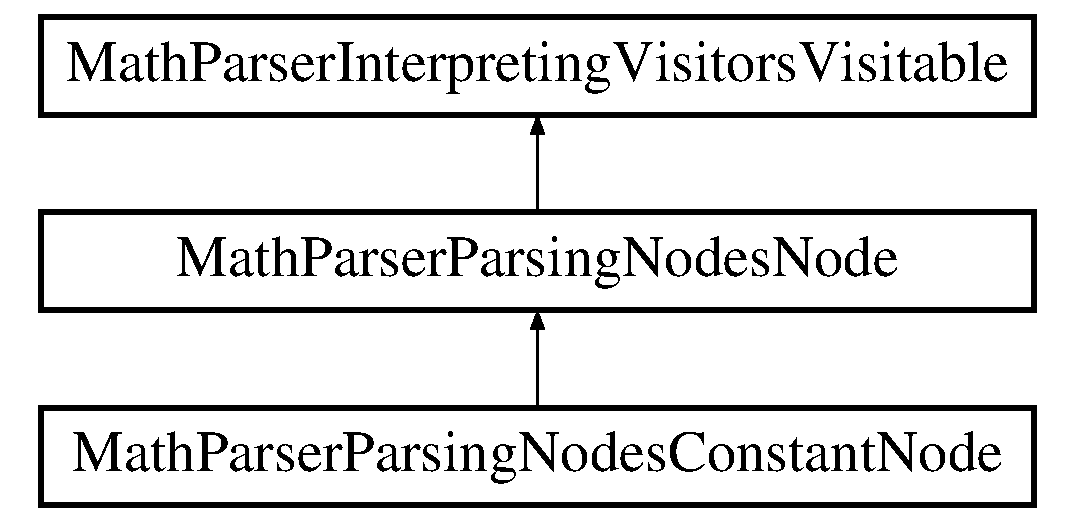
\includegraphics[height=3.000000cm]{classMathParser_1_1Parsing_1_1Nodes_1_1ConstantNode}
\end{center}
\end{figure}
\subsection*{Public Member Functions}
\begin{DoxyCompactItemize}
\item 
\hypertarget{classMathParser_1_1Parsing_1_1Nodes_1_1ConstantNode_a2ad61188ed04bb2fd99dda2db380afbd}{{\bfseries \-\_\-\-\_\-construct} (\$value)}\label{classMathParser_1_1Parsing_1_1Nodes_1_1ConstantNode_a2ad61188ed04bb2fd99dda2db380afbd}

\item 
\hyperlink{classMathParser_1_1Parsing_1_1Nodes_1_1ConstantNode_a537089b5aa92491a904193f449318090}{get\-Name} ()
\item 
\hyperlink{classMathParser_1_1Parsing_1_1Nodes_1_1ConstantNode_a5debc023d33ccf262a4c73569b4af841}{accept} (\hyperlink{interfaceMathParser_1_1Interpreting_1_1Visitors_1_1Visitor}{Visitor} \$visitor)
\begin{DoxyCompactList}\small\item\em Single function in the Visitable interface. \end{DoxyCompactList}\end{DoxyCompactItemize}
\subsection*{Private Attributes}
\begin{DoxyCompactItemize}
\item 
\hypertarget{classMathParser_1_1Parsing_1_1Nodes_1_1ConstantNode_ae9df99dc2bbc8480c637e4f4058f2767}{{\bfseries \$value}}\label{classMathParser_1_1Parsing_1_1Nodes_1_1ConstantNode_ae9df99dc2bbc8480c637e4f4058f2767}

\end{DoxyCompactItemize}
\subsection*{Additional Inherited Members}


\subsection{Member Function Documentation}
\hypertarget{classMathParser_1_1Parsing_1_1Nodes_1_1ConstantNode_a5debc023d33ccf262a4c73569b4af841}{\index{Math\-Parser\-::\-Parsing\-::\-Nodes\-::\-Constant\-Node@{Math\-Parser\-::\-Parsing\-::\-Nodes\-::\-Constant\-Node}!accept@{accept}}
\index{accept@{accept}!MathParser::Parsing::Nodes::ConstantNode@{Math\-Parser\-::\-Parsing\-::\-Nodes\-::\-Constant\-Node}}
\subsubsection[{accept}]{\setlength{\rightskip}{0pt plus 5cm}Math\-Parser\textbackslash{}\-Parsing\textbackslash{}\-Nodes\textbackslash{}\-Constant\-Node\-::accept (
\begin{DoxyParamCaption}
\item[{{\bf Visitor}}]{\$visitor}
\end{DoxyParamCaption}
)}}\label{classMathParser_1_1Parsing_1_1Nodes_1_1ConstantNode_a5debc023d33ccf262a4c73569b4af841}


Single function in the Visitable interface. 

Calling the \hyperlink{classMathParser_1_1Parsing_1_1Nodes_1_1ConstantNode_a5debc023d33ccf262a4c73569b4af841}{accept()} function on a Visitable class, i.\-e. a \hyperlink{classMathParser_1_1Parsing_1_1Nodes_1_1Node}{Node} (or subclass thereof) causes the supplied Visitor to traverse the A\-S\-T.


\begin{DoxyParams}[1]{Parameters}
Visitor & {\em \$visitor} & \\
\hline
\end{DoxyParams}


Implements \hyperlink{interfaceMathParser_1_1Interpreting_1_1Visitors_1_1Visitable_a44418d4bae6a68865102c09dc167409f}{Math\-Parser\textbackslash{}\-Interpreting\textbackslash{}\-Visitors\textbackslash{}\-Visitable}.

\hypertarget{classMathParser_1_1Parsing_1_1Nodes_1_1ConstantNode_a537089b5aa92491a904193f449318090}{\index{Math\-Parser\-::\-Parsing\-::\-Nodes\-::\-Constant\-Node@{Math\-Parser\-::\-Parsing\-::\-Nodes\-::\-Constant\-Node}!get\-Name@{get\-Name}}
\index{get\-Name@{get\-Name}!MathParser::Parsing::Nodes::ConstantNode@{Math\-Parser\-::\-Parsing\-::\-Nodes\-::\-Constant\-Node}}
\subsubsection[{get\-Name}]{\setlength{\rightskip}{0pt plus 5cm}Math\-Parser\textbackslash{}\-Parsing\textbackslash{}\-Nodes\textbackslash{}\-Constant\-Node\-::get\-Name (
\begin{DoxyParamCaption}
{}
\end{DoxyParamCaption}
)}}\label{classMathParser_1_1Parsing_1_1Nodes_1_1ConstantNode_a537089b5aa92491a904193f449318090}

\begin{DoxyRetVals}{Return values}
{\em mixed} & \\
\hline
\end{DoxyRetVals}


The documentation for this class was generated from the following file\-:\begin{DoxyCompactItemize}
\item 
src/\-Math\-Parser/\-Parsing/\-Nodes/Constant\-Node.\-php\end{DoxyCompactItemize}

\hypertarget{classMathParser_1_1Interpreting_1_1Differentiator}{\section{Math\-Parser\textbackslash{}Interpreting\textbackslash{}Differentiator Class Reference}
\label{classMathParser_1_1Interpreting_1_1Differentiator}\index{Math\-Parser\textbackslash{}\-Interpreting\textbackslash{}\-Differentiator@{Math\-Parser\textbackslash{}\-Interpreting\textbackslash{}\-Differentiator}}
}


Differentiate an abstract syntax tree (A\-S\-T).  


Inheritance diagram for Math\-Parser\textbackslash{}Interpreting\textbackslash{}Differentiator\-:\begin{figure}[H]
\begin{center}
\leavevmode
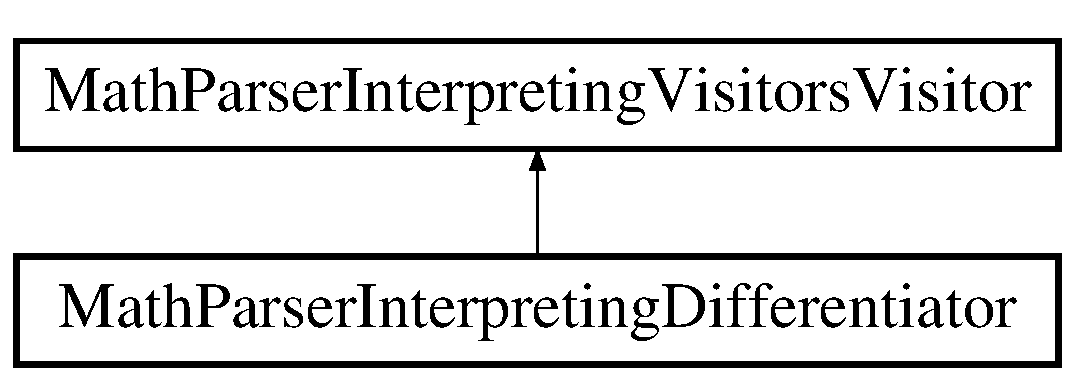
\includegraphics[height=2.000000cm]{classMathParser_1_1Interpreting_1_1Differentiator}
\end{center}
\end{figure}
\subsection*{Public Member Functions}
\begin{DoxyCompactItemize}
\item 
\hyperlink{classMathParser_1_1Interpreting_1_1Differentiator_aa0dd0abee57ec73eeaea9d3341e279f1}{\-\_\-\-\_\-construct} (\$variable)
\begin{DoxyCompactList}\small\item\em Class constructor. \end{DoxyCompactList}\item 
\hyperlink{classMathParser_1_1Interpreting_1_1Differentiator_afed6103538e71009c19d8dd0e37144ee}{visit\-Expression\-Node} (\hyperlink{classMathParser_1_1Parsing_1_1Nodes_1_1ExpressionNode}{Expression\-Node} \$node)
\begin{DoxyCompactList}\small\item\em Differentiate an Expression\-Node. \end{DoxyCompactList}\item 
\hyperlink{classMathParser_1_1Interpreting_1_1Differentiator_aa6fa0932e84b9f3d778387e48c96a9ef}{visit\-Number\-Node} (\hyperlink{classMathParser_1_1Parsing_1_1Nodes_1_1NumberNode}{Number\-Node} \$node)
\begin{DoxyCompactList}\small\item\em Differentiate a Number\-Node. \end{DoxyCompactList}\item 
\hyperlink{classMathParser_1_1Interpreting_1_1Differentiator_a52cc092817e78043da5e6bd86e09ff9f}{visit\-Variable\-Node} (\hyperlink{classMathParser_1_1Parsing_1_1Nodes_1_1VariableNode}{Variable\-Node} \$node)
\begin{DoxyCompactList}\small\item\em Differentiate a Variable\-Node. \end{DoxyCompactList}\item 
\hyperlink{classMathParser_1_1Interpreting_1_1Differentiator_a95027e99c32f63b0689005ff148bee3e}{visit\-Function\-Node} (\hyperlink{classMathParser_1_1Parsing_1_1Nodes_1_1FunctionNode}{Function\-Node} \$node)
\begin{DoxyCompactList}\small\item\em Differentiate a Function\-Node. \end{DoxyCompactList}\item 
\hyperlink{classMathParser_1_1Interpreting_1_1Differentiator_ab89f589a9e372a15997cc08608489e1f}{visit\-Constant\-Node} (\hyperlink{classMathParser_1_1Parsing_1_1Nodes_1_1ConstantNode}{Constant\-Node} \$node)
\begin{DoxyCompactList}\small\item\em Differentiate a Constant\-Node. \end{DoxyCompactList}\end{DoxyCompactItemize}
\subsection*{Private Member Functions}
\begin{DoxyCompactItemize}
\item 
\hyperlink{classMathParser_1_1Interpreting_1_1Differentiator_a0ca77a885d67637f3858e524fe25f94f}{create\-Addition\-Node} (\$x, \$y)
\begin{DoxyCompactList}\small\item\em Create a Node representing 'x+y'. \end{DoxyCompactList}\item 
\hyperlink{classMathParser_1_1Interpreting_1_1Differentiator_aad54652f37938c29c9a426fd568746c8}{create\-Subtraction\-Node} (\$x, \$y)
\begin{DoxyCompactList}\small\item\em Create a Node representing 'x-\/y'. \end{DoxyCompactList}\item 
\hyperlink{classMathParser_1_1Interpreting_1_1Differentiator_a08a7721f2512b45848054ff53ff0a3a5}{create\-Unary\-Minus\-Node} (\$x)
\begin{DoxyCompactList}\small\item\em Create a Node representing '-\/x'. \end{DoxyCompactList}\item 
\hyperlink{classMathParser_1_1Interpreting_1_1Differentiator_a76e94a286700f2913e1f69b985ccd110}{create\-Multiplication\-Node} (\$x, \$y)
\begin{DoxyCompactList}\small\item\em Create a Node representing 'x$\ast$y'. \end{DoxyCompactList}\item 
\hyperlink{classMathParser_1_1Interpreting_1_1Differentiator_a5ba6c413896c0e4d05f579898df23204}{create\-Division\-Node} (\$x, \$y)
\begin{DoxyCompactList}\small\item\em Create a Node representing 'x/y'. \end{DoxyCompactList}\item 
\hyperlink{classMathParser_1_1Interpreting_1_1Differentiator_ac58a93d3f4696e2adbd152f2f78d65c6}{create\-Exponentiation\-Node} (\$x, \$y)
\begin{DoxyCompactList}\small\item\em Create a Node representing 'x$^\wedge$y'. \end{DoxyCompactList}\end{DoxyCompactItemize}
\subsection*{Private Attributes}
\begin{DoxyCompactItemize}
\item 
\hypertarget{classMathParser_1_1Interpreting_1_1Differentiator_af3981989ecf9f68ac5fd5b78ad723910}{\hyperlink{classMathParser_1_1Interpreting_1_1Differentiator_af3981989ecf9f68ac5fd5b78ad723910}{\$variable}}\label{classMathParser_1_1Interpreting_1_1Differentiator_af3981989ecf9f68ac5fd5b78ad723910}

\begin{DoxyCompactList}\small\item\em Variable that we differentiate with respect to. \end{DoxyCompactList}\end{DoxyCompactItemize}


\subsection{Detailed Description}
Differentiate an abstract syntax tree (A\-S\-T). 

Implementation of a Visitor, transforming an A\-S\-T into another A\-S\-T representing the derivative of the original A\-S\-T.

The class implements differentiation rules for all arithmetic operators as well as every elementary function recognized by Std\-Math\-Lexer and Stdmath\-Parser, handling for example the product rule and the chain rule correctly.

To keep the resulting A\-S\-T reasonably simple, a number of simplification rules are built in.

\subsubsection*{Example\-:}


\begin{DoxyCode}
$parser = \textcolor{keyword}{new} StdMathParser();
$f = $parser->parse(\textcolor{stringliteral}{'exp(2x)+xy'});
$ddx = \textcolor{keyword}{new} Differentiator(\textcolor{charliteral}{'x'});     \textcolor{comment}{// Create a d/dx operator}
$df = $f->accept($ddx);             \textcolor{comment}{// $df now contains the AST of '2exp(2x)+y'}
\end{DoxyCode}


T\-O\-D\-O\-: handle user specified functions 

\subsection{Constructor \& Destructor Documentation}
\hypertarget{classMathParser_1_1Interpreting_1_1Differentiator_aa0dd0abee57ec73eeaea9d3341e279f1}{\index{Math\-Parser\-::\-Interpreting\-::\-Differentiator@{Math\-Parser\-::\-Interpreting\-::\-Differentiator}!\-\_\-\-\_\-construct@{\-\_\-\-\_\-construct}}
\index{\-\_\-\-\_\-construct@{\-\_\-\-\_\-construct}!MathParser::Interpreting::Differentiator@{Math\-Parser\-::\-Interpreting\-::\-Differentiator}}
\subsubsection[{\-\_\-\-\_\-construct}]{\setlength{\rightskip}{0pt plus 5cm}Math\-Parser\textbackslash{}\-Interpreting\textbackslash{}\-Differentiator\-::\-\_\-\-\_\-construct (
\begin{DoxyParamCaption}
\item[{}]{\$variable}
\end{DoxyParamCaption}
)}}\label{classMathParser_1_1Interpreting_1_1Differentiator_aa0dd0abee57ec73eeaea9d3341e279f1}


Class constructor. 


\begin{DoxyParams}[1]{Parameters}
string & {\em \$variable} & Differentiation variable \\
\hline
\end{DoxyParams}


\subsection{Member Function Documentation}
\hypertarget{classMathParser_1_1Interpreting_1_1Differentiator_a0ca77a885d67637f3858e524fe25f94f}{\index{Math\-Parser\-::\-Interpreting\-::\-Differentiator@{Math\-Parser\-::\-Interpreting\-::\-Differentiator}!create\-Addition\-Node@{create\-Addition\-Node}}
\index{create\-Addition\-Node@{create\-Addition\-Node}!MathParser::Interpreting::Differentiator@{Math\-Parser\-::\-Interpreting\-::\-Differentiator}}
\subsubsection[{create\-Addition\-Node}]{\setlength{\rightskip}{0pt plus 5cm}Math\-Parser\textbackslash{}\-Interpreting\textbackslash{}\-Differentiator\-::create\-Addition\-Node (
\begin{DoxyParamCaption}
\item[{}]{\$x, }
\item[{}]{\$y}
\end{DoxyParamCaption}
)\hspace{0.3cm}{\ttfamily [private]}}}\label{classMathParser_1_1Interpreting_1_1Differentiator_a0ca77a885d67637f3858e524fe25f94f}


Create a Node representing 'x+y'. 

Using some simplification rules, create a Number\-Node or Expression\-Node giving an A\-S\-T correctly representing 'x+y'.

\paragraph*{Simplification rules\-:}


\begin{DoxyItemize}
\item To simplify the use of the function, convert integer params to Number\-Nodes
\item If \$x and \$y are both Number\-Nodes, return a single Number\-Node containing their sum
\item If \$x or \$y are Number\-Nodes representing 0, return the other term unchanged
\end{DoxyItemize}


\begin{DoxyParams}[1]{Parameters}
Node | int & {\em \$x} & First term \\
\hline
Node | int & {\em \$y} & Second term \\
\hline
\end{DoxyParams}

\begin{DoxyRetVals}{Return values}
{\em Node} & \\
\hline
\end{DoxyRetVals}
\hypertarget{classMathParser_1_1Interpreting_1_1Differentiator_a5ba6c413896c0e4d05f579898df23204}{\index{Math\-Parser\-::\-Interpreting\-::\-Differentiator@{Math\-Parser\-::\-Interpreting\-::\-Differentiator}!create\-Division\-Node@{create\-Division\-Node}}
\index{create\-Division\-Node@{create\-Division\-Node}!MathParser::Interpreting::Differentiator@{Math\-Parser\-::\-Interpreting\-::\-Differentiator}}
\subsubsection[{create\-Division\-Node}]{\setlength{\rightskip}{0pt plus 5cm}Math\-Parser\textbackslash{}\-Interpreting\textbackslash{}\-Differentiator\-::create\-Division\-Node (
\begin{DoxyParamCaption}
\item[{}]{\$x, }
\item[{}]{\$y}
\end{DoxyParamCaption}
)\hspace{0.3cm}{\ttfamily [private]}}}\label{classMathParser_1_1Interpreting_1_1Differentiator_a5ba6c413896c0e4d05f579898df23204}


Create a Node representing 'x/y'. 

Using some simplification rules, create a Number\-Node or Expression\-Node giving an A\-S\-T correctly representing 'x/y'.

\paragraph*{Simplification rules\-:}


\begin{DoxyItemize}
\item To simplify the use of the function, convert integer params to Number\-Nodes
\item If \$x is a Number\-Node representing 0, return 0
\item If \$y is a Number\-Node representing 1, return \$x
\item If \$x and \$y are equal, return '1'
\end{DoxyItemize}


\begin{DoxyParams}[1]{Parameters}
Node | int & {\em \$x} & Numerator \\
\hline
Node | int & {\em \$y} & Denominator \\
\hline
\end{DoxyParams}

\begin{DoxyRetVals}{Return values}
{\em Node} & \\
\hline
\end{DoxyRetVals}
\hypertarget{classMathParser_1_1Interpreting_1_1Differentiator_ac58a93d3f4696e2adbd152f2f78d65c6}{\index{Math\-Parser\-::\-Interpreting\-::\-Differentiator@{Math\-Parser\-::\-Interpreting\-::\-Differentiator}!create\-Exponentiation\-Node@{create\-Exponentiation\-Node}}
\index{create\-Exponentiation\-Node@{create\-Exponentiation\-Node}!MathParser::Interpreting::Differentiator@{Math\-Parser\-::\-Interpreting\-::\-Differentiator}}
\subsubsection[{create\-Exponentiation\-Node}]{\setlength{\rightskip}{0pt plus 5cm}Math\-Parser\textbackslash{}\-Interpreting\textbackslash{}\-Differentiator\-::create\-Exponentiation\-Node (
\begin{DoxyParamCaption}
\item[{}]{\$x, }
\item[{}]{\$y}
\end{DoxyParamCaption}
)\hspace{0.3cm}{\ttfamily [private]}}}\label{classMathParser_1_1Interpreting_1_1Differentiator_ac58a93d3f4696e2adbd152f2f78d65c6}


Create a Node representing 'x$^\wedge$y'. 

Using some simplification rules, create a Number\-Node or Expression\-Node giving an A\-S\-T correctly representing 'x$^\wedge$y'.

\paragraph*{Simplification rules\-:}


\begin{DoxyItemize}
\item To simplify the use of the function, convert integer params to Number\-Nodes
\item If \$x and \$y are both Number\-Nodes, return a single Number\-Node containing x$^\wedge$y
\item If \$y is a Number\-Node representing 0, return '1'
\item If \$y is a Number\-Node representing 1, return \$x
\item If \$x is already a power x=a$^\wedge$b and \$y is a Number\-Node, return a$^\wedge$(b$\ast$y)
\end{DoxyItemize}


\begin{DoxyParams}[1]{Parameters}
Node | int & {\em \$x} & Minuend \\
\hline
Node | int & {\em \$y} & Subtrahend \\
\hline
\end{DoxyParams}

\begin{DoxyRetVals}{Return values}
{\em Node} & \\
\hline
\end{DoxyRetVals}
\hypertarget{classMathParser_1_1Interpreting_1_1Differentiator_a76e94a286700f2913e1f69b985ccd110}{\index{Math\-Parser\-::\-Interpreting\-::\-Differentiator@{Math\-Parser\-::\-Interpreting\-::\-Differentiator}!create\-Multiplication\-Node@{create\-Multiplication\-Node}}
\index{create\-Multiplication\-Node@{create\-Multiplication\-Node}!MathParser::Interpreting::Differentiator@{Math\-Parser\-::\-Interpreting\-::\-Differentiator}}
\subsubsection[{create\-Multiplication\-Node}]{\setlength{\rightskip}{0pt plus 5cm}Math\-Parser\textbackslash{}\-Interpreting\textbackslash{}\-Differentiator\-::create\-Multiplication\-Node (
\begin{DoxyParamCaption}
\item[{}]{\$x, }
\item[{}]{\$y}
\end{DoxyParamCaption}
)\hspace{0.3cm}{\ttfamily [private]}}}\label{classMathParser_1_1Interpreting_1_1Differentiator_a76e94a286700f2913e1f69b985ccd110}


Create a Node representing 'x$\ast$y'. 

Using some simplification rules, create a Number\-Node or Expression\-Node giving an A\-S\-T correctly representing 'x$\ast$y'.

\paragraph*{Simplification rules\-:}


\begin{DoxyItemize}
\item To simplify the use of the function, convert integer params to Number\-Nodes
\item If \$x and \$y are both Number\-Nodes, return a single Number\-Node containing their product
\item If \$x or \$y is a Number\-Node representing 0, return '0'
\item If \$x or \$y is a Number\-Node representing 1, return the other factor
\end{DoxyItemize}


\begin{DoxyParams}[1]{Parameters}
Node | int & {\em \$x} & First factor \\
\hline
Node | int & {\em \$y} & Second factor \\
\hline
\end{DoxyParams}

\begin{DoxyRetVals}{Return values}
{\em Node} & \\
\hline
\end{DoxyRetVals}
\hypertarget{classMathParser_1_1Interpreting_1_1Differentiator_aad54652f37938c29c9a426fd568746c8}{\index{Math\-Parser\-::\-Interpreting\-::\-Differentiator@{Math\-Parser\-::\-Interpreting\-::\-Differentiator}!create\-Subtraction\-Node@{create\-Subtraction\-Node}}
\index{create\-Subtraction\-Node@{create\-Subtraction\-Node}!MathParser::Interpreting::Differentiator@{Math\-Parser\-::\-Interpreting\-::\-Differentiator}}
\subsubsection[{create\-Subtraction\-Node}]{\setlength{\rightskip}{0pt plus 5cm}Math\-Parser\textbackslash{}\-Interpreting\textbackslash{}\-Differentiator\-::create\-Subtraction\-Node (
\begin{DoxyParamCaption}
\item[{}]{\$x, }
\item[{}]{\$y}
\end{DoxyParamCaption}
)\hspace{0.3cm}{\ttfamily [private]}}}\label{classMathParser_1_1Interpreting_1_1Differentiator_aad54652f37938c29c9a426fd568746c8}


Create a Node representing 'x-\/y'. 

Using some simplification rules, create a Number\-Node or Expression\-Node giving an A\-S\-T correctly representing 'x-\/y'.

\paragraph*{Simplification rules\-:}


\begin{DoxyItemize}
\item To simplify the use of the function, convert integer params to Number\-Nodes
\item If \$y is null, return a unary minus node '-\/x' instead
\item If \$x and \$y are both Number\-Nodes, return a single Number\-Node containing their difference
\item If \$y is a Number\-Node representing 0, return \$x unchanged
\item If \$x and \$y are equal, return '0'
\end{DoxyItemize}


\begin{DoxyParams}[1]{Parameters}
Node | int & {\em \$x} & Minuend \\
\hline
Node | int & {\em \$y} & Subtrahend \\
\hline
\end{DoxyParams}

\begin{DoxyRetVals}{Return values}
{\em Node} & \\
\hline
\end{DoxyRetVals}
\hypertarget{classMathParser_1_1Interpreting_1_1Differentiator_a08a7721f2512b45848054ff53ff0a3a5}{\index{Math\-Parser\-::\-Interpreting\-::\-Differentiator@{Math\-Parser\-::\-Interpreting\-::\-Differentiator}!create\-Unary\-Minus\-Node@{create\-Unary\-Minus\-Node}}
\index{create\-Unary\-Minus\-Node@{create\-Unary\-Minus\-Node}!MathParser::Interpreting::Differentiator@{Math\-Parser\-::\-Interpreting\-::\-Differentiator}}
\subsubsection[{create\-Unary\-Minus\-Node}]{\setlength{\rightskip}{0pt plus 5cm}Math\-Parser\textbackslash{}\-Interpreting\textbackslash{}\-Differentiator\-::create\-Unary\-Minus\-Node (
\begin{DoxyParamCaption}
\item[{}]{\$x}
\end{DoxyParamCaption}
)\hspace{0.3cm}{\ttfamily [private]}}}\label{classMathParser_1_1Interpreting_1_1Differentiator_a08a7721f2512b45848054ff53ff0a3a5}


Create a Node representing '-\/x'. 

Using some simplification rules, create a Number\-Node or Expression\-Node giving an A\-S\-T correctly representing '-\/x'.

\paragraph*{Simplification rules\-:}


\begin{DoxyItemize}
\item To simplify the use of the function, convert integer params to Number\-Nodes
\item If \$x is a Number\-Nodes, return a single Number\-Node containing its negative
\item If \$x already is a unary minus, 'x=-\/y', return y
\end{DoxyItemize}


\begin{DoxyParams}[1]{Parameters}
Node | int & {\em \$x} & Operand \\
\hline
\end{DoxyParams}

\begin{DoxyRetVals}{Return values}
{\em Node} & \\
\hline
\end{DoxyRetVals}
\hypertarget{classMathParser_1_1Interpreting_1_1Differentiator_ab89f589a9e372a15997cc08608489e1f}{\index{Math\-Parser\-::\-Interpreting\-::\-Differentiator@{Math\-Parser\-::\-Interpreting\-::\-Differentiator}!visit\-Constant\-Node@{visit\-Constant\-Node}}
\index{visit\-Constant\-Node@{visit\-Constant\-Node}!MathParser::Interpreting::Differentiator@{Math\-Parser\-::\-Interpreting\-::\-Differentiator}}
\subsubsection[{visit\-Constant\-Node}]{\setlength{\rightskip}{0pt plus 5cm}Math\-Parser\textbackslash{}\-Interpreting\textbackslash{}\-Differentiator\-::visit\-Constant\-Node (
\begin{DoxyParamCaption}
\item[{{\bf Constant\-Node}}]{\$node}
\end{DoxyParamCaption}
)}}\label{classMathParser_1_1Interpreting_1_1Differentiator_ab89f589a9e372a15997cc08608489e1f}


Differentiate a Constant\-Node. 

Create a Number\-Node representing '0'. (The derivative of a constant is indentically 0).


\begin{DoxyParams}[1]{Parameters}
Constant\-Node & {\em \$node} & A\-S\-T to be differentiated \\
\hline
\end{DoxyParams}

\begin{DoxyRetVals}{Return values}
{\em Node} & \\
\hline
\end{DoxyRetVals}


Implements \hyperlink{interfaceMathParser_1_1Interpreting_1_1Visitors_1_1Visitor_ac694089225b20c9f848bcfb0a5e600f0}{Math\-Parser\textbackslash{}\-Interpreting\textbackslash{}\-Visitors\textbackslash{}\-Visitor}.

\hypertarget{classMathParser_1_1Interpreting_1_1Differentiator_afed6103538e71009c19d8dd0e37144ee}{\index{Math\-Parser\-::\-Interpreting\-::\-Differentiator@{Math\-Parser\-::\-Interpreting\-::\-Differentiator}!visit\-Expression\-Node@{visit\-Expression\-Node}}
\index{visit\-Expression\-Node@{visit\-Expression\-Node}!MathParser::Interpreting::Differentiator@{Math\-Parser\-::\-Interpreting\-::\-Differentiator}}
\subsubsection[{visit\-Expression\-Node}]{\setlength{\rightskip}{0pt plus 5cm}Math\-Parser\textbackslash{}\-Interpreting\textbackslash{}\-Differentiator\-::visit\-Expression\-Node (
\begin{DoxyParamCaption}
\item[{{\bf Expression\-Node}}]{\$node}
\end{DoxyParamCaption}
)}}\label{classMathParser_1_1Interpreting_1_1Differentiator_afed6103538e71009c19d8dd0e37144ee}


Differentiate an Expression\-Node. 

Using the usual rules for differentiating, create an Expression\-Node giving an A\-S\-T correctly representing the derivative {\ttfamily (x op y)'} where {\ttfamily op} is one of {\ttfamily +}, {\ttfamily -\/}, {\ttfamily $\ast$}, {\ttfamily /} or {\ttfamily $^\wedge$}

\paragraph*{Differentiation rules\-:}


\begin{DoxyItemize}
\item \textbackslash{}( (f+g)' = f' + g' \textbackslash{})
\item \textbackslash{}( (f-\/g) ' = f' -\/ g' \textbackslash{})
\item \textbackslash{}( (-\/f)' = -\/f' \textbackslash{})
\item \textbackslash{}( (f$\ast$g)' = f'g + f g' \textbackslash{})
\item \textbackslash{}( (f/g)' = (f' g -\/ f g')/g$^\wedge$2 \textbackslash{})
\item \textbackslash{}( (f$^\wedge$g)' = f$^\wedge$g (g' \textbackslash{}log(f) + g/f) \textbackslash{}) with a simpler expression when g is a Number\-Node
\end{DoxyItemize}


\begin{DoxyExceptions}{Exceptions}
{\em Unknown\-Operator\-Exception} & if the operator is something other than {\ttfamily +}, {\ttfamily -\/}, {\ttfamily $\ast$}, {\ttfamily /} or {\ttfamily $^\wedge$}\\
\hline
\end{DoxyExceptions}

\begin{DoxyParams}[1]{Parameters}
Expression\-Node & {\em \$node} & A\-S\-T to be differentiated \\
\hline
\end{DoxyParams}

\begin{DoxyRetVals}{Return values}
{\em Node} & \\
\hline
\end{DoxyRetVals}


Implements \hyperlink{interfaceMathParser_1_1Interpreting_1_1Visitors_1_1Visitor_a201489f6ae0ccc3c25ff153a57994fa1}{Math\-Parser\textbackslash{}\-Interpreting\textbackslash{}\-Visitors\textbackslash{}\-Visitor}.

\hypertarget{classMathParser_1_1Interpreting_1_1Differentiator_a95027e99c32f63b0689005ff148bee3e}{\index{Math\-Parser\-::\-Interpreting\-::\-Differentiator@{Math\-Parser\-::\-Interpreting\-::\-Differentiator}!visit\-Function\-Node@{visit\-Function\-Node}}
\index{visit\-Function\-Node@{visit\-Function\-Node}!MathParser::Interpreting::Differentiator@{Math\-Parser\-::\-Interpreting\-::\-Differentiator}}
\subsubsection[{visit\-Function\-Node}]{\setlength{\rightskip}{0pt plus 5cm}Math\-Parser\textbackslash{}\-Interpreting\textbackslash{}\-Differentiator\-::visit\-Function\-Node (
\begin{DoxyParamCaption}
\item[{{\bf Function\-Node}}]{\$node}
\end{DoxyParamCaption}
)}}\label{classMathParser_1_1Interpreting_1_1Differentiator_a95027e99c32f63b0689005ff148bee3e}


Differentiate a Function\-Node. 

Create an Expression\-Node giving an A\-S\-T correctly representing the derivative {\ttfamily f'} where {\ttfamily f} is an elementary function.

\paragraph*{Differentiation rules\-:}


\begin{DoxyItemize}
\item \textbackslash{}( \textbackslash{}sin(f(x))' = f'(x) \textbackslash{}cos(f(x)) \textbackslash{})
\item \textbackslash{}( \textbackslash{}cos(f(x))' = -\/f'(x) \textbackslash{}sin(f(x)) \textbackslash{})
\item \textbackslash{}( \textbackslash{}tan(f(x))' = f'(x) (1 + \textbackslash{}tan(f(x))$^\wedge$2 \textbackslash{})
\item \textbackslash{}( \textbackslash{}operatorname\{cot\}(f(x))' = f'(x) (-\/1 + \textbackslash{}operatorname\{cot\}(f(x))$^\wedge$2 \textbackslash{})
\item \textbackslash{}( \textbackslash{}arcsin(f(x))' = f'(x) / \textbackslash{}sqrt\{1-\/f(x)$^\wedge$2\} \textbackslash{})
\item \textbackslash{}( \textbackslash{}arccos(f(x))' = -\/f'(x) / \textbackslash{}sqrt\{1-\/f(x)$^\wedge$2\} \textbackslash{})
\item \textbackslash{}( \textbackslash{}arctan(f(x))' = f'(x) / (1+f(x)$^\wedge$2) \textbackslash{})
\item \textbackslash{}( \textbackslash{}operatorname\{arccot\}(f(x))' = -\/f'(x) / (1+f(x)$^\wedge$2) \textbackslash{})
\item \textbackslash{}( \textbackslash{}exp(f(x))' = f'(x) \textbackslash{}exp(f(x)) \textbackslash{})
\item \textbackslash{}( \textbackslash{}log(f(x))' = f'(x) / f(x) \textbackslash{})
\item \textbackslash{}( \textbackslash{}ln(f(x))' = f'(x) / (\textbackslash{}log(10) $\ast$ f(x)) \textbackslash{})
\item \textbackslash{}( \textbackslash{}sqrt\{f(x)\}' = f'(x) / (2 \textbackslash{}sqrt\{f(x)\} \textbackslash{})
\item \textbackslash{}( \textbackslash{}sinh(f(x))' = f'(x) \textbackslash{}cosh(f(x)) \textbackslash{})
\item \textbackslash{}( \textbackslash{}cosh(f(x))' = f'(x) \textbackslash{}sinh(f(x)) \textbackslash{})
\item \textbackslash{}( \textbackslash{}tanh(f(x))' = f'(x) (1-\/\textbackslash{}tanh(f(x))$^\wedge$2) \textbackslash{})
\item \textbackslash{}( \textbackslash{}operatorname\{coth\}(f(x))' = f'(x) (1-\/\textbackslash{}operatorname\{coth\}(f(x))$^\wedge$2) \textbackslash{})
\item \textbackslash{}( \textbackslash{}operatorname\{arsinh\}(f(x))' = f'(x) / \textbackslash{}sqrt\{f(x)$^\wedge$2+1\} \textbackslash{})
\item \textbackslash{}( \textbackslash{}operatorname\{arcosh\}(f(x))' = f'(x) / \textbackslash{}sqrt\{f(x)$^\wedge$2-\/1\} \textbackslash{})
\item \textbackslash{}( \textbackslash{}operatorname\{artanh\}(f(x))' = f'(x) (1-\/f(x)$^\wedge$2) \textbackslash{})
\item \textbackslash{}( \textbackslash{}operatorname\{arcoth\}(f(x))' = f'(x) (1-\/f(x)$^\wedge$2) \textbackslash{})
\end{DoxyItemize}


\begin{DoxyExceptions}{Exceptions}
{\em Unknown\-Function\-Exception} & if the function name doesn't match one of the above\\
\hline
\end{DoxyExceptions}

\begin{DoxyParams}[1]{Parameters}
Function\-Node & {\em \$node} & A\-S\-T to be differentiated \\
\hline
\end{DoxyParams}

\begin{DoxyRetVals}{Return values}
{\em Node} & \\
\hline
\end{DoxyRetVals}


Implements \hyperlink{interfaceMathParser_1_1Interpreting_1_1Visitors_1_1Visitor_a497e4a990f99689616c25e76b0ec6ef1}{Math\-Parser\textbackslash{}\-Interpreting\textbackslash{}\-Visitors\textbackslash{}\-Visitor}.

\hypertarget{classMathParser_1_1Interpreting_1_1Differentiator_aa6fa0932e84b9f3d778387e48c96a9ef}{\index{Math\-Parser\-::\-Interpreting\-::\-Differentiator@{Math\-Parser\-::\-Interpreting\-::\-Differentiator}!visit\-Number\-Node@{visit\-Number\-Node}}
\index{visit\-Number\-Node@{visit\-Number\-Node}!MathParser::Interpreting::Differentiator@{Math\-Parser\-::\-Interpreting\-::\-Differentiator}}
\subsubsection[{visit\-Number\-Node}]{\setlength{\rightskip}{0pt plus 5cm}Math\-Parser\textbackslash{}\-Interpreting\textbackslash{}\-Differentiator\-::visit\-Number\-Node (
\begin{DoxyParamCaption}
\item[{{\bf Number\-Node}}]{\$node}
\end{DoxyParamCaption}
)}}\label{classMathParser_1_1Interpreting_1_1Differentiator_aa6fa0932e84b9f3d778387e48c96a9ef}


Differentiate a Number\-Node. 

Create a Number\-Node representing '0'. (The derivative of a constant is indentically 0).


\begin{DoxyParams}[1]{Parameters}
Number\-Node & {\em \$node} & A\-S\-T to be differentiated \\
\hline
\end{DoxyParams}

\begin{DoxyRetVals}{Return values}
{\em Node} & \\
\hline
\end{DoxyRetVals}


Implements \hyperlink{interfaceMathParser_1_1Interpreting_1_1Visitors_1_1Visitor_acbcd1cbecf76ba51c893a49746162dc1}{Math\-Parser\textbackslash{}\-Interpreting\textbackslash{}\-Visitors\textbackslash{}\-Visitor}.

\hypertarget{classMathParser_1_1Interpreting_1_1Differentiator_a52cc092817e78043da5e6bd86e09ff9f}{\index{Math\-Parser\-::\-Interpreting\-::\-Differentiator@{Math\-Parser\-::\-Interpreting\-::\-Differentiator}!visit\-Variable\-Node@{visit\-Variable\-Node}}
\index{visit\-Variable\-Node@{visit\-Variable\-Node}!MathParser::Interpreting::Differentiator@{Math\-Parser\-::\-Interpreting\-::\-Differentiator}}
\subsubsection[{visit\-Variable\-Node}]{\setlength{\rightskip}{0pt plus 5cm}Math\-Parser\textbackslash{}\-Interpreting\textbackslash{}\-Differentiator\-::visit\-Variable\-Node (
\begin{DoxyParamCaption}
\item[{{\bf Variable\-Node}}]{\$node}
\end{DoxyParamCaption}
)}}\label{classMathParser_1_1Interpreting_1_1Differentiator_a52cc092817e78043da5e6bd86e09ff9f}


Differentiate a Variable\-Node. 

Create a Number\-Node representing '0' or '1' depending on the differetiation variable.


\begin{DoxyParams}[1]{Parameters}
Number\-Node & {\em \$node} & A\-S\-T to be differentiated \\
\hline
\end{DoxyParams}

\begin{DoxyRetVals}{Return values}
{\em Node} & \\
\hline
\end{DoxyRetVals}


Implements \hyperlink{interfaceMathParser_1_1Interpreting_1_1Visitors_1_1Visitor_a292630a7204dadd96877d8182f38deb0}{Math\-Parser\textbackslash{}\-Interpreting\textbackslash{}\-Visitors\textbackslash{}\-Visitor}.



The documentation for this class was generated from the following file\-:\begin{DoxyCompactItemize}
\item 
src/\-Math\-Parser/\-Interpreting/Differentiator.\-php\end{DoxyCompactItemize}

\hypertarget{classMathParser_1_1Exceptions_1_1DivisionByZeroException}{\section{Math\-Parser\textbackslash{}Exceptions\textbackslash{}Division\-By\-Zero\-Exception Class Reference}
\label{classMathParser_1_1Exceptions_1_1DivisionByZeroException}\index{Math\-Parser\textbackslash{}\-Exceptions\textbackslash{}\-Division\-By\-Zero\-Exception@{Math\-Parser\textbackslash{}\-Exceptions\textbackslash{}\-Division\-By\-Zero\-Exception}}
}
Inheritance diagram for Math\-Parser\textbackslash{}Exceptions\textbackslash{}Division\-By\-Zero\-Exception\-:\begin{figure}[H]
\begin{center}
\leavevmode
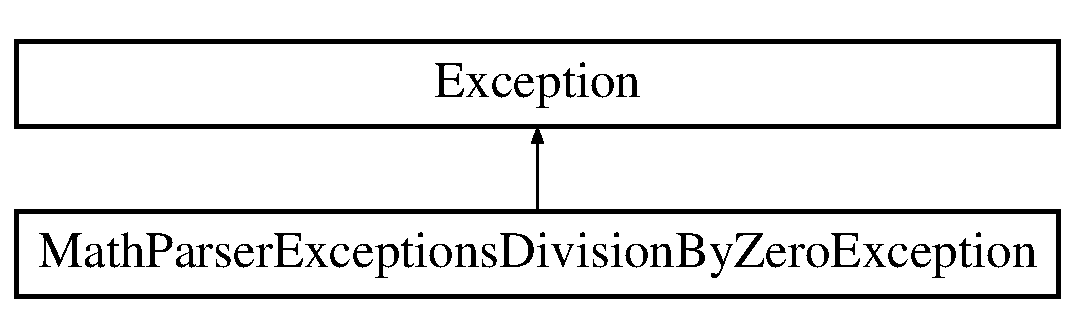
\includegraphics[height=2.000000cm]{classMathParser_1_1Exceptions_1_1DivisionByZeroException}
\end{center}
\end{figure}


The documentation for this class was generated from the following file\-:\begin{DoxyCompactItemize}
\item 
src/\-Math\-Parser/\-Exceptions/Division\-By\-Zero\-Exception.\-php\end{DoxyCompactItemize}

\hypertarget{classMathParser_1_1Interpreting_1_1Evaluator}{\section{Math\-Parser\textbackslash{}Interpreting\textbackslash{}Evaluator Class Reference}
\label{classMathParser_1_1Interpreting_1_1Evaluator}\index{Math\-Parser\textbackslash{}\-Interpreting\textbackslash{}\-Evaluator@{Math\-Parser\textbackslash{}\-Interpreting\textbackslash{}\-Evaluator}}
}


Evalutate a parsed mathematical expression.  


Inheritance diagram for Math\-Parser\textbackslash{}Interpreting\textbackslash{}Evaluator\-:\begin{figure}[H]
\begin{center}
\leavevmode
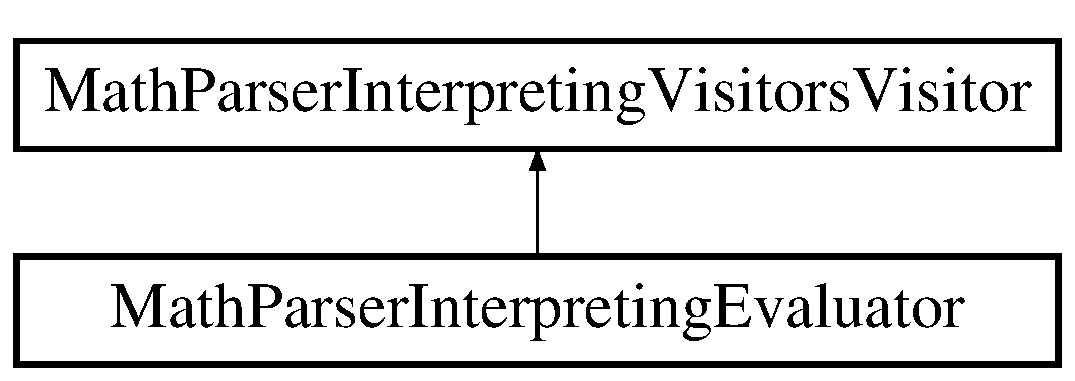
\includegraphics[height=2.000000cm]{classMathParser_1_1Interpreting_1_1Evaluator}
\end{center}
\end{figure}
\subsection*{Public Member Functions}
\begin{DoxyCompactItemize}
\item 
\hypertarget{classMathParser_1_1Interpreting_1_1Evaluator_aa41d08bd9b0d8b204c3ad8d04ce0ca9e}{{\bfseries \-\_\-\-\_\-construct} (\$variables=null)}\label{classMathParser_1_1Interpreting_1_1Evaluator_aa41d08bd9b0d8b204c3ad8d04ce0ca9e}

\item 
\hyperlink{classMathParser_1_1Interpreting_1_1Evaluator_ada67630eccaad9b2c496eaf320b9303c}{set\-Variables} (\$variables)
\begin{DoxyCompactList}\small\item\em Update the variables used for evaluating. \end{DoxyCompactList}\item 
\hyperlink{classMathParser_1_1Interpreting_1_1Evaluator_af8dbfe9e89ba2450ca2e070dc39e47e8}{visit\-Expression\-Node} (\hyperlink{classMathParser_1_1Parsing_1_1Nodes_1_1ExpressionNode}{Expression\-Node} \$node)
\begin{DoxyCompactList}\small\item\em Evaluate an Expression\-Node. \end{DoxyCompactList}\item 
\hyperlink{classMathParser_1_1Interpreting_1_1Evaluator_a1ce6d1017e55901a580256a2f1edd027}{visit\-Number\-Node} (\hyperlink{classMathParser_1_1Parsing_1_1Nodes_1_1NumberNode}{Number\-Node} \$node)
\begin{DoxyCompactList}\small\item\em Evaluate a Number\-Node. \end{DoxyCompactList}\item 
\hyperlink{classMathParser_1_1Interpreting_1_1Evaluator_a67cd18f0dc33f6e2755008053cd8cc0a}{visit\-Variable\-Node} (\hyperlink{classMathParser_1_1Parsing_1_1Nodes_1_1VariableNode}{Variable\-Node} \$node)
\begin{DoxyCompactList}\small\item\em Evaluate a Variable\-Node. \end{DoxyCompactList}\item 
\hyperlink{classMathParser_1_1Interpreting_1_1Evaluator_a455ab6d3c963aeb2e3ad0c731c8bc081}{visit\-Function\-Node} (\hyperlink{classMathParser_1_1Parsing_1_1Nodes_1_1FunctionNode}{Function\-Node} \$node)
\begin{DoxyCompactList}\small\item\em Evaluate a Function\-Node. \end{DoxyCompactList}\item 
\hyperlink{classMathParser_1_1Interpreting_1_1Evaluator_a257b2634d88050c7e51de91c5f09b7b8}{visit\-Constant\-Node} (\hyperlink{classMathParser_1_1Parsing_1_1Nodes_1_1ConstantNode}{Constant\-Node} \$node)
\begin{DoxyCompactList}\small\item\em Evaluate a Constant\-Node. \end{DoxyCompactList}\end{DoxyCompactItemize}
\subsection*{Private Attributes}
\begin{DoxyCompactItemize}
\item 
\hypertarget{classMathParser_1_1Interpreting_1_1Evaluator_ac43d7a3d54117fba595e227fef653e5d}{{\bfseries \$variables}}\label{classMathParser_1_1Interpreting_1_1Evaluator_ac43d7a3d54117fba595e227fef653e5d}

\end{DoxyCompactItemize}


\subsection{Detailed Description}
Evalutate a parsed mathematical expression. 

Implementation of a Visitor, transforming an A\-S\-T into a floating point number, giving the {\itshape value} of the expression represented by the A\-S\-T.

The class implements evaluation of all all arithmetic operators as well as every elementary function and predefined constant recognized by Std\-Math\-Lexer and Stdmath\-Parser.

\subsubsection*{Example\-:}


\begin{DoxyCode}
$parser = \textcolor{keyword}{new} StdMathParser();
$f = $parser->parse(\textcolor{stringliteral}{'exp(2x)+xy'});
$evaluator = \textcolor{keyword}{new} Evaluator();
$evaluator->setVariables([ \textcolor{charliteral}{'x'} => 1, \textcolor{charliteral}{'y'} => \textcolor{stringliteral}{'-1'} ]);
result = $f->accept($evaluator);    \textcolor{comment}{// Evaluate $f using x=1, y=-1}
\end{DoxyCode}


T\-O\-D\-O\-: handle user specified functions 

\subsection{Member Function Documentation}
\hypertarget{classMathParser_1_1Interpreting_1_1Evaluator_ada67630eccaad9b2c496eaf320b9303c}{\index{Math\-Parser\-::\-Interpreting\-::\-Evaluator@{Math\-Parser\-::\-Interpreting\-::\-Evaluator}!set\-Variables@{set\-Variables}}
\index{set\-Variables@{set\-Variables}!MathParser::Interpreting::Evaluator@{Math\-Parser\-::\-Interpreting\-::\-Evaluator}}
\subsubsection[{set\-Variables}]{\setlength{\rightskip}{0pt plus 5cm}Math\-Parser\textbackslash{}\-Interpreting\textbackslash{}\-Evaluator\-::set\-Variables (
\begin{DoxyParamCaption}
\item[{}]{\$variables}
\end{DoxyParamCaption}
)}}\label{classMathParser_1_1Interpreting_1_1Evaluator_ada67630eccaad9b2c496eaf320b9303c}


Update the variables used for evaluating. 


\begin{DoxyParams}[1]{Parameters}
array & {\em \$variables} & Key/value pair holding current variable values \\
\hline
\end{DoxyParams}

\begin{DoxyRetVals}{Return values}
{\em void} & \\
\hline
\end{DoxyRetVals}
\hypertarget{classMathParser_1_1Interpreting_1_1Evaluator_a257b2634d88050c7e51de91c5f09b7b8}{\index{Math\-Parser\-::\-Interpreting\-::\-Evaluator@{Math\-Parser\-::\-Interpreting\-::\-Evaluator}!visit\-Constant\-Node@{visit\-Constant\-Node}}
\index{visit\-Constant\-Node@{visit\-Constant\-Node}!MathParser::Interpreting::Evaluator@{Math\-Parser\-::\-Interpreting\-::\-Evaluator}}
\subsubsection[{visit\-Constant\-Node}]{\setlength{\rightskip}{0pt plus 5cm}Math\-Parser\textbackslash{}\-Interpreting\textbackslash{}\-Evaluator\-::visit\-Constant\-Node (
\begin{DoxyParamCaption}
\item[{{\bf Constant\-Node}}]{\$node}
\end{DoxyParamCaption}
)}}\label{classMathParser_1_1Interpreting_1_1Evaluator_a257b2634d88050c7e51de91c5f09b7b8}


Evaluate a Constant\-Node. 

Returns the value of a Constant\-Node recognized by Std\-Math\-Lexer and \hyperlink{classMathParser_1_1StdMathParser}{Std\-Math\-Parser}.

\begin{DoxySeeAlso}{See Also}
Math\-Parser\-::\-Lexer\-::\-Std\-Math\-Lexer Std\-Math\-Lexer 

\hyperlink{classMathParser_1_1StdMathParser}{Math\-Parser\-::\-Std\-Math\-Parser} \hyperlink{classMathParser_1_1StdMathParser}{Std\-Math\-Parser} 
\end{DoxySeeAlso}

\begin{DoxyExceptions}{Exceptions}
{\em Unknown\-Constant\-Exception} & if the variable respresented by the Constant\-Node is {\itshape not} recognized.\\
\hline
\end{DoxyExceptions}

\begin{DoxyParams}[1]{Parameters}
Constant\-Node & {\em \$node} & A\-S\-T to be evaluated \\
\hline
\end{DoxyParams}

\begin{DoxyRetVals}{Return values}
{\em float} & \\
\hline
\end{DoxyRetVals}


Implements \hyperlink{interfaceMathParser_1_1Interpreting_1_1Visitors_1_1Visitor_ac694089225b20c9f848bcfb0a5e600f0}{Math\-Parser\textbackslash{}\-Interpreting\textbackslash{}\-Visitors\textbackslash{}\-Visitor}.

\hypertarget{classMathParser_1_1Interpreting_1_1Evaluator_af8dbfe9e89ba2450ca2e070dc39e47e8}{\index{Math\-Parser\-::\-Interpreting\-::\-Evaluator@{Math\-Parser\-::\-Interpreting\-::\-Evaluator}!visit\-Expression\-Node@{visit\-Expression\-Node}}
\index{visit\-Expression\-Node@{visit\-Expression\-Node}!MathParser::Interpreting::Evaluator@{Math\-Parser\-::\-Interpreting\-::\-Evaluator}}
\subsubsection[{visit\-Expression\-Node}]{\setlength{\rightskip}{0pt plus 5cm}Math\-Parser\textbackslash{}\-Interpreting\textbackslash{}\-Evaluator\-::visit\-Expression\-Node (
\begin{DoxyParamCaption}
\item[{{\bf Expression\-Node}}]{\$node}
\end{DoxyParamCaption}
)}}\label{classMathParser_1_1Interpreting_1_1Evaluator_af8dbfe9e89ba2450ca2e070dc39e47e8}


Evaluate an Expression\-Node. 

Computes the value of an Expression\-Node {\ttfamily x op y} where {\ttfamily op} is one of {\ttfamily +}, {\ttfamily -\/}, {\ttfamily $\ast$}, {\ttfamily /} or {\ttfamily $^\wedge$}


\begin{DoxyExceptions}{Exceptions}
{\em Unknown\-Operator\-Exception} & if the operator is something other than {\ttfamily +}, {\ttfamily -\/}, {\ttfamily $\ast$}, {\ttfamily /} or {\ttfamily $^\wedge$}\\
\hline
\end{DoxyExceptions}

\begin{DoxyParams}[1]{Parameters}
Expression\-Node & {\em \$node} & A\-S\-T to be evaluated \\
\hline
\end{DoxyParams}

\begin{DoxyRetVals}{Return values}
{\em float} & \\
\hline
\end{DoxyRetVals}


Implements \hyperlink{interfaceMathParser_1_1Interpreting_1_1Visitors_1_1Visitor_a201489f6ae0ccc3c25ff153a57994fa1}{Math\-Parser\textbackslash{}\-Interpreting\textbackslash{}\-Visitors\textbackslash{}\-Visitor}.

\hypertarget{classMathParser_1_1Interpreting_1_1Evaluator_a455ab6d3c963aeb2e3ad0c731c8bc081}{\index{Math\-Parser\-::\-Interpreting\-::\-Evaluator@{Math\-Parser\-::\-Interpreting\-::\-Evaluator}!visit\-Function\-Node@{visit\-Function\-Node}}
\index{visit\-Function\-Node@{visit\-Function\-Node}!MathParser::Interpreting::Evaluator@{Math\-Parser\-::\-Interpreting\-::\-Evaluator}}
\subsubsection[{visit\-Function\-Node}]{\setlength{\rightskip}{0pt plus 5cm}Math\-Parser\textbackslash{}\-Interpreting\textbackslash{}\-Evaluator\-::visit\-Function\-Node (
\begin{DoxyParamCaption}
\item[{{\bf Function\-Node}}]{\$node}
\end{DoxyParamCaption}
)}}\label{classMathParser_1_1Interpreting_1_1Evaluator_a455ab6d3c963aeb2e3ad0c731c8bc081}


Evaluate a Function\-Node. 

Computes the value of a Function\-Node {\ttfamily f(x)}, where f is an elementary function recognized by Std\-Math\-Lexer and \hyperlink{classMathParser_1_1StdMathParser}{Std\-Math\-Parser}.

\begin{DoxySeeAlso}{See Also}
Math\-Parser\-::\-Lexer\-::\-Std\-Math\-Lexer Std\-Math\-Lexer 

\hyperlink{classMathParser_1_1StdMathParser}{Math\-Parser\-::\-Std\-Math\-Parser} \hyperlink{classMathParser_1_1StdMathParser}{Std\-Math\-Parser} 
\end{DoxySeeAlso}

\begin{DoxyExceptions}{Exceptions}
{\em Unknown\-Function\-Exception} & if the function respresented by the Function\-Node is {\itshape not} recognized.\\
\hline
\end{DoxyExceptions}

\begin{DoxyParams}[1]{Parameters}
Function\-Node & {\em \$node} & A\-S\-T to be evaluated \\
\hline
\end{DoxyParams}

\begin{DoxyRetVals}{Return values}
{\em float} & \\
\hline
\end{DoxyRetVals}


Implements \hyperlink{interfaceMathParser_1_1Interpreting_1_1Visitors_1_1Visitor_a497e4a990f99689616c25e76b0ec6ef1}{Math\-Parser\textbackslash{}\-Interpreting\textbackslash{}\-Visitors\textbackslash{}\-Visitor}.

\hypertarget{classMathParser_1_1Interpreting_1_1Evaluator_a1ce6d1017e55901a580256a2f1edd027}{\index{Math\-Parser\-::\-Interpreting\-::\-Evaluator@{Math\-Parser\-::\-Interpreting\-::\-Evaluator}!visit\-Number\-Node@{visit\-Number\-Node}}
\index{visit\-Number\-Node@{visit\-Number\-Node}!MathParser::Interpreting::Evaluator@{Math\-Parser\-::\-Interpreting\-::\-Evaluator}}
\subsubsection[{visit\-Number\-Node}]{\setlength{\rightskip}{0pt plus 5cm}Math\-Parser\textbackslash{}\-Interpreting\textbackslash{}\-Evaluator\-::visit\-Number\-Node (
\begin{DoxyParamCaption}
\item[{{\bf Number\-Node}}]{\$node}
\end{DoxyParamCaption}
)}}\label{classMathParser_1_1Interpreting_1_1Evaluator_a1ce6d1017e55901a580256a2f1edd027}


Evaluate a Number\-Node. 

Retuns the value of an Number\-Node


\begin{DoxyParams}[1]{Parameters}
Number\-Node & {\em \$node} & A\-S\-T to be evaluated \\
\hline
\end{DoxyParams}

\begin{DoxyRetVals}{Return values}
{\em float} & \\
\hline
\end{DoxyRetVals}


Implements \hyperlink{interfaceMathParser_1_1Interpreting_1_1Visitors_1_1Visitor_acbcd1cbecf76ba51c893a49746162dc1}{Math\-Parser\textbackslash{}\-Interpreting\textbackslash{}\-Visitors\textbackslash{}\-Visitor}.

\hypertarget{classMathParser_1_1Interpreting_1_1Evaluator_a67cd18f0dc33f6e2755008053cd8cc0a}{\index{Math\-Parser\-::\-Interpreting\-::\-Evaluator@{Math\-Parser\-::\-Interpreting\-::\-Evaluator}!visit\-Variable\-Node@{visit\-Variable\-Node}}
\index{visit\-Variable\-Node@{visit\-Variable\-Node}!MathParser::Interpreting::Evaluator@{Math\-Parser\-::\-Interpreting\-::\-Evaluator}}
\subsubsection[{visit\-Variable\-Node}]{\setlength{\rightskip}{0pt plus 5cm}Math\-Parser\textbackslash{}\-Interpreting\textbackslash{}\-Evaluator\-::visit\-Variable\-Node (
\begin{DoxyParamCaption}
\item[{{\bf Variable\-Node}}]{\$node}
\end{DoxyParamCaption}
)}}\label{classMathParser_1_1Interpreting_1_1Evaluator_a67cd18f0dc33f6e2755008053cd8cc0a}


Evaluate a Variable\-Node. 

Returns the current value of a Variable\-Node, as defined either by the constructor or set using the {\ttfamily \hyperlink{classMathParser_1_1Interpreting_1_1Evaluator_ada67630eccaad9b2c496eaf320b9303c}{Evaluator\-::set\-Variables()}} method.

\begin{DoxySeeAlso}{See Also}
\hyperlink{classMathParser_1_1Interpreting_1_1Evaluator_ada67630eccaad9b2c496eaf320b9303c}{Evaluator\-::set\-Variables()} to define the variables 
\end{DoxySeeAlso}

\begin{DoxyExceptions}{Exceptions}
{\em Unknown\-Variable\-Exception} & if the variable respresented by the Variable\-Node is {\itshape not} set.\\
\hline
\end{DoxyExceptions}

\begin{DoxyParams}[1]{Parameters}
Variable\-Node & {\em \$node} & A\-S\-T to be evaluated \\
\hline
\end{DoxyParams}

\begin{DoxyRetVals}{Return values}
{\em float} & \\
\hline
\end{DoxyRetVals}


Implements \hyperlink{interfaceMathParser_1_1Interpreting_1_1Visitors_1_1Visitor_a292630a7204dadd96877d8182f38deb0}{Math\-Parser\textbackslash{}\-Interpreting\textbackslash{}\-Visitors\textbackslash{}\-Visitor}.



The documentation for this class was generated from the following file\-:\begin{DoxyCompactItemize}
\item 
src/\-Math\-Parser/\-Interpreting/Evaluator.\-php\end{DoxyCompactItemize}

\hypertarget{classMathParser_1_1Parsing_1_1Nodes_1_1ExpressionNode}{\section{Math\-Parser\textbackslash{}Parsing\textbackslash{}Nodes\textbackslash{}Expression\-Node Class Reference}
\label{classMathParser_1_1Parsing_1_1Nodes_1_1ExpressionNode}\index{Math\-Parser\textbackslash{}\-Parsing\textbackslash{}\-Nodes\textbackslash{}\-Expression\-Node@{Math\-Parser\textbackslash{}\-Parsing\textbackslash{}\-Nodes\textbackslash{}\-Expression\-Node}}
}


A\-S\-T node representing a binary operator.  


Inheritance diagram for Math\-Parser\textbackslash{}Parsing\textbackslash{}Nodes\textbackslash{}Expression\-Node\-:\begin{figure}[H]
\begin{center}
\leavevmode
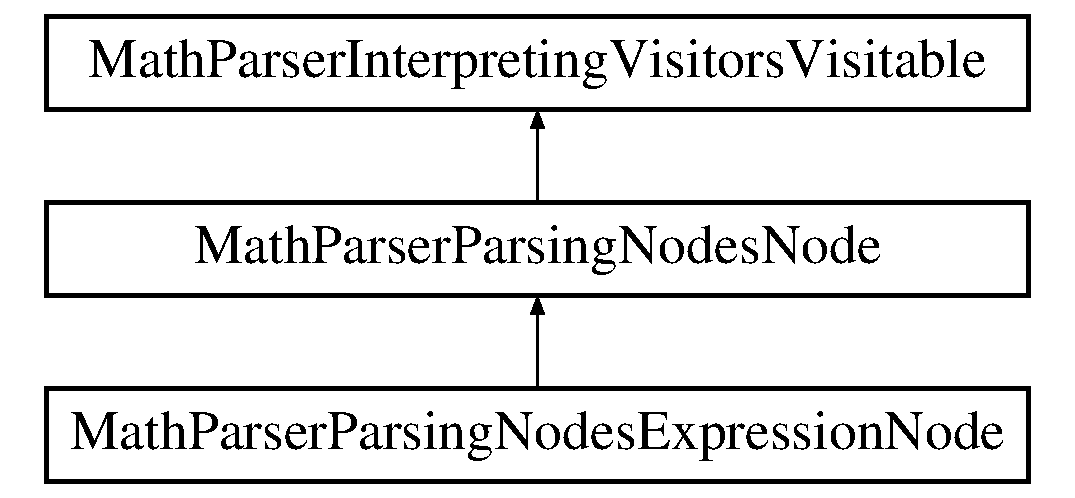
\includegraphics[height=3.000000cm]{classMathParser_1_1Parsing_1_1Nodes_1_1ExpressionNode}
\end{center}
\end{figure}
\subsection*{Public Member Functions}
\begin{DoxyCompactItemize}
\item 
\hyperlink{classMathParser_1_1Parsing_1_1Nodes_1_1ExpressionNode_ad225055b7e075eabc33c0f7bfd4253cb}{\-\_\-\-\_\-construct} (\$left, \$operator=null, \$right=null)
\begin{DoxyCompactList}\small\item\em Constructor. \end{DoxyCompactList}\item 
\hyperlink{classMathParser_1_1Parsing_1_1Nodes_1_1ExpressionNode_a8e50a23c59679015c5e45b723d7bcb7d}{get\-Left} ()
\begin{DoxyCompactList}\small\item\em Return the first (left) operand. \end{DoxyCompactList}\item 
\hyperlink{classMathParser_1_1Parsing_1_1Nodes_1_1ExpressionNode_afeb588203d9912983be68c68aaad8a87}{get\-Operator} ()
\begin{DoxyCompactList}\small\item\em Return the operator. \end{DoxyCompactList}\item 
\hyperlink{classMathParser_1_1Parsing_1_1Nodes_1_1ExpressionNode_af0a80f6914435eee930199efb29579dd}{get\-Right} ()
\begin{DoxyCompactList}\small\item\em Return the second (right) operand. \end{DoxyCompactList}\item 
\hypertarget{classMathParser_1_1Parsing_1_1Nodes_1_1ExpressionNode_a3794b9185ed7928df1f39ec42c557106}{\hyperlink{classMathParser_1_1Parsing_1_1Nodes_1_1ExpressionNode_a3794b9185ed7928df1f39ec42c557106}{accept} (\hyperlink{interfaceMathParser_1_1Interpreting_1_1Visitors_1_1Visitor}{Visitor} \$visitor)}\label{classMathParser_1_1Parsing_1_1Nodes_1_1ExpressionNode_a3794b9185ed7928df1f39ec42c557106}

\begin{DoxyCompactList}\small\item\em Implementing the Visitable interface. \end{DoxyCompactList}\end{DoxyCompactItemize}
\subsection*{Private Attributes}
\begin{DoxyCompactItemize}
\item 
\hypertarget{classMathParser_1_1Parsing_1_1Nodes_1_1ExpressionNode_ace203efd9b7ea8833a23378f6ab4f084}{{\bfseries \$left}}\label{classMathParser_1_1Parsing_1_1Nodes_1_1ExpressionNode_ace203efd9b7ea8833a23378f6ab4f084}

\item 
\hypertarget{classMathParser_1_1Parsing_1_1Nodes_1_1ExpressionNode_ad98a4daf07ef12dccb13598f2d6e0d8c}{{\bfseries \$operator}}\label{classMathParser_1_1Parsing_1_1Nodes_1_1ExpressionNode_ad98a4daf07ef12dccb13598f2d6e0d8c}

\item 
\hypertarget{classMathParser_1_1Parsing_1_1Nodes_1_1ExpressionNode_a6698fe89d391cd7b7dc84e4f1a06d2f4}{{\bfseries \$right}}\label{classMathParser_1_1Parsing_1_1Nodes_1_1ExpressionNode_a6698fe89d391cd7b7dc84e4f1a06d2f4}

\end{DoxyCompactItemize}
\subsection*{Additional Inherited Members}


\subsection{Detailed Description}
A\-S\-T node representing a binary operator. 

\subsection{Constructor \& Destructor Documentation}
\hypertarget{classMathParser_1_1Parsing_1_1Nodes_1_1ExpressionNode_ad225055b7e075eabc33c0f7bfd4253cb}{\index{Math\-Parser\-::\-Parsing\-::\-Nodes\-::\-Expression\-Node@{Math\-Parser\-::\-Parsing\-::\-Nodes\-::\-Expression\-Node}!\-\_\-\-\_\-construct@{\-\_\-\-\_\-construct}}
\index{\-\_\-\-\_\-construct@{\-\_\-\-\_\-construct}!MathParser::Parsing::Nodes::ExpressionNode@{Math\-Parser\-::\-Parsing\-::\-Nodes\-::\-Expression\-Node}}
\subsubsection[{\-\_\-\-\_\-construct}]{\setlength{\rightskip}{0pt plus 5cm}Math\-Parser\textbackslash{}\-Parsing\textbackslash{}\-Nodes\textbackslash{}\-Expression\-Node\-::\-\_\-\-\_\-construct (
\begin{DoxyParamCaption}
\item[{}]{\$left, }
\item[{}]{\$operator = {\ttfamily null}, }
\item[{}]{\$right = {\ttfamily null}}
\end{DoxyParamCaption}
)}}\label{classMathParser_1_1Parsing_1_1Nodes_1_1ExpressionNode_ad225055b7e075eabc33c0f7bfd4253cb}


Constructor. 

Construct a binary operator node from (one or) two operands and an operator.

For convenience, the constructor accept int or float as operands, automatically converting these to Number\-Nodes


\begin{DoxyParams}[1]{Parameters}
\hyperlink{classMathParser_1_1Parsing_1_1Nodes_1_1Node}{Node} | null | int | float & {\em \$left} & First operand \\
\hline
 & {\em string} & operator Name of operator \\
\hline
\hyperlink{classMathParser_1_1Parsing_1_1Nodes_1_1Node}{Node} | null | int | float & {\em \$right} & Second operand \\
\hline
\end{DoxyParams}


\subsection{Member Function Documentation}
\hypertarget{classMathParser_1_1Parsing_1_1Nodes_1_1ExpressionNode_a8e50a23c59679015c5e45b723d7bcb7d}{\index{Math\-Parser\-::\-Parsing\-::\-Nodes\-::\-Expression\-Node@{Math\-Parser\-::\-Parsing\-::\-Nodes\-::\-Expression\-Node}!get\-Left@{get\-Left}}
\index{get\-Left@{get\-Left}!MathParser::Parsing::Nodes::ExpressionNode@{Math\-Parser\-::\-Parsing\-::\-Nodes\-::\-Expression\-Node}}
\subsubsection[{get\-Left}]{\setlength{\rightskip}{0pt plus 5cm}Math\-Parser\textbackslash{}\-Parsing\textbackslash{}\-Nodes\textbackslash{}\-Expression\-Node\-::get\-Left (
\begin{DoxyParamCaption}
{}
\end{DoxyParamCaption}
)}}\label{classMathParser_1_1Parsing_1_1Nodes_1_1ExpressionNode_a8e50a23c59679015c5e45b723d7bcb7d}


Return the first (left) operand. 


\begin{DoxyRetVals}{Return values}
{\em Node$\vert$null} & \\
\hline
\end{DoxyRetVals}
\hypertarget{classMathParser_1_1Parsing_1_1Nodes_1_1ExpressionNode_afeb588203d9912983be68c68aaad8a87}{\index{Math\-Parser\-::\-Parsing\-::\-Nodes\-::\-Expression\-Node@{Math\-Parser\-::\-Parsing\-::\-Nodes\-::\-Expression\-Node}!get\-Operator@{get\-Operator}}
\index{get\-Operator@{get\-Operator}!MathParser::Parsing::Nodes::ExpressionNode@{Math\-Parser\-::\-Parsing\-::\-Nodes\-::\-Expression\-Node}}
\subsubsection[{get\-Operator}]{\setlength{\rightskip}{0pt plus 5cm}Math\-Parser\textbackslash{}\-Parsing\textbackslash{}\-Nodes\textbackslash{}\-Expression\-Node\-::get\-Operator (
\begin{DoxyParamCaption}
{}
\end{DoxyParamCaption}
)}}\label{classMathParser_1_1Parsing_1_1Nodes_1_1ExpressionNode_afeb588203d9912983be68c68aaad8a87}


Return the operator. 


\begin{DoxyRetVals}{Return values}
{\em string} & \\
\hline
\end{DoxyRetVals}
\hypertarget{classMathParser_1_1Parsing_1_1Nodes_1_1ExpressionNode_af0a80f6914435eee930199efb29579dd}{\index{Math\-Parser\-::\-Parsing\-::\-Nodes\-::\-Expression\-Node@{Math\-Parser\-::\-Parsing\-::\-Nodes\-::\-Expression\-Node}!get\-Right@{get\-Right}}
\index{get\-Right@{get\-Right}!MathParser::Parsing::Nodes::ExpressionNode@{Math\-Parser\-::\-Parsing\-::\-Nodes\-::\-Expression\-Node}}
\subsubsection[{get\-Right}]{\setlength{\rightskip}{0pt plus 5cm}Math\-Parser\textbackslash{}\-Parsing\textbackslash{}\-Nodes\textbackslash{}\-Expression\-Node\-::get\-Right (
\begin{DoxyParamCaption}
{}
\end{DoxyParamCaption}
)}}\label{classMathParser_1_1Parsing_1_1Nodes_1_1ExpressionNode_af0a80f6914435eee930199efb29579dd}


Return the second (right) operand. 


\begin{DoxyRetVals}{Return values}
{\em Node$\vert$null} & \\
\hline
\end{DoxyRetVals}


The documentation for this class was generated from the following file\-:\begin{DoxyCompactItemize}
\item 
src/\-Math\-Parser/\-Parsing/\-Nodes/Expression\-Node.\-php\end{DoxyCompactItemize}

\hypertarget{classMathParser_1_1Parsing_1_1Nodes_1_1FunctionNode}{\section{Math\-Parser\textbackslash{}Parsing\textbackslash{}Nodes\textbackslash{}Function\-Node Class Reference}
\label{classMathParser_1_1Parsing_1_1Nodes_1_1FunctionNode}\index{Math\-Parser\textbackslash{}\-Parsing\textbackslash{}\-Nodes\textbackslash{}\-Function\-Node@{Math\-Parser\textbackslash{}\-Parsing\textbackslash{}\-Nodes\textbackslash{}\-Function\-Node}}
}


A\-S\-T node representing a function applications (e.\-g.  


Inheritance diagram for Math\-Parser\textbackslash{}Parsing\textbackslash{}Nodes\textbackslash{}Function\-Node\-:\begin{figure}[H]
\begin{center}
\leavevmode
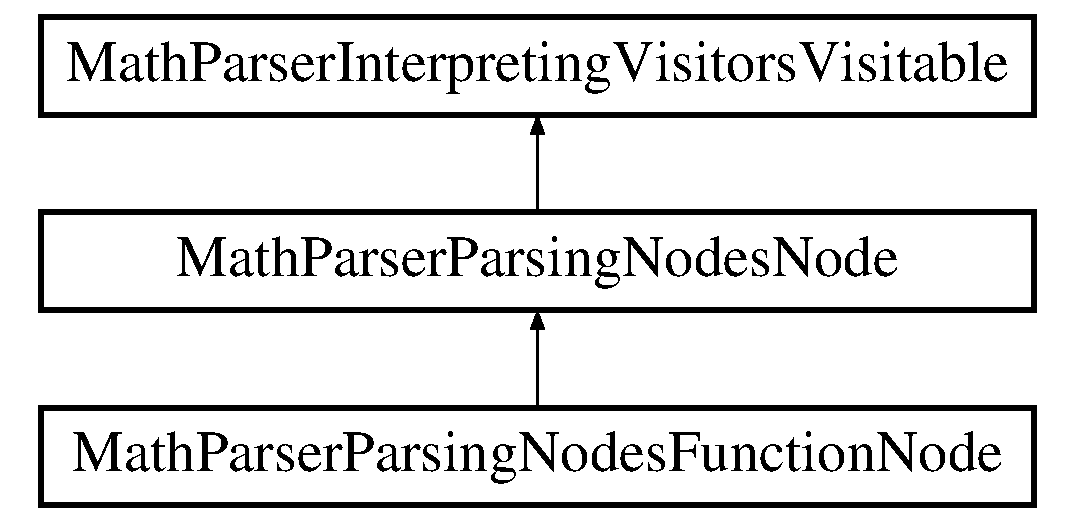
\includegraphics[height=3.000000cm]{classMathParser_1_1Parsing_1_1Nodes_1_1FunctionNode}
\end{center}
\end{figure}
\subsection*{Public Member Functions}
\begin{DoxyCompactItemize}
\item 
\hypertarget{classMathParser_1_1Parsing_1_1Nodes_1_1FunctionNode_a1e5f029d0dbac72b28d6d42048140b3b}{{\bfseries \-\_\-\-\_\-construct} (\$name, \$operand)}\label{classMathParser_1_1Parsing_1_1Nodes_1_1FunctionNode_a1e5f029d0dbac72b28d6d42048140b3b}

\item 
\hyperlink{classMathParser_1_1Parsing_1_1Nodes_1_1FunctionNode_a797c638dc3ef116100b5db449e7fb231}{get\-Name} ()
\begin{DoxyCompactList}\small\item\em Return the name of the function. \end{DoxyCompactList}\item 
\hyperlink{classMathParser_1_1Parsing_1_1Nodes_1_1FunctionNode_acea27b2dadadaa202ddefb69fb3a2cdf}{get\-Operand} ()
\begin{DoxyCompactList}\small\item\em Return the operand. \end{DoxyCompactList}\item 
\hypertarget{classMathParser_1_1Parsing_1_1Nodes_1_1FunctionNode_a9796a0fdaf49525adc9ea539b4291835}{\hyperlink{classMathParser_1_1Parsing_1_1Nodes_1_1FunctionNode_a9796a0fdaf49525adc9ea539b4291835}{accept} (\hyperlink{interfaceMathParser_1_1Interpreting_1_1Visitors_1_1Visitor}{Visitor} \$visitor)}\label{classMathParser_1_1Parsing_1_1Nodes_1_1FunctionNode_a9796a0fdaf49525adc9ea539b4291835}

\begin{DoxyCompactList}\small\item\em Implementing the Visitable interface. \end{DoxyCompactList}\end{DoxyCompactItemize}
\subsection*{Private Attributes}
\begin{DoxyCompactItemize}
\item 
\hypertarget{classMathParser_1_1Parsing_1_1Nodes_1_1FunctionNode_abc812043d66ed2e415f6cb79bb596be3}{{\bfseries \$name}}\label{classMathParser_1_1Parsing_1_1Nodes_1_1FunctionNode_abc812043d66ed2e415f6cb79bb596be3}

\item 
\hypertarget{classMathParser_1_1Parsing_1_1Nodes_1_1FunctionNode_aef940f5b536e7e370eef241088522331}{{\bfseries \$operand}}\label{classMathParser_1_1Parsing_1_1Nodes_1_1FunctionNode_aef940f5b536e7e370eef241088522331}

\end{DoxyCompactItemize}
\subsection*{Additional Inherited Members}


\subsection{Detailed Description}
A\-S\-T node representing a function applications (e.\-g. 

sin(...)) 

\subsection{Member Function Documentation}
\hypertarget{classMathParser_1_1Parsing_1_1Nodes_1_1FunctionNode_a797c638dc3ef116100b5db449e7fb231}{\index{Math\-Parser\-::\-Parsing\-::\-Nodes\-::\-Function\-Node@{Math\-Parser\-::\-Parsing\-::\-Nodes\-::\-Function\-Node}!get\-Name@{get\-Name}}
\index{get\-Name@{get\-Name}!MathParser::Parsing::Nodes::FunctionNode@{Math\-Parser\-::\-Parsing\-::\-Nodes\-::\-Function\-Node}}
\subsubsection[{get\-Name}]{\setlength{\rightskip}{0pt plus 5cm}Math\-Parser\textbackslash{}\-Parsing\textbackslash{}\-Nodes\textbackslash{}\-Function\-Node\-::get\-Name (
\begin{DoxyParamCaption}
{}
\end{DoxyParamCaption}
)}}\label{classMathParser_1_1Parsing_1_1Nodes_1_1FunctionNode_a797c638dc3ef116100b5db449e7fb231}


Return the name of the function. 


\begin{DoxyRetVals}{Return values}
{\em string} & \\
\hline
\end{DoxyRetVals}
\hypertarget{classMathParser_1_1Parsing_1_1Nodes_1_1FunctionNode_acea27b2dadadaa202ddefb69fb3a2cdf}{\index{Math\-Parser\-::\-Parsing\-::\-Nodes\-::\-Function\-Node@{Math\-Parser\-::\-Parsing\-::\-Nodes\-::\-Function\-Node}!get\-Operand@{get\-Operand}}
\index{get\-Operand@{get\-Operand}!MathParser::Parsing::Nodes::FunctionNode@{Math\-Parser\-::\-Parsing\-::\-Nodes\-::\-Function\-Node}}
\subsubsection[{get\-Operand}]{\setlength{\rightskip}{0pt plus 5cm}Math\-Parser\textbackslash{}\-Parsing\textbackslash{}\-Nodes\textbackslash{}\-Function\-Node\-::get\-Operand (
\begin{DoxyParamCaption}
{}
\end{DoxyParamCaption}
)}}\label{classMathParser_1_1Parsing_1_1Nodes_1_1FunctionNode_acea27b2dadadaa202ddefb69fb3a2cdf}


Return the operand. 


\begin{DoxyRetVals}{Return values}
{\em \hyperlink{classMathParser_1_1Parsing_1_1Nodes_1_1Node}{Node}} & \\
\hline
\end{DoxyRetVals}


The documentation for this class was generated from the following file\-:\begin{DoxyCompactItemize}
\item 
src/\-Math\-Parser/\-Parsing/\-Nodes/Function\-Node.\-php\end{DoxyCompactItemize}

\hypertarget{classMathParser_1_1Interpreting_1_1LaTeXPrinter}{\section{Math\-Parser\textbackslash{}Interpreting\textbackslash{}La\-Te\-X\-Printer Class Reference}
\label{classMathParser_1_1Interpreting_1_1LaTeXPrinter}\index{Math\-Parser\textbackslash{}\-Interpreting\textbackslash{}\-La\-Te\-X\-Printer@{Math\-Parser\textbackslash{}\-Interpreting\textbackslash{}\-La\-Te\-X\-Printer}}
}


Create La\-Te\-X code for prettyprinting a mathematical expression (for example via Math\-Jax)  


Inheritance diagram for Math\-Parser\textbackslash{}Interpreting\textbackslash{}La\-Te\-X\-Printer\-:\begin{figure}[H]
\begin{center}
\leavevmode
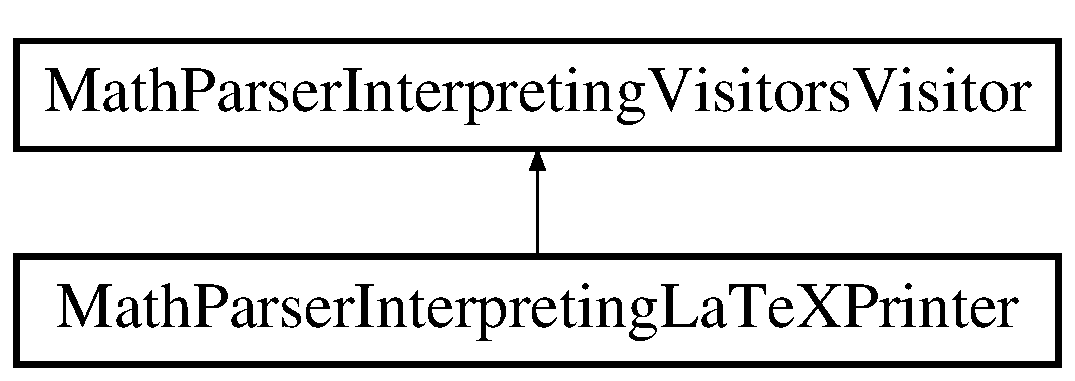
\includegraphics[height=2.000000cm]{classMathParser_1_1Interpreting_1_1LaTeXPrinter}
\end{center}
\end{figure}
\subsection*{Public Member Functions}
\begin{DoxyCompactItemize}
\item 
\hyperlink{classMathParser_1_1Interpreting_1_1LaTeXPrinter_a68bcaa8f65dbebd8aadd6002b50dea49}{visit\-Expression\-Node} (\hyperlink{classMathParser_1_1Parsing_1_1Nodes_1_1ExpressionNode}{Expression\-Node} \$node)
\begin{DoxyCompactList}\small\item\em Generate La\-Te\-X code for an Expression\-Node. \end{DoxyCompactList}\item 
\hyperlink{classMathParser_1_1Interpreting_1_1LaTeXPrinter_a5bbb40a11601dc347c9d4ec629723396}{visit\-Number\-Node} (\hyperlink{classMathParser_1_1Parsing_1_1Nodes_1_1NumberNode}{Number\-Node} \$node)
\begin{DoxyCompactList}\small\item\em Generate La\-Te\-X code for a Number\-Node. \end{DoxyCompactList}\item 
\hyperlink{classMathParser_1_1Interpreting_1_1LaTeXPrinter_aced38823c7de0b9ad84884028370a8d2}{visit\-Variable\-Node} (\hyperlink{classMathParser_1_1Parsing_1_1Nodes_1_1VariableNode}{Variable\-Node} \$node)
\begin{DoxyCompactList}\small\item\em Generate La\-Te\-X code for a Variable\-Node. \end{DoxyCompactList}\item 
\hyperlink{classMathParser_1_1Interpreting_1_1LaTeXPrinter_a85eb667103f7b04abfe3c83e6c0e24a2}{visit\-Function\-Node} (\hyperlink{classMathParser_1_1Parsing_1_1Nodes_1_1FunctionNode}{Function\-Node} \$node)
\begin{DoxyCompactList}\small\item\em Generate La\-Te\-X code for a Function\-Node. \end{DoxyCompactList}\item 
\hyperlink{classMathParser_1_1Interpreting_1_1LaTeXPrinter_aaa2c3cfcfa01461f52a8f656ef52b92c}{visit\-Constant\-Node} (\hyperlink{classMathParser_1_1Parsing_1_1Nodes_1_1ConstantNode}{Constant\-Node} \$node)
\begin{DoxyCompactList}\small\item\em Generate La\-Te\-X code for a Constant\-Node. \end{DoxyCompactList}\item 
\hyperlink{classMathParser_1_1Interpreting_1_1LaTeXPrinter_a0155571b5b4fea8a6b762beabdb02ccf}{parenthesize} (\hyperlink{classMathParser_1_1Parsing_1_1Nodes_1_1Node}{Node} \$node, \$cutoff='$\ast$', \$add\-Space=false)
\begin{DoxyCompactList}\small\item\em Add parentheses to the La\-Te\-X representation of \$node if needed. \end{DoxyCompactList}\item 
\hyperlink{classMathParser_1_1Interpreting_1_1LaTeXPrinter_a0f7cfa301dbab484b82a4aa83e9a37f1}{braces\-Needed} (\hyperlink{classMathParser_1_1Parsing_1_1Nodes_1_1Node}{Node} \$node)
\begin{DoxyCompactList}\small\item\em Add curly braces around the La\-Tex representation of \$node if needed. \end{DoxyCompactList}\end{DoxyCompactItemize}
\subsection*{Private Attributes}
\begin{DoxyCompactItemize}
\item 
\hypertarget{classMathParser_1_1Interpreting_1_1LaTeXPrinter_ad3c7631e73a252a1920dab0825b0be30}{{\bfseries \$lexer}}\label{classMathParser_1_1Interpreting_1_1LaTeXPrinter_ad3c7631e73a252a1920dab0825b0be30}

\end{DoxyCompactItemize}


\subsection{Detailed Description}
Create La\-Te\-X code for prettyprinting a mathematical expression (for example via Math\-Jax) 

Implementation of a Visitor, transforming an A\-S\-T into a string giving La\-Te\-X code for the expression.

The class in general does {\itshape not} generate the best possible La\-Te\-X code, and needs more work to be used in a production setting.

\subsubsection*{Example\-:}


\begin{DoxyCode}
$parser = \textcolor{keyword}{new} StdMathParser();
$f = $parser->parse(\textcolor{stringliteral}{'exp(2x)+xy'});
printer = \textcolor{keyword}{new} LaTeXPrinter();
result = $f->accept($printer);    \textcolor{comment}{// Generates "e^\{2x\}+xy"}
\end{DoxyCode}


Note that surrounding {\ttfamily \$}, {\ttfamily \$\$} or {\ttfamily \textbackslash{}begin\{equation\}..\textbackslash{}end\{equation\}} has to be added manually. 

\subsection{Member Function Documentation}
\hypertarget{classMathParser_1_1Interpreting_1_1LaTeXPrinter_a0f7cfa301dbab484b82a4aa83e9a37f1}{\index{Math\-Parser\-::\-Interpreting\-::\-La\-Te\-X\-Printer@{Math\-Parser\-::\-Interpreting\-::\-La\-Te\-X\-Printer}!braces\-Needed@{braces\-Needed}}
\index{braces\-Needed@{braces\-Needed}!MathParser::Interpreting::LaTeXPrinter@{Math\-Parser\-::\-Interpreting\-::\-La\-Te\-X\-Printer}}
\subsubsection[{braces\-Needed}]{\setlength{\rightskip}{0pt plus 5cm}Math\-Parser\textbackslash{}\-Interpreting\textbackslash{}\-La\-Te\-X\-Printer\-::braces\-Needed (
\begin{DoxyParamCaption}
\item[{{\bf Node}}]{\$node}
\end{DoxyParamCaption}
)}}\label{classMathParser_1_1Interpreting_1_1LaTeXPrinter_a0f7cfa301dbab484b82a4aa83e9a37f1}


Add curly braces around the La\-Tex representation of \$node if needed. 

Nodes representing a single Constant\-Node, Variable\-Node or Number\-Nodes (0--9) are returned as-\/is. Other Nodes get curly braces around their La\-Te\-X code.


\begin{DoxyParams}[1]{Parameters}
Node & {\em \$node} & A\-S\-T to parse \\
\hline
\end{DoxyParams}

\begin{DoxyRetVals}{Return values}
{\em string} & \\
\hline
\end{DoxyRetVals}
\hypertarget{classMathParser_1_1Interpreting_1_1LaTeXPrinter_a0155571b5b4fea8a6b762beabdb02ccf}{\index{Math\-Parser\-::\-Interpreting\-::\-La\-Te\-X\-Printer@{Math\-Parser\-::\-Interpreting\-::\-La\-Te\-X\-Printer}!parenthesize@{parenthesize}}
\index{parenthesize@{parenthesize}!MathParser::Interpreting::LaTeXPrinter@{Math\-Parser\-::\-Interpreting\-::\-La\-Te\-X\-Printer}}
\subsubsection[{parenthesize}]{\setlength{\rightskip}{0pt plus 5cm}Math\-Parser\textbackslash{}\-Interpreting\textbackslash{}\-La\-Te\-X\-Printer\-::parenthesize (
\begin{DoxyParamCaption}
\item[{{\bf Node}}]{\$node, }
\item[{}]{\$cutoff = {\ttfamily '$\ast$'}, }
\item[{}]{\$add\-Space = {\ttfamily false}}
\end{DoxyParamCaption}
)}}\label{classMathParser_1_1Interpreting_1_1LaTeXPrinter_a0155571b5b4fea8a6b762beabdb02ccf}


Add parentheses to the La\-Te\-X representation of \$node if needed. 


\begin{DoxyParams}[1]{Parameters}
Node & {\em \$node} & The A\-S\-T to typeset \\
\hline
string & {\em \$cutoff} & A token representing the precedence of the parent node. Operands with a lower precedence have parentheses added. \\
\hline
bool & {\em \$add\-Space} & Flag determining whether an additional space should be added at the beginning of the returned string. \\
\hline
\end{DoxyParams}

\begin{DoxyRetVals}{Return values}
{\em string} & \\
\hline
\end{DoxyRetVals}
\hypertarget{classMathParser_1_1Interpreting_1_1LaTeXPrinter_aaa2c3cfcfa01461f52a8f656ef52b92c}{\index{Math\-Parser\-::\-Interpreting\-::\-La\-Te\-X\-Printer@{Math\-Parser\-::\-Interpreting\-::\-La\-Te\-X\-Printer}!visit\-Constant\-Node@{visit\-Constant\-Node}}
\index{visit\-Constant\-Node@{visit\-Constant\-Node}!MathParser::Interpreting::LaTeXPrinter@{Math\-Parser\-::\-Interpreting\-::\-La\-Te\-X\-Printer}}
\subsubsection[{visit\-Constant\-Node}]{\setlength{\rightskip}{0pt plus 5cm}Math\-Parser\textbackslash{}\-Interpreting\textbackslash{}\-La\-Te\-X\-Printer\-::visit\-Constant\-Node (
\begin{DoxyParamCaption}
\item[{{\bf Constant\-Node}}]{\$node}
\end{DoxyParamCaption}
)}}\label{classMathParser_1_1Interpreting_1_1LaTeXPrinter_aaa2c3cfcfa01461f52a8f656ef52b92c}


Generate La\-Te\-X code for a Constant\-Node. 

Create a string giving La\-Te\-X code for a Constant\-Node. {\ttfamily pi} typesets as {\ttfamily \textbackslash{}pi} and {\ttfamily e} simply as {\ttfamily e}.


\begin{DoxyExceptions}{Exceptions}
{\em Unknown\-Constant\-Exception} & for nodes representing other constants. \\
\hline
\end{DoxyExceptions}

\begin{DoxyParams}[1]{Parameters}
Constant\-Node & {\em \$node} & A\-S\-T to be typeset \\
\hline
\end{DoxyParams}

\begin{DoxyRetVals}{Return values}
{\em string} & \\
\hline
\end{DoxyRetVals}


Implements \hyperlink{interfaceMathParser_1_1Interpreting_1_1Visitors_1_1Visitor_ac694089225b20c9f848bcfb0a5e600f0}{Math\-Parser\textbackslash{}\-Interpreting\textbackslash{}\-Visitors\textbackslash{}\-Visitor}.

\hypertarget{classMathParser_1_1Interpreting_1_1LaTeXPrinter_a68bcaa8f65dbebd8aadd6002b50dea49}{\index{Math\-Parser\-::\-Interpreting\-::\-La\-Te\-X\-Printer@{Math\-Parser\-::\-Interpreting\-::\-La\-Te\-X\-Printer}!visit\-Expression\-Node@{visit\-Expression\-Node}}
\index{visit\-Expression\-Node@{visit\-Expression\-Node}!MathParser::Interpreting::LaTeXPrinter@{Math\-Parser\-::\-Interpreting\-::\-La\-Te\-X\-Printer}}
\subsubsection[{visit\-Expression\-Node}]{\setlength{\rightskip}{0pt plus 5cm}Math\-Parser\textbackslash{}\-Interpreting\textbackslash{}\-La\-Te\-X\-Printer\-::visit\-Expression\-Node (
\begin{DoxyParamCaption}
\item[{{\bf Expression\-Node}}]{\$node}
\end{DoxyParamCaption}
)}}\label{classMathParser_1_1Interpreting_1_1LaTeXPrinter_a68bcaa8f65dbebd8aadd6002b50dea49}


Generate La\-Te\-X code for an Expression\-Node. 

Create a string giving La\-Te\-X code for an Expression\-Node {\ttfamily (x op y)} where {\ttfamily op} is one of {\ttfamily +}, {\ttfamily -\/}, {\ttfamily $\ast$}, {\ttfamily /} or {\ttfamily $^\wedge$}

\paragraph*{Typesetting rules\-:}


\begin{DoxyItemize}
\item Adds parantheses around each operand, if needed. (I.\-e. if their precedence lower than that of the current Node.) For example, the A\-S\-T {\ttfamily ($^\wedge$ (+ 1 2) 3)} generates {\ttfamily (1+2)$^\wedge$3} but {\ttfamily (+ ($^\wedge$ 1 2) 3)} generates {\ttfamily 1$^\wedge$2+3} as expected.
\item Multiplications are typeset implicitly {\ttfamily ($\ast$ x y)} returns {\ttfamily xy} or using {\ttfamily \textbackslash{}cdot} if the first factor is a Function\-Node or the (left operand) in the second factor is a Number\-Node, so {\ttfamily ($\ast$ x 2)} return {\ttfamily x \textbackslash{}cdot 2} and {\ttfamily ($\ast$ (sin x) x)} return {\ttfamily \textbackslash{}sin x \textbackslash{}cdot x} (but {\ttfamily ($\ast$ x (sin x))} returns {\ttfamily x\textbackslash{}sin x})
\item Divisions are typeset using {\ttfamily \textbackslash{}frac}
\item Exponentiation adds braces around the power when needed.
\end{DoxyItemize}


\begin{DoxyParams}[1]{Parameters}
Expression\-Node & {\em \$node} & A\-S\-T to be typeset \\
\hline
\end{DoxyParams}

\begin{DoxyRetVals}{Return values}
{\em string} & \\
\hline
\end{DoxyRetVals}


Implements \hyperlink{interfaceMathParser_1_1Interpreting_1_1Visitors_1_1Visitor_a201489f6ae0ccc3c25ff153a57994fa1}{Math\-Parser\textbackslash{}\-Interpreting\textbackslash{}\-Visitors\textbackslash{}\-Visitor}.

\hypertarget{classMathParser_1_1Interpreting_1_1LaTeXPrinter_a85eb667103f7b04abfe3c83e6c0e24a2}{\index{Math\-Parser\-::\-Interpreting\-::\-La\-Te\-X\-Printer@{Math\-Parser\-::\-Interpreting\-::\-La\-Te\-X\-Printer}!visit\-Function\-Node@{visit\-Function\-Node}}
\index{visit\-Function\-Node@{visit\-Function\-Node}!MathParser::Interpreting::LaTeXPrinter@{Math\-Parser\-::\-Interpreting\-::\-La\-Te\-X\-Printer}}
\subsubsection[{visit\-Function\-Node}]{\setlength{\rightskip}{0pt plus 5cm}Math\-Parser\textbackslash{}\-Interpreting\textbackslash{}\-La\-Te\-X\-Printer\-::visit\-Function\-Node (
\begin{DoxyParamCaption}
\item[{{\bf Function\-Node}}]{\$node}
\end{DoxyParamCaption}
)}}\label{classMathParser_1_1Interpreting_1_1LaTeXPrinter_a85eb667103f7b04abfe3c83e6c0e24a2}


Generate La\-Te\-X code for a Function\-Node. 

Create a string giving La\-Te\-X code for a function\-Node.

\paragraph*{Typesetting rules\-:}


\begin{DoxyItemize}
\item {\ttfamily sqrt(op)} is typeset as {\ttfamily \textbackslash{}sqrt\{op\} -\/}exp(op){\ttfamily is either typeset as}e$^\wedge$\{op\}{\ttfamily , if}op{\ttfamily is a simple expression or as}(op)` for more complicated operands.
\end{DoxyItemize}

T\-O\-D\-O Non-\/standard functions should be typeset using  
\begin{DoxyParams}[1]{Parameters}
Function\-Node & {\em \$node} & A\-S\-T to be typeset \\
\hline
\end{DoxyParams}

\begin{DoxyRetVals}{Return values}
{\em string} & \\
\hline
\end{DoxyRetVals}


Implements \hyperlink{interfaceMathParser_1_1Interpreting_1_1Visitors_1_1Visitor_a497e4a990f99689616c25e76b0ec6ef1}{Math\-Parser\textbackslash{}\-Interpreting\textbackslash{}\-Visitors\textbackslash{}\-Visitor}.

\hypertarget{classMathParser_1_1Interpreting_1_1LaTeXPrinter_a5bbb40a11601dc347c9d4ec629723396}{\index{Math\-Parser\-::\-Interpreting\-::\-La\-Te\-X\-Printer@{Math\-Parser\-::\-Interpreting\-::\-La\-Te\-X\-Printer}!visit\-Number\-Node@{visit\-Number\-Node}}
\index{visit\-Number\-Node@{visit\-Number\-Node}!MathParser::Interpreting::LaTeXPrinter@{Math\-Parser\-::\-Interpreting\-::\-La\-Te\-X\-Printer}}
\subsubsection[{visit\-Number\-Node}]{\setlength{\rightskip}{0pt plus 5cm}Math\-Parser\textbackslash{}\-Interpreting\textbackslash{}\-La\-Te\-X\-Printer\-::visit\-Number\-Node (
\begin{DoxyParamCaption}
\item[{{\bf Number\-Node}}]{\$node}
\end{DoxyParamCaption}
)}}\label{classMathParser_1_1Interpreting_1_1LaTeXPrinter_a5bbb40a11601dc347c9d4ec629723396}


Generate La\-Te\-X code for a Number\-Node. 

Create a string giving La\-Te\-X code for a Number\-Node. Currently, there is no special formatting of numbers.


\begin{DoxyParams}[1]{Parameters}
Number\-Node & {\em \$node} & A\-S\-T to be typeset \\
\hline
\end{DoxyParams}

\begin{DoxyRetVals}{Return values}
{\em string} & \\
\hline
\end{DoxyRetVals}


Implements \hyperlink{interfaceMathParser_1_1Interpreting_1_1Visitors_1_1Visitor_acbcd1cbecf76ba51c893a49746162dc1}{Math\-Parser\textbackslash{}\-Interpreting\textbackslash{}\-Visitors\textbackslash{}\-Visitor}.

\hypertarget{classMathParser_1_1Interpreting_1_1LaTeXPrinter_aced38823c7de0b9ad84884028370a8d2}{\index{Math\-Parser\-::\-Interpreting\-::\-La\-Te\-X\-Printer@{Math\-Parser\-::\-Interpreting\-::\-La\-Te\-X\-Printer}!visit\-Variable\-Node@{visit\-Variable\-Node}}
\index{visit\-Variable\-Node@{visit\-Variable\-Node}!MathParser::Interpreting::LaTeXPrinter@{Math\-Parser\-::\-Interpreting\-::\-La\-Te\-X\-Printer}}
\subsubsection[{visit\-Variable\-Node}]{\setlength{\rightskip}{0pt plus 5cm}Math\-Parser\textbackslash{}\-Interpreting\textbackslash{}\-La\-Te\-X\-Printer\-::visit\-Variable\-Node (
\begin{DoxyParamCaption}
\item[{{\bf Variable\-Node}}]{\$node}
\end{DoxyParamCaption}
)}}\label{classMathParser_1_1Interpreting_1_1LaTeXPrinter_aced38823c7de0b9ad84884028370a8d2}


Generate La\-Te\-X code for a Variable\-Node. 

Create a string giving La\-Te\-X code for a Variable\-Node. Currently, there is no special formatting of variables.


\begin{DoxyParams}[1]{Parameters}
Variable\-Node & {\em \$node} & A\-S\-T to be typeset \\
\hline
\end{DoxyParams}

\begin{DoxyRetVals}{Return values}
{\em string} & \\
\hline
\end{DoxyRetVals}


Implements \hyperlink{interfaceMathParser_1_1Interpreting_1_1Visitors_1_1Visitor_a292630a7204dadd96877d8182f38deb0}{Math\-Parser\textbackslash{}\-Interpreting\textbackslash{}\-Visitors\textbackslash{}\-Visitor}.



The documentation for this class was generated from the following file\-:\begin{DoxyCompactItemize}
\item 
src/\-Math\-Parser/\-Interpreting/La\-Te\-X\-Printer.\-php\end{DoxyCompactItemize}

\hypertarget{classMathParser_1_1Lexing_1_1Lexer}{\section{Math\-Parser\textbackslash{}Lexing\textbackslash{}Lexer Class Reference}
\label{classMathParser_1_1Lexing_1_1Lexer}\index{Math\-Parser\textbackslash{}\-Lexing\textbackslash{}\-Lexer@{Math\-Parser\textbackslash{}\-Lexing\textbackslash{}\-Lexer}}
}


Generic very simple lexer, capable of matching tokens defined by regular expressions.  


Inheritance diagram for Math\-Parser\textbackslash{}Lexing\textbackslash{}Lexer\-:\begin{figure}[H]
\begin{center}
\leavevmode
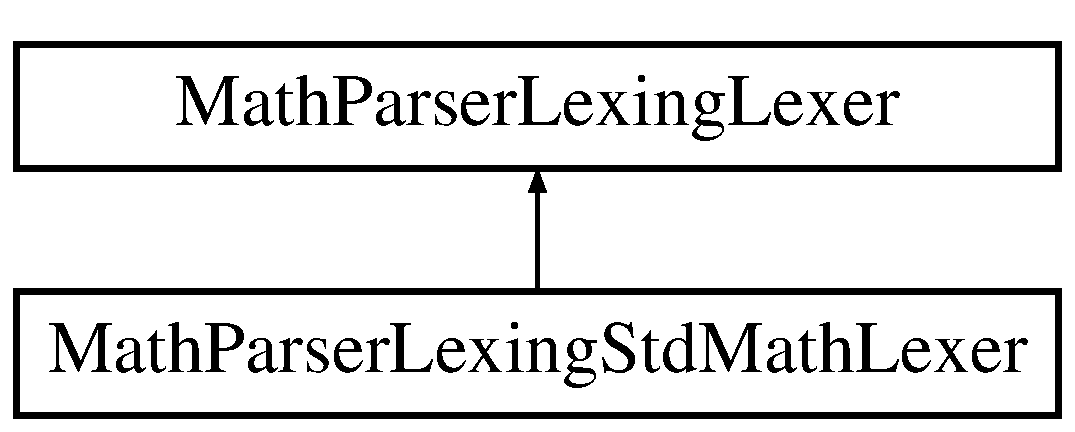
\includegraphics[height=2.000000cm]{classMathParser_1_1Lexing_1_1Lexer}
\end{center}
\end{figure}
\subsection*{Public Member Functions}
\begin{DoxyCompactItemize}
\item 
\hyperlink{classMathParser_1_1Lexing_1_1Lexer_aa95d42b7a757af15348f0103e2db3787}{add} (\hyperlink{classMathParser_1_1Lexing_1_1TokenDefinition}{Token\-Definition} \$token\-Definition)
\begin{DoxyCompactList}\small\item\em Add a \hyperlink{classMathParser_1_1Lexing_1_1Token}{Token} to the list of tokens recognized by the \hyperlink{classMathParser_1_1Lexing_1_1Lexer}{Lexer}. \end{DoxyCompactList}\item 
\hyperlink{classMathParser_1_1Lexing_1_1Lexer_a28038b866d03c73744dd9183326a4ae3}{tokenize} (\$input)
\begin{DoxyCompactList}\small\item\em Convert an input string to a list of tokens. \end{DoxyCompactList}\end{DoxyCompactItemize}
\subsection*{Private Member Functions}
\begin{DoxyCompactItemize}
\item 
\hypertarget{classMathParser_1_1Lexing_1_1Lexer_aa6f493838012b4ca4a3a3d6ab447c8d8}{{\bfseries find\-Matching\-Token} (\$input)}\label{classMathParser_1_1Lexing_1_1Lexer_aa6f493838012b4ca4a3a3d6ab447c8d8}

\end{DoxyCompactItemize}
\subsection*{Private Attributes}
\begin{DoxyCompactItemize}
\item 
\hypertarget{classMathParser_1_1Lexing_1_1Lexer_a3b723949c7cebb254b1c818f20e34541}{{\bfseries \$token\-Definitions} = \mbox{[}$\,$\mbox{]}}\label{classMathParser_1_1Lexing_1_1Lexer_a3b723949c7cebb254b1c818f20e34541}

\end{DoxyCompactItemize}


\subsection{Detailed Description}
Generic very simple lexer, capable of matching tokens defined by regular expressions. 

The \hyperlink{classMathParser_1_1Lexing_1_1Lexer}{Lexer} works on an input string, sequentially building a list of matched Tokens (or throwing an Exception if the input string cannot be tokenized).

The \hyperlink{classMathParser_1_1Lexing_1_1Lexer}{Lexer} is context independent and without lookahead, and cannot for example distinguish between {\ttfamily -\/} used as a binary subtraction operation or as a unary negation. This is handled by the parser.

Tokens are added to the \hyperlink{classMathParser_1_1Lexing_1_1Lexer}{Lexer} as \hyperlink{classMathParser_1_1Lexing_1_1TokenDefinition}{Token\-Definition} instances, and are saved in an ordered list. Hence some care has to be taken when defining the \hyperlink{classMathParser_1_1Lexing_1_1Lexer}{Lexer} (see the implementation of \hyperlink{classMathParser_1_1Lexing_1_1StdMathLexer}{Std\-Math\-Lexer}). For example, if we want the lexer to recognize {\ttfamily sin} as well as {\ttfamily sinh} as separate tokens, the more specific {\ttfamily sinh} pattern should be added to the \hyperlink{classMathParser_1_1Lexing_1_1Lexer}{Lexer} {\itshape before} {\ttfamily sin}. 

\subsection{Member Function Documentation}
\hypertarget{classMathParser_1_1Lexing_1_1Lexer_aa95d42b7a757af15348f0103e2db3787}{\index{Math\-Parser\-::\-Lexing\-::\-Lexer@{Math\-Parser\-::\-Lexing\-::\-Lexer}!add@{add}}
\index{add@{add}!MathParser::Lexing::Lexer@{Math\-Parser\-::\-Lexing\-::\-Lexer}}
\subsubsection[{add}]{\setlength{\rightskip}{0pt plus 5cm}Math\-Parser\textbackslash{}\-Lexing\textbackslash{}\-Lexer\-::add (
\begin{DoxyParamCaption}
\item[{{\bf Token\-Definition}}]{\$token\-Definition}
\end{DoxyParamCaption}
)}}\label{classMathParser_1_1Lexing_1_1Lexer_aa95d42b7a757af15348f0103e2db3787}


Add a \hyperlink{classMathParser_1_1Lexing_1_1Token}{Token} to the list of tokens recognized by the \hyperlink{classMathParser_1_1Lexing_1_1Lexer}{Lexer}. 

Adds the supplied \hyperlink{classMathParser_1_1Lexing_1_1TokenDefinition}{Token\-Definition} at the end of the list of known tokens.


\begin{DoxyParams}[1]{Parameters}
\hyperlink{classMathParser_1_1Lexing_1_1TokenDefinition}{Token\-Definition} & {\em \$token\-Definition} & token to add to the list of known tokens. \\
\hline
\end{DoxyParams}

\begin{DoxyRetVals}{Return values}
{\em void} & \\
\hline
\end{DoxyRetVals}
\hypertarget{classMathParser_1_1Lexing_1_1Lexer_a28038b866d03c73744dd9183326a4ae3}{\index{Math\-Parser\-::\-Lexing\-::\-Lexer@{Math\-Parser\-::\-Lexing\-::\-Lexer}!tokenize@{tokenize}}
\index{tokenize@{tokenize}!MathParser::Lexing::Lexer@{Math\-Parser\-::\-Lexing\-::\-Lexer}}
\subsubsection[{tokenize}]{\setlength{\rightskip}{0pt plus 5cm}Math\-Parser\textbackslash{}\-Lexing\textbackslash{}\-Lexer\-::tokenize (
\begin{DoxyParamCaption}
\item[{}]{\$input}
\end{DoxyParamCaption}
)}}\label{classMathParser_1_1Lexing_1_1Lexer_a28038b866d03c73744dd9183326a4ae3}


Convert an input string to a list of tokens. 

Using the list of knowns tokens, sequentially match the input string to known tokens. Note that the first matching token from the list is chosen, so if there are tokens sharing parts of the pattern (e.\-g. {\ttfamily sin} and {\ttfamily sinh}), care should be taken to add {\ttfamily sinh} before {\ttfamily sin}, otherwise the lexer will never match a {\ttfamily sinh}.


\begin{DoxyParams}[1]{Parameters}
string & {\em \$input} & String to tokenize. \\
\hline
\end{DoxyParams}

\begin{DoxyRetVals}{Return values}
{\em Token\mbox{[}$\,$\mbox{]}} & sequence of recognize tokens \\
\hline
\end{DoxyRetVals}

\begin{DoxyExceptions}{Exceptions}
{\em Unknown\-Token\-Exception} & throwns when encountering characters in the input string that doesn't match any knwon token. \\
\hline
\end{DoxyExceptions}


The documentation for this class was generated from the following file\-:\begin{DoxyCompactItemize}
\item 
src/\-Math\-Parser/\-Lexing/Lexer.\-php\end{DoxyCompactItemize}

\hypertarget{classMathParser_1_1Exceptions_1_1MathParserException}{\section{Math\-Parser\textbackslash{}Exceptions\textbackslash{}Math\-Parser\-Exception Class Reference}
\label{classMathParser_1_1Exceptions_1_1MathParserException}\index{Math\-Parser\textbackslash{}\-Exceptions\textbackslash{}\-Math\-Parser\-Exception@{Math\-Parser\textbackslash{}\-Exceptions\textbackslash{}\-Math\-Parser\-Exception}}
}
Inheritance diagram for Math\-Parser\textbackslash{}Exceptions\textbackslash{}Math\-Parser\-Exception\-:\begin{figure}[H]
\begin{center}
\leavevmode
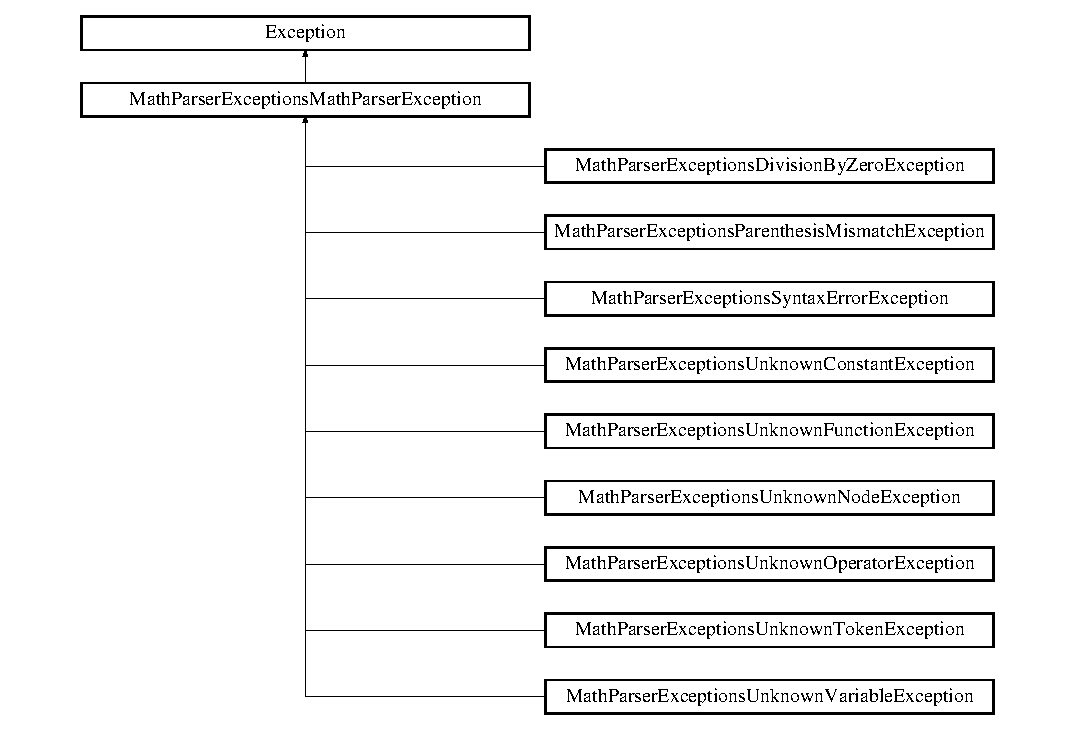
\includegraphics[height=9.361702cm]{classMathParser_1_1Exceptions_1_1MathParserException}
\end{center}
\end{figure}


The documentation for this class was generated from the following file\-:\begin{DoxyCompactItemize}
\item 
src/\-Math\-Parser/\-Exceptions/Math\-Parser\-Exception.\-php\end{DoxyCompactItemize}

\hypertarget{classMathParser_1_1Parsing_1_1Nodes_1_1Node}{\section{Math\-Parser\textbackslash{}Parsing\textbackslash{}Nodes\textbackslash{}Node Class Reference}
\label{classMathParser_1_1Parsing_1_1Nodes_1_1Node}\index{Math\-Parser\textbackslash{}\-Parsing\textbackslash{}\-Nodes\textbackslash{}\-Node@{Math\-Parser\textbackslash{}\-Parsing\textbackslash{}\-Nodes\textbackslash{}\-Node}}
}
Inheritance diagram for Math\-Parser\textbackslash{}Parsing\textbackslash{}Nodes\textbackslash{}Node\-:\begin{figure}[H]
\begin{center}
\leavevmode
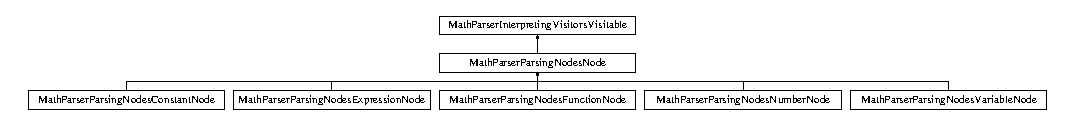
\includegraphics[height=1.249071cm]{classMathParser_1_1Parsing_1_1Nodes_1_1Node}
\end{center}
\end{figure}
\subsection*{Public Member Functions}
\begin{DoxyCompactItemize}
\item 
\hyperlink{classMathParser_1_1Parsing_1_1Nodes_1_1Node_aa365c3dd42885fc67f00f88578994788}{evaluate} (\$variables)
\begin{DoxyCompactList}\small\item\em Convenience function for evaluating a tree, using the Evaluator class. \end{DoxyCompactList}\item 
\hypertarget{classMathParser_1_1Parsing_1_1Nodes_1_1Node_a607d20250ecf48ac6842531cde46daff}{{\bfseries complexity} ()}\label{classMathParser_1_1Parsing_1_1Nodes_1_1Node_a607d20250ecf48ac6842531cde46daff}

\end{DoxyCompactItemize}
\subsection*{Static Public Member Functions}
\begin{DoxyCompactItemize}
\item 
\hypertarget{classMathParser_1_1Parsing_1_1Nodes_1_1Node_ad6545a234a585ce6dad63c6337483cb7}{static {\bfseries factory} (\hyperlink{classMathParser_1_1Lexing_1_1Token}{Token} \$token)}\label{classMathParser_1_1Parsing_1_1Nodes_1_1Node_ad6545a234a585ce6dad63c6337483cb7}

\item 
\hypertarget{classMathParser_1_1Parsing_1_1Nodes_1_1Node_a9d672f21f7fa25a3cfe0a940d3643b97}{static {\bfseries compare\-Nodes} (\$node1, \$node2)}\label{classMathParser_1_1Parsing_1_1Nodes_1_1Node_a9d672f21f7fa25a3cfe0a940d3643b97}

\end{DoxyCompactItemize}


\subsection{Member Function Documentation}
\hypertarget{classMathParser_1_1Parsing_1_1Nodes_1_1Node_aa365c3dd42885fc67f00f88578994788}{\index{Math\-Parser\-::\-Parsing\-::\-Nodes\-::\-Node@{Math\-Parser\-::\-Parsing\-::\-Nodes\-::\-Node}!evaluate@{evaluate}}
\index{evaluate@{evaluate}!MathParser::Parsing::Nodes::Node@{Math\-Parser\-::\-Parsing\-::\-Nodes\-::\-Node}}
\subsubsection[{evaluate}]{\setlength{\rightskip}{0pt plus 5cm}Math\-Parser\textbackslash{}\-Parsing\textbackslash{}\-Nodes\textbackslash{}\-Node\-::evaluate (
\begin{DoxyParamCaption}
\item[{}]{\$variables}
\end{DoxyParamCaption}
)}}\label{classMathParser_1_1Parsing_1_1Nodes_1_1Node_aa365c3dd42885fc67f00f88578994788}


Convenience function for evaluating a tree, using the Evaluator class. 

Example usage\-: \$parser = new Std\-Math\-Parser(); \$node = \$parser-\/$>$parse('sin(x)cos(y)'); \$function\-Value = \$node-\/$>$evaluate( array( 'x' =$>$ 1.\-3, 'y' =$>$ 1.\-4 ) );


\begin{DoxyParams}[1]{Parameters}
array & {\em \$variables} & key-\/value array of variable values \\
\hline
\end{DoxyParams}

\begin{DoxyRetVals}{Return values}
{\em floatval} & \\
\hline
\end{DoxyRetVals}


The documentation for this class was generated from the following file\-:\begin{DoxyCompactItemize}
\item 
src/\-Math\-Parser/\-Parsing/\-Nodes/Node.\-php\end{DoxyCompactItemize}

\hypertarget{classMathParser_1_1Parsing_1_1Nodes_1_1NumberNode}{\section{Math\-Parser\textbackslash{}Parsing\textbackslash{}Nodes\textbackslash{}Number\-Node Class Reference}
\label{classMathParser_1_1Parsing_1_1Nodes_1_1NumberNode}\index{Math\-Parser\textbackslash{}\-Parsing\textbackslash{}\-Nodes\textbackslash{}\-Number\-Node@{Math\-Parser\textbackslash{}\-Parsing\textbackslash{}\-Nodes\textbackslash{}\-Number\-Node}}
}


A\-S\-T node representing a number (int or float)  


Inheritance diagram for Math\-Parser\textbackslash{}Parsing\textbackslash{}Nodes\textbackslash{}Number\-Node\-:\begin{figure}[H]
\begin{center}
\leavevmode
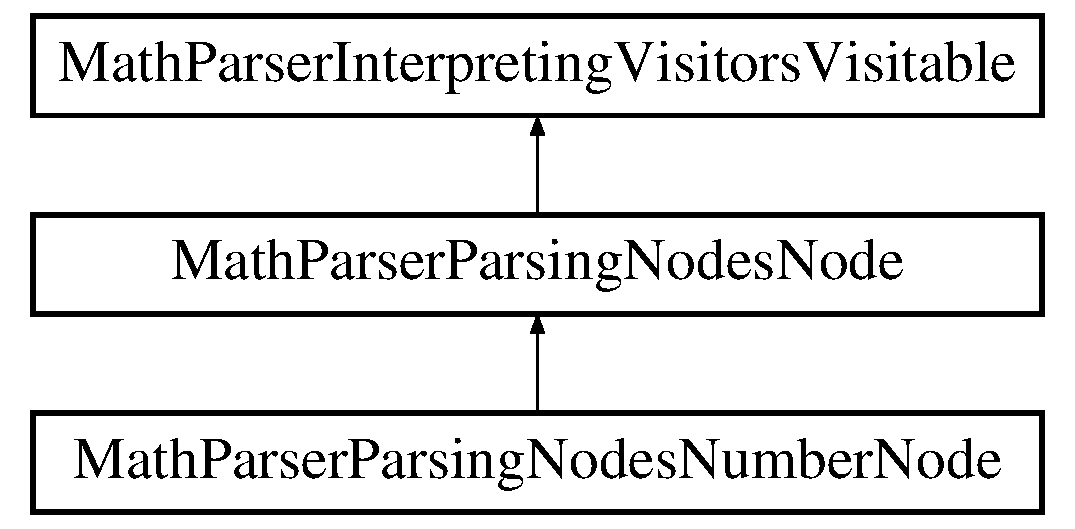
\includegraphics[height=3.000000cm]{classMathParser_1_1Parsing_1_1Nodes_1_1NumberNode}
\end{center}
\end{figure}
\subsection*{Public Member Functions}
\begin{DoxyCompactItemize}
\item 
\hypertarget{classMathParser_1_1Parsing_1_1Nodes_1_1NumberNode_abf2cc9dcf5655fcd73d6045a39008835}{{\bfseries \-\_\-\-\_\-construct} (\$value)}\label{classMathParser_1_1Parsing_1_1Nodes_1_1NumberNode_abf2cc9dcf5655fcd73d6045a39008835}

\item 
\hyperlink{classMathParser_1_1Parsing_1_1Nodes_1_1NumberNode_a9929ffd441d3753c1244be6667cd13fb}{get\-Value} ()
\begin{DoxyCompactList}\small\item\em Returns the value. \end{DoxyCompactList}\item 
\hypertarget{classMathParser_1_1Parsing_1_1Nodes_1_1NumberNode_afe0acdb60d40d8f053a00cddef53a2d4}{\hyperlink{classMathParser_1_1Parsing_1_1Nodes_1_1NumberNode_afe0acdb60d40d8f053a00cddef53a2d4}{accept} (\hyperlink{interfaceMathParser_1_1Interpreting_1_1Visitors_1_1Visitor}{Visitor} \$visitor)}\label{classMathParser_1_1Parsing_1_1Nodes_1_1NumberNode_afe0acdb60d40d8f053a00cddef53a2d4}

\begin{DoxyCompactList}\small\item\em Implementing the Visitable interface. \end{DoxyCompactList}\end{DoxyCompactItemize}
\subsection*{Private Attributes}
\begin{DoxyCompactItemize}
\item 
\hypertarget{classMathParser_1_1Parsing_1_1Nodes_1_1NumberNode_a8aa753c37f3b8800bb0fba8087659849}{{\bfseries \$value}}\label{classMathParser_1_1Parsing_1_1Nodes_1_1NumberNode_a8aa753c37f3b8800bb0fba8087659849}

\end{DoxyCompactItemize}
\subsection*{Additional Inherited Members}


\subsection{Detailed Description}
A\-S\-T node representing a number (int or float) 

\subsection{Member Function Documentation}
\hypertarget{classMathParser_1_1Parsing_1_1Nodes_1_1NumberNode_a9929ffd441d3753c1244be6667cd13fb}{\index{Math\-Parser\-::\-Parsing\-::\-Nodes\-::\-Number\-Node@{Math\-Parser\-::\-Parsing\-::\-Nodes\-::\-Number\-Node}!get\-Value@{get\-Value}}
\index{get\-Value@{get\-Value}!MathParser::Parsing::Nodes::NumberNode@{Math\-Parser\-::\-Parsing\-::\-Nodes\-::\-Number\-Node}}
\subsubsection[{get\-Value}]{\setlength{\rightskip}{0pt plus 5cm}Math\-Parser\textbackslash{}\-Parsing\textbackslash{}\-Nodes\textbackslash{}\-Number\-Node\-::get\-Value (
\begin{DoxyParamCaption}
{}
\end{DoxyParamCaption}
)}}\label{classMathParser_1_1Parsing_1_1Nodes_1_1NumberNode_a9929ffd441d3753c1244be6667cd13fb}


Returns the value. 


\begin{DoxyRetVals}{Return values}
{\em int$\vert$float} & \\
\hline
\end{DoxyRetVals}


The documentation for this class was generated from the following file\-:\begin{DoxyCompactItemize}
\item 
src/\-Math\-Parser/\-Parsing/\-Nodes/Number\-Node.\-php\end{DoxyCompactItemize}

\hypertarget{classMathParser_1_1Exceptions_1_1ParenthesisMismatchException}{\section{Math\-Parser\textbackslash{}Exceptions\textbackslash{}Parenthesis\-Mismatch\-Exception Class Reference}
\label{classMathParser_1_1Exceptions_1_1ParenthesisMismatchException}\index{Math\-Parser\textbackslash{}\-Exceptions\textbackslash{}\-Parenthesis\-Mismatch\-Exception@{Math\-Parser\textbackslash{}\-Exceptions\textbackslash{}\-Parenthesis\-Mismatch\-Exception}}
}
Inheritance diagram for Math\-Parser\textbackslash{}Exceptions\textbackslash{}Parenthesis\-Mismatch\-Exception\-:\begin{figure}[H]
\begin{center}
\leavevmode
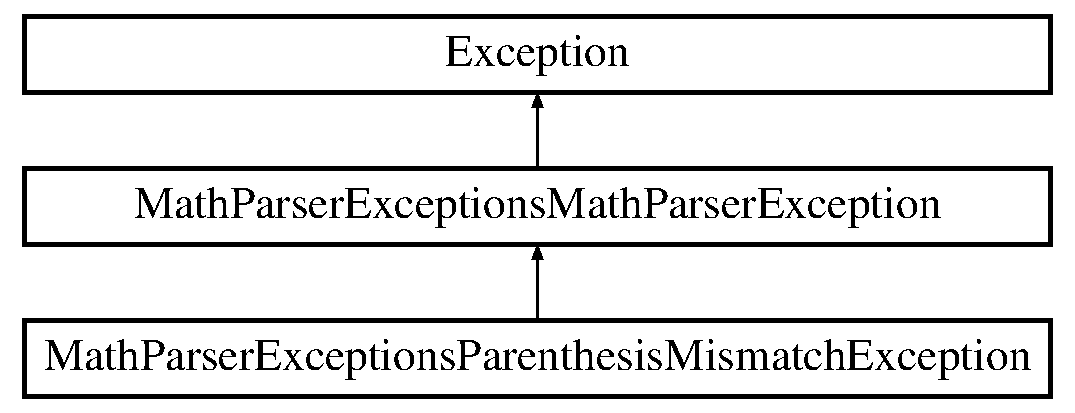
\includegraphics[height=3.000000cm]{classMathParser_1_1Exceptions_1_1ParenthesisMismatchException}
\end{center}
\end{figure}


The documentation for this class was generated from the following file\-:\begin{DoxyCompactItemize}
\item 
src/\-Math\-Parser/\-Exceptions/Parenthesis\-Mismatch\-Exception.\-php\end{DoxyCompactItemize}

\hypertarget{classMathParser_1_1Parsing_1_1Parser}{\section{Math\-Parser\textbackslash{}Parsing\textbackslash{}Parser Class Reference}
\label{classMathParser_1_1Parsing_1_1Parser}\index{Math\-Parser\textbackslash{}\-Parsing\textbackslash{}\-Parser@{Math\-Parser\textbackslash{}\-Parsing\textbackslash{}\-Parser}}
}


Mathematical expression parser, based on the shunting yard algorithm.  


\subsection*{Public Member Functions}
\begin{DoxyCompactItemize}
\item 
\hyperlink{classMathParser_1_1Parsing_1_1Parser_a556c64ee108e141b442badafbd3b1164}{parse} (array \$tokens)
\begin{DoxyCompactList}\small\item\em Parse list of tokens. \end{DoxyCompactList}\end{DoxyCompactItemize}
\subsection*{Protected Member Functions}
\begin{DoxyCompactItemize}
\item 
\hyperlink{classMathParser_1_1Parsing_1_1Parser_a2572d3c71a4fd638bb0e9188c2e7f7e9}{handle\-Expression} (\$token)
\begin{DoxyCompactList}\small\item\em Create an appropriate Node from the corresponding token. \end{DoxyCompactList}\item 
\hyperlink{classMathParser_1_1Parsing_1_1Parser_a0896b00bcb6831560faea77f5ff7831c}{filter\-Tokens} (array \$tokens)
\begin{DoxyCompactList}\small\item\em Remove Whitespace from the token list. \end{DoxyCompactList}\item 
\hyperlink{classMathParser_1_1Parsing_1_1Parser_a74e79e5a38c1edbc919cd66c50712cd8}{parse\-Implicit\-Multiplication} (array \$tokens)
\begin{DoxyCompactList}\small\item\em Insert multiplication tokens where needed (taking care of implicit mulitplication). \end{DoxyCompactList}\end{DoxyCompactItemize}
\subsection*{Static Protected Member Functions}
\begin{DoxyCompactItemize}
\item 
static \hyperlink{classMathParser_1_1Parsing_1_1Parser_ab559cd696a23ad1eeddb69eb6a56a067}{allow\-Implicit\-Multiplication} ()
\begin{DoxyCompactList}\small\item\em Determine if the parser allows implicit multiplication. \end{DoxyCompactList}\end{DoxyCompactItemize}
\subsection*{Protected Attributes}
\begin{DoxyCompactItemize}
\item 
\hypertarget{classMathParser_1_1Parsing_1_1Parser_ab20fd2f0971594016b8b631d29532284}{{\bfseries \$tokens}}\label{classMathParser_1_1Parsing_1_1Parser_ab20fd2f0971594016b8b631d29532284}

\item 
\hypertarget{classMathParser_1_1Parsing_1_1Parser_a6a691e6b115de82b04fa5b2fc828721b}{{\bfseries \$operator\-Stack}}\label{classMathParser_1_1Parsing_1_1Parser_a6a691e6b115de82b04fa5b2fc828721b}

\item 
\hypertarget{classMathParser_1_1Parsing_1_1Parser_a761f3ca46141d5e39e620520a2a876fa}{{\bfseries \$operand\-Stack}}\label{classMathParser_1_1Parsing_1_1Parser_a761f3ca46141d5e39e620520a2a876fa}

\end{DoxyCompactItemize}
\subsection*{Private Member Functions}
\begin{DoxyCompactItemize}
\item 
\hyperlink{classMathParser_1_1Parsing_1_1Parser_a5e95881d4b53730565bf2205fa621086}{Shunting\-Yard} (array \$tokens)
\begin{DoxyCompactList}\small\item\em Implementation of the shunting yard parsing algorithm. \end{DoxyCompactList}\end{DoxyCompactItemize}


\subsection{Detailed Description}
Mathematical expression parser, based on the shunting yard algorithm. 

Parse a token string into an abstract syntax tree (A\-S\-T).

As the parser loops over the individual tokens, two stacks are kept up to date. One stack (\$operator\-Stack) consists of hitherto unhandled tokens corresponding to ''operators'' (unary and binary operators, function applications and parenthesis) and a stack of parsed sub-\/expressions (the \$operand\-Stack).

If the current token is a terminal token (number, variable or constant), a corresponding node is pushed onto the operand\-Stack.

Otherwise, the precedence of the current token is compared to the top element(t) on the operator\-Stack, and as long as the current token has lower precedence, we keep popping operators from the stack to constuct more complicated subexpressions together with the top items on the operand\-Stack.

Once the token list is empty, we pop the remaining operators as above, and if the formula was well-\/formed, the only thing remaining on the operand\-Stack is a completely parsed A\-S\-T, which we return. 

\subsection{Member Function Documentation}
\hypertarget{classMathParser_1_1Parsing_1_1Parser_ab559cd696a23ad1eeddb69eb6a56a067}{\index{Math\-Parser\-::\-Parsing\-::\-Parser@{Math\-Parser\-::\-Parsing\-::\-Parser}!allow\-Implicit\-Multiplication@{allow\-Implicit\-Multiplication}}
\index{allow\-Implicit\-Multiplication@{allow\-Implicit\-Multiplication}!MathParser::Parsing::Parser@{Math\-Parser\-::\-Parsing\-::\-Parser}}
\subsubsection[{allow\-Implicit\-Multiplication}]{\setlength{\rightskip}{0pt plus 5cm}Math\-Parser\textbackslash{}\-Parsing\textbackslash{}\-Parser\-::allow\-Implicit\-Multiplication (
\begin{DoxyParamCaption}
{}
\end{DoxyParamCaption}
)\hspace{0.3cm}{\ttfamily [static]}, {\ttfamily [protected]}}}\label{classMathParser_1_1Parsing_1_1Parser_ab559cd696a23ad1eeddb69eb6a56a067}


Determine if the parser allows implicit multiplication. 

Create a subclass of \hyperlink{classMathParser_1_1Parsing_1_1Parser}{Parser}, overriding this function, returning false instead to diallow implicit multiplication.

\paragraph*{Example\-:}


\begin{DoxyCode}
\textcolor{keyword}{class }ParserWithoutImplictMultiplication \textcolor{keyword}{extends} Parser \{
  \textcolor{keyword}{protected} \textcolor{keyword}{function} \hyperlink{classMathParser_1_1Parsing_1_1Parser_ab559cd696a23ad1eeddb69eb6a56a067}{allowImplicitMultiplication}() \{
    \textcolor{keywordflow}{return} \textcolor{keyword}{false};
  \}
\}

$lexer = \textcolor{keyword}{new} StdMathLexer();
$tokens = $lexer->tokenize(\textcolor{stringliteral}{'2x'});
$parser = \textcolor{keyword}{new} ParserWithoutImplicitMultiplication();
$node = $parser->parse($tokens); \textcolor{comment}{// Throws a SyntaxErrorException}
\end{DoxyCode}



\begin{DoxyRetVals}{Return values}
{\em boolean} & \\
\hline
\end{DoxyRetVals}
\hypertarget{classMathParser_1_1Parsing_1_1Parser_a0896b00bcb6831560faea77f5ff7831c}{\index{Math\-Parser\-::\-Parsing\-::\-Parser@{Math\-Parser\-::\-Parsing\-::\-Parser}!filter\-Tokens@{filter\-Tokens}}
\index{filter\-Tokens@{filter\-Tokens}!MathParser::Parsing::Parser@{Math\-Parser\-::\-Parsing\-::\-Parser}}
\subsubsection[{filter\-Tokens}]{\setlength{\rightskip}{0pt plus 5cm}Math\-Parser\textbackslash{}\-Parsing\textbackslash{}\-Parser\-::filter\-Tokens (
\begin{DoxyParamCaption}
\item[{array}]{\$tokens}
\end{DoxyParamCaption}
)\hspace{0.3cm}{\ttfamily [protected]}}}\label{classMathParser_1_1Parsing_1_1Parser_a0896b00bcb6831560faea77f5ff7831c}


Remove Whitespace from the token list. 


\begin{DoxyParams}{Parameters}
{\em Token\mbox{[}$\,$\mbox{]}} & \$tokens Input list of tokens \\
\hline
\end{DoxyParams}

\begin{DoxyRetVals}{Return values}
{\em Token\mbox{[}$\,$\mbox{]}} & \\
\hline
\end{DoxyRetVals}
\hypertarget{classMathParser_1_1Parsing_1_1Parser_a2572d3c71a4fd638bb0e9188c2e7f7e9}{\index{Math\-Parser\-::\-Parsing\-::\-Parser@{Math\-Parser\-::\-Parsing\-::\-Parser}!handle\-Expression@{handle\-Expression}}
\index{handle\-Expression@{handle\-Expression}!MathParser::Parsing::Parser@{Math\-Parser\-::\-Parsing\-::\-Parser}}
\subsubsection[{handle\-Expression}]{\setlength{\rightskip}{0pt plus 5cm}Math\-Parser\textbackslash{}\-Parsing\textbackslash{}\-Parser\-::handle\-Expression (
\begin{DoxyParamCaption}
\item[{}]{\$token}
\end{DoxyParamCaption}
)\hspace{0.3cm}{\ttfamily [protected]}}}\label{classMathParser_1_1Parsing_1_1Parser_a2572d3c71a4fd638bb0e9188c2e7f7e9}


Create an appropriate Node from the corresponding token. 


\begin{DoxyParams}[1]{Parameters}
Token & {\em \$token} & \\
\hline
\end{DoxyParams}

\begin{DoxyRetVals}{Return values}
{\em Node} & \\
\hline
\end{DoxyRetVals}

\begin{DoxyExceptions}{Exceptions}
{\em Syntax\-Error\-Exception} & \\
\hline
\end{DoxyExceptions}
\hypertarget{classMathParser_1_1Parsing_1_1Parser_a556c64ee108e141b442badafbd3b1164}{\index{Math\-Parser\-::\-Parsing\-::\-Parser@{Math\-Parser\-::\-Parsing\-::\-Parser}!parse@{parse}}
\index{parse@{parse}!MathParser::Parsing::Parser@{Math\-Parser\-::\-Parsing\-::\-Parser}}
\subsubsection[{parse}]{\setlength{\rightskip}{0pt plus 5cm}Math\-Parser\textbackslash{}\-Parsing\textbackslash{}\-Parser\-::parse (
\begin{DoxyParamCaption}
\item[{array}]{\$tokens}
\end{DoxyParamCaption}
)}}\label{classMathParser_1_1Parsing_1_1Parser_a556c64ee108e141b442badafbd3b1164}


Parse list of tokens. 


\begin{DoxyParams}{Parameters}
{\em Token\mbox{[}$\,$\mbox{]}} & \$tokens \\
\hline
\end{DoxyParams}

\begin{DoxyRetVals}{Return values}
{\em Node} & \\
\hline
\end{DoxyRetVals}
\hypertarget{classMathParser_1_1Parsing_1_1Parser_a74e79e5a38c1edbc919cd66c50712cd8}{\index{Math\-Parser\-::\-Parsing\-::\-Parser@{Math\-Parser\-::\-Parsing\-::\-Parser}!parse\-Implicit\-Multiplication@{parse\-Implicit\-Multiplication}}
\index{parse\-Implicit\-Multiplication@{parse\-Implicit\-Multiplication}!MathParser::Parsing::Parser@{Math\-Parser\-::\-Parsing\-::\-Parser}}
\subsubsection[{parse\-Implicit\-Multiplication}]{\setlength{\rightskip}{0pt plus 5cm}Math\-Parser\textbackslash{}\-Parsing\textbackslash{}\-Parser\-::parse\-Implicit\-Multiplication (
\begin{DoxyParamCaption}
\item[{array}]{\$tokens}
\end{DoxyParamCaption}
)\hspace{0.3cm}{\ttfamily [protected]}}}\label{classMathParser_1_1Parsing_1_1Parser_a74e79e5a38c1edbc919cd66c50712cd8}


Insert multiplication tokens where needed (taking care of implicit mulitplication). 


\begin{DoxyParams}{Parameters}
{\em Token\mbox{[}$\,$\mbox{]}} & \$tokens Input list of tokens \\
\hline
\end{DoxyParams}

\begin{DoxyRetVals}{Return values}
{\em Token\mbox{[}$\,$\mbox{]}} & \\
\hline
\end{DoxyRetVals}
\hypertarget{classMathParser_1_1Parsing_1_1Parser_a5e95881d4b53730565bf2205fa621086}{\index{Math\-Parser\-::\-Parsing\-::\-Parser@{Math\-Parser\-::\-Parsing\-::\-Parser}!Shunting\-Yard@{Shunting\-Yard}}
\index{Shunting\-Yard@{Shunting\-Yard}!MathParser::Parsing::Parser@{Math\-Parser\-::\-Parsing\-::\-Parser}}
\subsubsection[{Shunting\-Yard}]{\setlength{\rightskip}{0pt plus 5cm}Math\-Parser\textbackslash{}\-Parsing\textbackslash{}\-Parser\-::\-Shunting\-Yard (
\begin{DoxyParamCaption}
\item[{array}]{\$tokens}
\end{DoxyParamCaption}
)\hspace{0.3cm}{\ttfamily [private]}}}\label{classMathParser_1_1Parsing_1_1Parser_a5e95881d4b53730565bf2205fa621086}


Implementation of the shunting yard parsing algorithm. 


\begin{DoxyParams}{Parameters}
{\em Token\mbox{[}$\,$\mbox{]}} & \$tokens \\
\hline
\end{DoxyParams}

\begin{DoxyRetVals}{Return values}
{\em Node} & \\
\hline
\end{DoxyRetVals}

\begin{DoxyExceptions}{Exceptions}
{\em Syntax\-Error\-Exception} & \\
\hline
{\em Parenthesis\-Mismatch\-Exception} & \\
\hline
\end{DoxyExceptions}


The documentation for this class was generated from the following file\-:\begin{DoxyCompactItemize}
\item 
src/\-Math\-Parser/\-Parsing/Parser.\-php\end{DoxyCompactItemize}

\hypertarget{classMathParser_1_1Parsing_1_1Stack}{\section{Math\-Parser\textbackslash{}Parsing\textbackslash{}Stack Class Reference}
\label{classMathParser_1_1Parsing_1_1Stack}\index{Math\-Parser\textbackslash{}\-Parsing\textbackslash{}\-Stack@{Math\-Parser\textbackslash{}\-Parsing\textbackslash{}\-Stack}}
}
\subsection*{Public Member Functions}
\begin{DoxyCompactItemize}
\item 
\hypertarget{classMathParser_1_1Parsing_1_1Stack_a50f3a135fdf9401b17494c50652b152a}{{\bfseries push} (\$element)}\label{classMathParser_1_1Parsing_1_1Stack_a50f3a135fdf9401b17494c50652b152a}

\item 
\hypertarget{classMathParser_1_1Parsing_1_1Stack_a13b5dc80388b7900af165e0822ebec93}{{\bfseries peek} ()}\label{classMathParser_1_1Parsing_1_1Stack_a13b5dc80388b7900af165e0822ebec93}

\item 
\hypertarget{classMathParser_1_1Parsing_1_1Stack_a23eff250a1077d7a9838a88e6755a84a}{{\bfseries pop} ()}\label{classMathParser_1_1Parsing_1_1Stack_a23eff250a1077d7a9838a88e6755a84a}

\item 
\hypertarget{classMathParser_1_1Parsing_1_1Stack_ad85713b07820a24a6e781b32e18271e6}{{\bfseries count} ()}\label{classMathParser_1_1Parsing_1_1Stack_ad85713b07820a24a6e781b32e18271e6}

\end{DoxyCompactItemize}
\subsection*{Public Attributes}
\begin{DoxyCompactItemize}
\item 
\hypertarget{classMathParser_1_1Parsing_1_1Stack_ab508efbeda55b29432f6aefbb591ca10}{{\bfseries \$data} = array()}\label{classMathParser_1_1Parsing_1_1Stack_ab508efbeda55b29432f6aefbb591ca10}

\end{DoxyCompactItemize}


The documentation for this class was generated from the following file\-:\begin{DoxyCompactItemize}
\item 
src/\-Math\-Parser/\-Parsing/Stack.\-php\end{DoxyCompactItemize}

\hypertarget{classMathParser_1_1Lexing_1_1StdMathLexer}{\section{Math\-Parser\textbackslash{}Lexing\textbackslash{}Std\-Math\-Lexer Class Reference}
\label{classMathParser_1_1Lexing_1_1StdMathLexer}\index{Math\-Parser\textbackslash{}\-Lexing\textbackslash{}\-Std\-Math\-Lexer@{Math\-Parser\textbackslash{}\-Lexing\textbackslash{}\-Std\-Math\-Lexer}}
}


\hyperlink{classMathParser_1_1Lexing_1_1Lexer}{Lexer} capable of recognizing all standard mathematical expressions.  


Inheritance diagram for Math\-Parser\textbackslash{}Lexing\textbackslash{}Std\-Math\-Lexer\-:\begin{figure}[H]
\begin{center}
\leavevmode
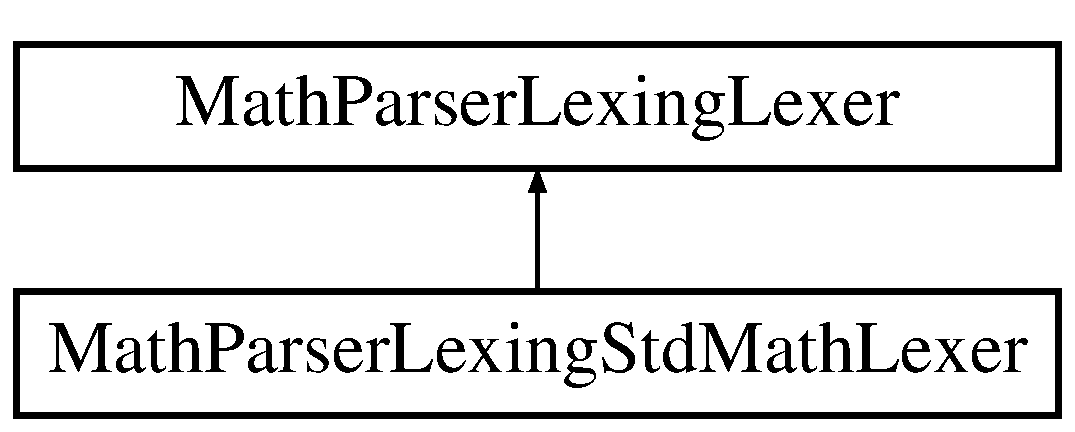
\includegraphics[height=2.000000cm]{classMathParser_1_1Lexing_1_1StdMathLexer}
\end{center}
\end{figure}
\subsection*{Additional Inherited Members}


\subsection{Detailed Description}
\hyperlink{classMathParser_1_1Lexing_1_1Lexer}{Lexer} capable of recognizing all standard mathematical expressions. 

Subclass of the generic \hyperlink{classMathParser_1_1Lexing_1_1Lexer}{Lexer}, with \hyperlink{classMathParser_1_1Lexing_1_1TokenDefinition}{Token\-Definition} patterns for numbers, elementary functions, arithmetic operations and variables.

\paragraph*{Recognized tokens}


\begin{DoxyItemize}
\item {\ttfamily /?\textbackslash{}d+/} matching integers matching
\item {\ttfamily /sqrt/} matching square root function
\item {\ttfamily /sinh/} matching hyperbolic sine
\item {\ttfamily /cosh/} matching hyperbolic cosine
\item {\ttfamily /tanh/} matching hyperbolic tangent
\item {\ttfamily /coth/} matching hyperbolic cotangent
\item {\ttfamily /sin/} matching sine
\item {\ttfamily /cos/} matching cosine
\item {\ttfamily /tan/} matching tangent
\item {\ttfamily /cot/} matching cotangent
\item {\ttfamily /arsinh$\vert$arcsinh$\vert$asinh/} matching inverse hyperbolic sine
\item {\ttfamily /arcosh$\vert$arccosh$\vert$acosh/} matching inverse hyperbolic cosine
\item {\ttfamily /artanh$\vert$arctanh$\vert$atanh/} matching inverse hyperbolic tangent
\item {\ttfamily /arcoth$\vert$arccoth$\vert$acoth/} matching inverse hyperbolic cotangent
\item {\ttfamily /arcsin$\vert$asin/} matching inverse sine
\item {\ttfamily /arccos$\vert$acos/} matching inverse cosine
\item {\ttfamily /arctan$\vert$atan/} matching inverse tangent
\item {\ttfamily /arccot$\vert$acot/} matching inverse cotangent
\item {\ttfamily /exp/} matching exponential function
\item {\ttfamily /log10$\vert$lg/} matching logarithm (base 10)
\item {\ttfamily /log$\vert$ln/} matching natural logarithm
\item {\ttfamily /\textbackslash{}(/} matching opening parenthesis (both as delimiter and function evaluation)
\item {\ttfamily /\textbackslash{})/} matching closing parenthesisis (both as delimiter and function evaluation)
\item {\ttfamily /\textbackslash{}+/} matching + for addition (or unary +)
\item {\ttfamily /\textbackslash{}-\//} matching -\/ for subtraction (or unary -\/)
\item {\ttfamily /\textbackslash{}$\ast$ /} matching $\ast$ for multiplication
\item {\ttfamily /\textbackslash{}//} matching / for division
\item {\ttfamily /\textbackslash{}$^\wedge$/} matching $^\wedge$ for exponentiation
\item {\ttfamily /pi/} matching constant pi
\item {\ttfamily /e/} matching constant e
\item {\ttfamily /\mbox{[}a-\/z\-A-\/\-Z\mbox{]}/} matching variables (note that we only allow single letter identifiers, this improves parsing of implicit multiplication)
\item {\ttfamily /\textbackslash{}n/} matching newline
\item {\ttfamily /\textbackslash{}s+/} matching whitespace 
\end{DoxyItemize}

The documentation for this class was generated from the following file\-:\begin{DoxyCompactItemize}
\item 
src/\-Math\-Parser/\-Lexing/Std\-Math\-Lexer.\-php\end{DoxyCompactItemize}

\hypertarget{classMathParser_1_1StdMathParser}{\section{Math\-Parser\textbackslash{}Std\-Math\-Parser Class Reference}
\label{classMathParser_1_1StdMathParser}\index{Math\-Parser\textbackslash{}\-Std\-Math\-Parser@{Math\-Parser\textbackslash{}\-Std\-Math\-Parser}}
}
\subsection*{Public Member Functions}
\begin{DoxyCompactItemize}
\item 
\hypertarget{classMathParser_1_1StdMathParser_a582d6ace9e6ef10d6d3314d82496c5cc}{{\bfseries \-\_\-\-\_\-construct} (\$debug=false)}\label{classMathParser_1_1StdMathParser_a582d6ace9e6ef10d6d3314d82496c5cc}

\item 
\hypertarget{classMathParser_1_1StdMathParser_a8eb08ff6c902fc7c1d01cf5ec14c67a5}{{\bfseries parse} (\$text)}\label{classMathParser_1_1StdMathParser_a8eb08ff6c902fc7c1d01cf5ec14c67a5}

\item 
\hypertarget{classMathParser_1_1StdMathParser_a656006e54a870b98dfa9352e7cc02ebe}{{\bfseries get\-Token\-List} ()}\label{classMathParser_1_1StdMathParser_a656006e54a870b98dfa9352e7cc02ebe}

\item 
\hypertarget{classMathParser_1_1StdMathParser_a9c824c8b42c4ed45b4b6b212eb06b617}{{\bfseries get\-Tree} ()}\label{classMathParser_1_1StdMathParser_a9c824c8b42c4ed45b4b6b212eb06b617}

\end{DoxyCompactItemize}
\subsection*{Private Attributes}
\begin{DoxyCompactItemize}
\item 
\hypertarget{classMathParser_1_1StdMathParser_ab6946ba25d66a75b424eae04d5cb070d}{{\bfseries \$lexer}}\label{classMathParser_1_1StdMathParser_ab6946ba25d66a75b424eae04d5cb070d}

\item 
\hypertarget{classMathParser_1_1StdMathParser_abd2f22d467ff3c59cf47907209baa6cd}{{\bfseries \$parser}}\label{classMathParser_1_1StdMathParser_abd2f22d467ff3c59cf47907209baa6cd}

\item 
\hypertarget{classMathParser_1_1StdMathParser_a7df1405869c2a0fdc4cbe8a47fe24b79}{{\bfseries \$tokens}}\label{classMathParser_1_1StdMathParser_a7df1405869c2a0fdc4cbe8a47fe24b79}

\item 
\hypertarget{classMathParser_1_1StdMathParser_a520e08ff2d81d78f211e11ed7d9b8a23}{{\bfseries \$tree}}\label{classMathParser_1_1StdMathParser_a520e08ff2d81d78f211e11ed7d9b8a23}

\end{DoxyCompactItemize}


The documentation for this class was generated from the following file\-:\begin{DoxyCompactItemize}
\item 
src/\-Math\-Parser/Std\-Math\-Parser.\-php\end{DoxyCompactItemize}

\hypertarget{classMathParser_1_1Exceptions_1_1SyntaxErrorException}{\section{Math\-Parser\textbackslash{}Exceptions\textbackslash{}Syntax\-Error\-Exception Class Reference}
\label{classMathParser_1_1Exceptions_1_1SyntaxErrorException}\index{Math\-Parser\textbackslash{}\-Exceptions\textbackslash{}\-Syntax\-Error\-Exception@{Math\-Parser\textbackslash{}\-Exceptions\textbackslash{}\-Syntax\-Error\-Exception}}
}
Inheritance diagram for Math\-Parser\textbackslash{}Exceptions\textbackslash{}Syntax\-Error\-Exception\-:\begin{figure}[H]
\begin{center}
\leavevmode
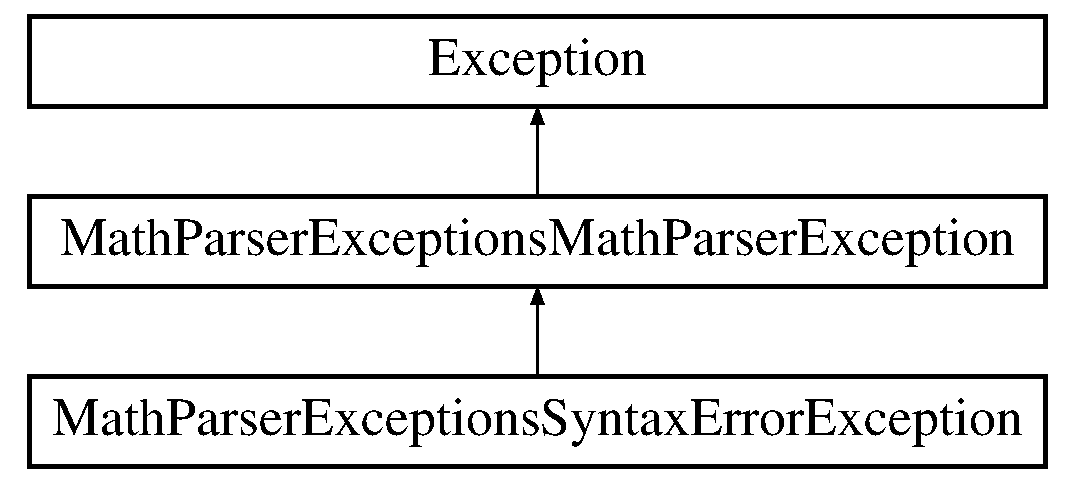
\includegraphics[height=2.000000cm]{classMathParser_1_1Exceptions_1_1SyntaxErrorException}
\end{center}
\end{figure}


The documentation for this class was generated from the following file\-:\begin{DoxyCompactItemize}
\item 
src/\-Math\-Parser/\-Exceptions/Syntax\-Error\-Exception.\-php\end{DoxyCompactItemize}

\hypertarget{classMathParser_1_1Lexing_1_1Token}{\section{Math\-Parser\textbackslash{}Lexing\textbackslash{}Token Class Reference}
\label{classMathParser_1_1Lexing_1_1Token}\index{Math\-Parser\textbackslash{}\-Lexing\textbackslash{}\-Token@{Math\-Parser\textbackslash{}\-Lexing\textbackslash{}\-Token}}
}


\hyperlink{classMathParser_1_1Lexing_1_1Token}{Token} class.  


\subsection*{Public Member Functions}
\begin{DoxyCompactItemize}
\item 
\hyperlink{classMathParser_1_1Lexing_1_1Token_a45ded5abf4fef1a2e8938f71d8864491}{\-\_\-\-\_\-construct} (\$value, \$type, \$match=null)
\begin{DoxyCompactList}\small\item\em Public constructor. \end{DoxyCompactList}\item 
\hyperlink{classMathParser_1_1Lexing_1_1Token_abdd998ce6d440c0773fa7fa3616cf79b}{length} ()
\begin{DoxyCompactList}\small\item\em Length of the input string matching the token. \end{DoxyCompactList}\item 
\hyperlink{classMathParser_1_1Lexing_1_1Token_a1dac568b5f1008243edcf1b00d13cf42}{get\-Value} ()
\begin{DoxyCompactList}\small\item\em Standarized value/name of the \hyperlink{classMathParser_1_1Lexing_1_1Token}{Token}, usually the same as what was matched in the the input string. \end{DoxyCompactList}\item 
\hyperlink{classMathParser_1_1Lexing_1_1Token_a695571048ecc4c9bab3c742a676fac67}{get\-Type} ()
\begin{DoxyCompactList}\small\item\em Returns the type of the token, as defined in the \hyperlink{classMathParser_1_1Lexing_1_1TokenType}{Token\-Type} class. \end{DoxyCompactList}\item 
\hyperlink{classMathParser_1_1Lexing_1_1Token_abbb8a5b874586940b6023c53233149b0}{get\-Precedence} ()
\begin{DoxyCompactList}\small\item\em Returns the precedence/priority of the token, as defined by the \hyperlink{classMathParser_1_1Lexing_1_1TokenPrecedence}{Token\-Precedence} class. \end{DoxyCompactList}\item 
\hyperlink{classMathParser_1_1Lexing_1_1Token_ad3f1b618049f80f771f5e655841d06e7}{get\-Associativity} ()
\begin{DoxyCompactList}\small\item\em Returns the associativity (left or right) of the token. \end{DoxyCompactList}\item 
\hyperlink{classMathParser_1_1Lexing_1_1Token_ab34d92857d22182fc8aa82bcd7e1de3a}{get\-Arity} ()
\begin{DoxyCompactList}\small\item\em Helper function, returning the arity (i.\-e. \end{DoxyCompactList}\item 
\hyperlink{classMathParser_1_1Lexing_1_1Token_aa75fbfc8c2131200c664a6f9ab724915}{is\-Operator} ()
\begin{DoxyCompactList}\small\item\em Helper function, returning true if the token represents a binary operator. \end{DoxyCompactList}\item 
\hyperlink{classMathParser_1_1Lexing_1_1Token_a25b9b060edcb1da92ec0a1358aac99c9}{\-\_\-\-\_\-to\-String} ()
\begin{DoxyCompactList}\small\item\em Helper function, converting the \hyperlink{classMathParser_1_1Lexing_1_1Token}{Token} to a printable string. \end{DoxyCompactList}\end{DoxyCompactItemize}
\subsection*{Static Public Member Functions}
\begin{DoxyCompactItemize}
\item 
static \hyperlink{classMathParser_1_1Lexing_1_1Token_aeb8c3be1afc671d5046624be0fd83377}{can\-Factors\-In\-Implicit\-Multiplication} (\$token1, \$token2)
\begin{DoxyCompactList}\small\item\em Helper function, determining whether a pair of tokens can form an implicit multiplication. \end{DoxyCompactList}\end{DoxyCompactItemize}
\subsection*{Private Attributes}
\begin{DoxyCompactItemize}
\item 
\hypertarget{classMathParser_1_1Lexing_1_1Token_ab38ab1ba987fcec7c3a9756ee867ee8a}{{\bfseries \$value}}\label{classMathParser_1_1Lexing_1_1Token_ab38ab1ba987fcec7c3a9756ee867ee8a}

\item 
\hypertarget{classMathParser_1_1Lexing_1_1Token_ac0bdf919e48920230f167b33d64d645f}{{\bfseries \$type}}\label{classMathParser_1_1Lexing_1_1Token_ac0bdf919e48920230f167b33d64d645f}

\item 
\hypertarget{classMathParser_1_1Lexing_1_1Token_abff30dfcb17ec3614e804e781f37d144}{{\bfseries \$precedence}}\label{classMathParser_1_1Lexing_1_1Token_abff30dfcb17ec3614e804e781f37d144}

\item 
\hypertarget{classMathParser_1_1Lexing_1_1Token_aabe062c3d8c3941dda6edd70ace7d925}{{\bfseries \$associativity}}\label{classMathParser_1_1Lexing_1_1Token_aabe062c3d8c3941dda6edd70ace7d925}

\item 
\hypertarget{classMathParser_1_1Lexing_1_1Token_ad46b5fb6088bc2252d7af6ede3426113}{{\bfseries \$match}}\label{classMathParser_1_1Lexing_1_1Token_ad46b5fb6088bc2252d7af6ede3426113}

\end{DoxyCompactItemize}


\subsection{Detailed Description}
\hyperlink{classMathParser_1_1Lexing_1_1Token}{Token} class. 

Class to handle tokens, i.\-e. discrete pieces of the input string that has specific meaning.

Each token has a type as well as a precedence (priority) and a specified associativity (left or right). Perhaps it would be more natural to handle precedence and associativity at the parser level, but for now it seems like the code is slightly more readable this way. This may change in the future. 

\subsection{Constructor \& Destructor Documentation}
\hypertarget{classMathParser_1_1Lexing_1_1Token_a45ded5abf4fef1a2e8938f71d8864491}{\index{Math\-Parser\-::\-Lexing\-::\-Token@{Math\-Parser\-::\-Lexing\-::\-Token}!\-\_\-\-\_\-construct@{\-\_\-\-\_\-construct}}
\index{\-\_\-\-\_\-construct@{\-\_\-\-\_\-construct}!MathParser::Lexing::Token@{Math\-Parser\-::\-Lexing\-::\-Token}}
\subsubsection[{\-\_\-\-\_\-construct}]{\setlength{\rightskip}{0pt plus 5cm}Math\-Parser\textbackslash{}\-Lexing\textbackslash{}\-Token\-::\-\_\-\-\_\-construct (
\begin{DoxyParamCaption}
\item[{}]{\$value, }
\item[{}]{\$type, }
\item[{}]{\$match = {\ttfamily null}}
\end{DoxyParamCaption}
)}}\label{classMathParser_1_1Lexing_1_1Token_a45ded5abf4fef1a2e8938f71d8864491}


Public constructor. 

Create a token with a given value and type, as well as an optional 'match' which is the actual character string matching the token definition. Most of the time, \$value and \$match are the same, but in order to handle token synonyms, they may be different.

With the current implementation, the precedence and associativity are inferred automatically from the type.

As an example illustrating the above, the natural logarithm can be denoted ln() as well as log(). In order to standardize the token list, both inputs might generate a token with value 'log' and type Token\-Type\-::\-Function\-Name, but the match parameter will be the actual string matched, i.\-e. 'log' and 'ln', respectively, so that the token knows its own length so that the rest of the input string will be handled correctly.


\begin{DoxyParams}[1]{Parameters}
string & {\em \$value} & Standardized value of \hyperlink{classMathParser_1_1Lexing_1_1Token}{Token} \\
\hline
int & {\em \$type} & \hyperlink{classMathParser_1_1Lexing_1_1Token}{Token} type, as defined by the \hyperlink{classMathParser_1_1Lexing_1_1TokenType}{Token\-Type} class \\
\hline
string & {\em \$match} & Optional actual match in the input string \\
\hline
\end{DoxyParams}


\subsection{Member Function Documentation}
\hypertarget{classMathParser_1_1Lexing_1_1Token_a25b9b060edcb1da92ec0a1358aac99c9}{\index{Math\-Parser\-::\-Lexing\-::\-Token@{Math\-Parser\-::\-Lexing\-::\-Token}!\-\_\-\-\_\-to\-String@{\-\_\-\-\_\-to\-String}}
\index{\-\_\-\-\_\-to\-String@{\-\_\-\-\_\-to\-String}!MathParser::Lexing::Token@{Math\-Parser\-::\-Lexing\-::\-Token}}
\subsubsection[{\-\_\-\-\_\-to\-String}]{\setlength{\rightskip}{0pt plus 5cm}Math\-Parser\textbackslash{}\-Lexing\textbackslash{}\-Token\-::\-\_\-\-\_\-to\-String (
\begin{DoxyParamCaption}
{}
\end{DoxyParamCaption}
)}}\label{classMathParser_1_1Lexing_1_1Token_a25b9b060edcb1da92ec0a1358aac99c9}


Helper function, converting the \hyperlink{classMathParser_1_1Lexing_1_1Token}{Token} to a printable string. 


\begin{DoxyRetVals}{Return values}
{\em string} & \\
\hline
\end{DoxyRetVals}
\hypertarget{classMathParser_1_1Lexing_1_1Token_aeb8c3be1afc671d5046624be0fd83377}{\index{Math\-Parser\-::\-Lexing\-::\-Token@{Math\-Parser\-::\-Lexing\-::\-Token}!can\-Factors\-In\-Implicit\-Multiplication@{can\-Factors\-In\-Implicit\-Multiplication}}
\index{can\-Factors\-In\-Implicit\-Multiplication@{can\-Factors\-In\-Implicit\-Multiplication}!MathParser::Lexing::Token@{Math\-Parser\-::\-Lexing\-::\-Token}}
\subsubsection[{can\-Factors\-In\-Implicit\-Multiplication}]{\setlength{\rightskip}{0pt plus 5cm}static Math\-Parser\textbackslash{}\-Lexing\textbackslash{}\-Token\-::can\-Factors\-In\-Implicit\-Multiplication (
\begin{DoxyParamCaption}
\item[{}]{\$token1, }
\item[{}]{\$token2}
\end{DoxyParamCaption}
)\hspace{0.3cm}{\ttfamily [static]}}}\label{classMathParser_1_1Lexing_1_1Token_aeb8c3be1afc671d5046624be0fd83377}


Helper function, determining whether a pair of tokens can form an implicit multiplication. 

Mathematical shorthand writing often leaves out explicit multiplication symbols, writing \char`\"{}2x\char`\"{} instead of \char`\"{}2$\ast$x\char`\"{} or \char`\"{}2 \textbackslash{}cdot x\char`\"{}. The parser accepts implicit multiplication if the first token is a nullary operator or a a closing parenthesis, and the second token is a nullary operator or an opening parenthesis. (Unless the first token is a a function name, and the second is an opening parentheis.)


\begin{DoxyRetVals}{Return values}
{\em boolean} & \\
\hline
\end{DoxyRetVals}
\hypertarget{classMathParser_1_1Lexing_1_1Token_ab34d92857d22182fc8aa82bcd7e1de3a}{\index{Math\-Parser\-::\-Lexing\-::\-Token@{Math\-Parser\-::\-Lexing\-::\-Token}!get\-Arity@{get\-Arity}}
\index{get\-Arity@{get\-Arity}!MathParser::Lexing::Token@{Math\-Parser\-::\-Lexing\-::\-Token}}
\subsubsection[{get\-Arity}]{\setlength{\rightskip}{0pt plus 5cm}Math\-Parser\textbackslash{}\-Lexing\textbackslash{}\-Token\-::get\-Arity (
\begin{DoxyParamCaption}
{}
\end{DoxyParamCaption}
)}}\label{classMathParser_1_1Lexing_1_1Token_ab34d92857d22182fc8aa82bcd7e1de3a}


Helper function, returning the arity (i.\-e. 

the number of operands) the token takes.

Arity is the number of operands that a token/operator takes. Some tokens act as nullary, for example numbers, constants and variables. Some are unary, in particular unary minus, and function applications, whereas the standard arithmetic operators are binary, taking two operands.


\begin{DoxyRetVals}{Return values}
{\em int} & arity of token \\
\hline
\end{DoxyRetVals}
\hypertarget{classMathParser_1_1Lexing_1_1Token_ad3f1b618049f80f771f5e655841d06e7}{\index{Math\-Parser\-::\-Lexing\-::\-Token@{Math\-Parser\-::\-Lexing\-::\-Token}!get\-Associativity@{get\-Associativity}}
\index{get\-Associativity@{get\-Associativity}!MathParser::Lexing::Token@{Math\-Parser\-::\-Lexing\-::\-Token}}
\subsubsection[{get\-Associativity}]{\setlength{\rightskip}{0pt plus 5cm}Math\-Parser\textbackslash{}\-Lexing\textbackslash{}\-Token\-::get\-Associativity (
\begin{DoxyParamCaption}
{}
\end{DoxyParamCaption}
)}}\label{classMathParser_1_1Lexing_1_1Token_ad3f1b618049f80f771f5e655841d06e7}


Returns the associativity (left or right) of the token. 

\hyperlink{classMathParser_1_1Lexing_1_1Token}{Token} associativity is used to specify how tokens of the same precedence should be parsed. Most operators are left associative. For some (addition and multiplciation) it doesn't really matter, but for others (subtration and division) it does. Input such as \char`\"{}1+2+3\char`\"{} and \char`\"{}3-\/2-\/1\char`\"{} should be parsed as (+ (+ 1 2) 3) and (-\/ (-\/ 3 2) 1) respectively.

The exponentiation operator on the other hand is right associative, and the input \char`\"{}x$^\wedge$2$^\wedge$3\char`\"{} should be parsed as ($^\wedge$ x ($^\wedge$ 2 3)).


\begin{DoxyRetVals}{Return values}
{\em int} & associativity, as defined by the \hyperlink{classMathParser_1_1Lexing_1_1TokenAssociativity}{Token\-Associativity} class. \\
\hline
\end{DoxyRetVals}
\hypertarget{classMathParser_1_1Lexing_1_1Token_abbb8a5b874586940b6023c53233149b0}{\index{Math\-Parser\-::\-Lexing\-::\-Token@{Math\-Parser\-::\-Lexing\-::\-Token}!get\-Precedence@{get\-Precedence}}
\index{get\-Precedence@{get\-Precedence}!MathParser::Lexing::Token@{Math\-Parser\-::\-Lexing\-::\-Token}}
\subsubsection[{get\-Precedence}]{\setlength{\rightskip}{0pt plus 5cm}Math\-Parser\textbackslash{}\-Lexing\textbackslash{}\-Token\-::get\-Precedence (
\begin{DoxyParamCaption}
{}
\end{DoxyParamCaption}
)}}\label{classMathParser_1_1Lexing_1_1Token_abbb8a5b874586940b6023c53233149b0}


Returns the precedence/priority of the token, as defined by the \hyperlink{classMathParser_1_1Lexing_1_1TokenPrecedence}{Token\-Precedence} class. 

Tokens with higher precedence \char`\"{}bind harder\char`\"{}, affecting the parsing, for example, the input string \char`\"{}2+3$\ast$4\char`\"{} should be parsed as (+ 2 ($\ast$ 3 4)) whereas the input string \char`\"{}2$\ast$3+4\char`\"{} should be parsed as (+ ($\ast$ 2 3) 4).


\begin{DoxyRetVals}{Return values}
{\em int} & precedence \\
\hline
\end{DoxyRetVals}
\hypertarget{classMathParser_1_1Lexing_1_1Token_a695571048ecc4c9bab3c742a676fac67}{\index{Math\-Parser\-::\-Lexing\-::\-Token@{Math\-Parser\-::\-Lexing\-::\-Token}!get\-Type@{get\-Type}}
\index{get\-Type@{get\-Type}!MathParser::Lexing::Token@{Math\-Parser\-::\-Lexing\-::\-Token}}
\subsubsection[{get\-Type}]{\setlength{\rightskip}{0pt plus 5cm}Math\-Parser\textbackslash{}\-Lexing\textbackslash{}\-Token\-::get\-Type (
\begin{DoxyParamCaption}
{}
\end{DoxyParamCaption}
)}}\label{classMathParser_1_1Lexing_1_1Token_a695571048ecc4c9bab3c742a676fac67}


Returns the type of the token, as defined in the \hyperlink{classMathParser_1_1Lexing_1_1TokenType}{Token\-Type} class. 


\begin{DoxyRetVals}{Return values}
{\em int} & token type (as defined by \hyperlink{classMathParser_1_1Lexing_1_1TokenType}{Token\-Type}) \\
\hline
\end{DoxyRetVals}
\hypertarget{classMathParser_1_1Lexing_1_1Token_a1dac568b5f1008243edcf1b00d13cf42}{\index{Math\-Parser\-::\-Lexing\-::\-Token@{Math\-Parser\-::\-Lexing\-::\-Token}!get\-Value@{get\-Value}}
\index{get\-Value@{get\-Value}!MathParser::Lexing::Token@{Math\-Parser\-::\-Lexing\-::\-Token}}
\subsubsection[{get\-Value}]{\setlength{\rightskip}{0pt plus 5cm}Math\-Parser\textbackslash{}\-Lexing\textbackslash{}\-Token\-::get\-Value (
\begin{DoxyParamCaption}
{}
\end{DoxyParamCaption}
)}}\label{classMathParser_1_1Lexing_1_1Token_a1dac568b5f1008243edcf1b00d13cf42}


Standarized value/name of the \hyperlink{classMathParser_1_1Lexing_1_1Token}{Token}, usually the same as what was matched in the the input string. 


\begin{DoxyRetVals}{Return values}
{\em string} & value of token \\
\hline
\end{DoxyRetVals}
\hypertarget{classMathParser_1_1Lexing_1_1Token_aa75fbfc8c2131200c664a6f9ab724915}{\index{Math\-Parser\-::\-Lexing\-::\-Token@{Math\-Parser\-::\-Lexing\-::\-Token}!is\-Operator@{is\-Operator}}
\index{is\-Operator@{is\-Operator}!MathParser::Lexing::Token@{Math\-Parser\-::\-Lexing\-::\-Token}}
\subsubsection[{is\-Operator}]{\setlength{\rightskip}{0pt plus 5cm}Math\-Parser\textbackslash{}\-Lexing\textbackslash{}\-Token\-::is\-Operator (
\begin{DoxyParamCaption}
{}
\end{DoxyParamCaption}
)}}\label{classMathParser_1_1Lexing_1_1Token_aa75fbfc8c2131200c664a6f9ab724915}


Helper function, returning true if the token represents a binary operator. 


\begin{DoxyRetVals}{Return values}
{\em boolean} & \\
\hline
\end{DoxyRetVals}
\hypertarget{classMathParser_1_1Lexing_1_1Token_abdd998ce6d440c0773fa7fa3616cf79b}{\index{Math\-Parser\-::\-Lexing\-::\-Token@{Math\-Parser\-::\-Lexing\-::\-Token}!length@{length}}
\index{length@{length}!MathParser::Lexing::Token@{Math\-Parser\-::\-Lexing\-::\-Token}}
\subsubsection[{length}]{\setlength{\rightskip}{0pt plus 5cm}Math\-Parser\textbackslash{}\-Lexing\textbackslash{}\-Token\-::length (
\begin{DoxyParamCaption}
{}
\end{DoxyParamCaption}
)}}\label{classMathParser_1_1Lexing_1_1Token_abdd998ce6d440c0773fa7fa3616cf79b}


Length of the input string matching the token. 


\begin{DoxyRetVals}{Return values}
{\em int} & length of string matching the token. \\
\hline
\end{DoxyRetVals}


The documentation for this class was generated from the following file\-:\begin{DoxyCompactItemize}
\item 
src/\-Math\-Parser/\-Lexing/Token.\-php\end{DoxyCompactItemize}

\hypertarget{classMathParser_1_1Lexing_1_1TokenAssociativity}{\section{Math\-Parser\textbackslash{}Lexing\textbackslash{}Token\-Associativity Class Reference}
\label{classMathParser_1_1Lexing_1_1TokenAssociativity}\index{Math\-Parser\textbackslash{}\-Lexing\textbackslash{}\-Token\-Associativity@{Math\-Parser\textbackslash{}\-Lexing\textbackslash{}\-Token\-Associativity}}
}


Defining associativity of tokens.  


\subsection*{Static Public Member Functions}
\begin{DoxyCompactItemize}
\item 
static \hyperlink{classMathParser_1_1Lexing_1_1TokenAssociativity_a9b7bd3f830a05b42f4c3dab23e460259}{get} (\$type)
\begin{DoxyCompactList}\small\item\em Returns associativity of given token type. \end{DoxyCompactList}\end{DoxyCompactItemize}
\subsection*{Public Attributes}
\begin{DoxyCompactItemize}
\item 
\hypertarget{classMathParser_1_1Lexing_1_1TokenAssociativity_adffe6855fddb6bda6d103ada98b3ce3e}{const {\bfseries None} = -\/1}\label{classMathParser_1_1Lexing_1_1TokenAssociativity_adffe6855fddb6bda6d103ada98b3ce3e}

\item 
\hypertarget{classMathParser_1_1Lexing_1_1TokenAssociativity_a6883e9d8f24bae72b130bf63bf8f9d5a}{const {\bfseries Left} = 1}\label{classMathParser_1_1Lexing_1_1TokenAssociativity_a6883e9d8f24bae72b130bf63bf8f9d5a}

\item 
\hypertarget{classMathParser_1_1Lexing_1_1TokenAssociativity_aee48fa332e48fcc040ce2383f7a0239c}{const {\bfseries Right} = 2}\label{classMathParser_1_1Lexing_1_1TokenAssociativity_aee48fa332e48fcc040ce2383f7a0239c}

\end{DoxyCompactItemize}


\subsection{Detailed Description}
Defining associativity of tokens. 

\hyperlink{classMathParser_1_1Lexing_1_1Token}{Token} associativity is used to specify how tokens of the same precedence should be parsed. Most operators are left associative. For some (addition and multiplciation) it doesn't really matter, but for others (subtration and division) it does. Input such as \char`\"{}1+2+3\char`\"{} and \char`\"{}3-\/2-\/1\char`\"{} should be parsed as (+ (+ 1 2) 3) and (-\/ (-\/ 3 2) 1) respectively.

The exponentiation operator on the other hand is right associative, and the input \char`\"{}x$^\wedge$2$^\wedge$3\char`\"{} should be parsed as ($^\wedge$ x ($^\wedge$ 2 3)). 

\subsection{Member Function Documentation}
\hypertarget{classMathParser_1_1Lexing_1_1TokenAssociativity_a9b7bd3f830a05b42f4c3dab23e460259}{\index{Math\-Parser\-::\-Lexing\-::\-Token\-Associativity@{Math\-Parser\-::\-Lexing\-::\-Token\-Associativity}!get@{get}}
\index{get@{get}!MathParser::Lexing::TokenAssociativity@{Math\-Parser\-::\-Lexing\-::\-Token\-Associativity}}
\subsubsection[{get}]{\setlength{\rightskip}{0pt plus 5cm}static Math\-Parser\textbackslash{}\-Lexing\textbackslash{}\-Token\-Associativity\-::get (
\begin{DoxyParamCaption}
\item[{}]{\$type}
\end{DoxyParamCaption}
)\hspace{0.3cm}{\ttfamily [static]}}}\label{classMathParser_1_1Lexing_1_1TokenAssociativity_a9b7bd3f830a05b42f4c3dab23e460259}


Returns associativity of given token type. 


\begin{DoxyParams}[1]{Parameters}
int & {\em \$type} & \hyperlink{classMathParser_1_1Lexing_1_1Token}{Token} type \\
\hline
\end{DoxyParams}

\begin{DoxyRetVals}{Return values}
{\em int\-::\$associativity} & (left or right). \\
\hline
\end{DoxyRetVals}


The documentation for this class was generated from the following file\-:\begin{DoxyCompactItemize}
\item 
src/\-Math\-Parser/\-Lexing/Token\-Associativity.\-php\end{DoxyCompactItemize}

\hypertarget{classMathParser_1_1Lexing_1_1TokenDefinition}{\section{Math\-Parser\textbackslash{}Lexing\textbackslash{}Token\-Definition Class Reference}
\label{classMathParser_1_1Lexing_1_1TokenDefinition}\index{Math\-Parser\textbackslash{}\-Lexing\textbackslash{}\-Token\-Definition@{Math\-Parser\textbackslash{}\-Lexing\textbackslash{}\-Token\-Definition}}
}


\hyperlink{classMathParser_1_1Lexing_1_1Token}{Token} definitions using regular expressions to match input.  


\subsection*{Public Member Functions}
\begin{DoxyCompactItemize}
\item 
\hypertarget{classMathParser_1_1Lexing_1_1TokenDefinition_a1e303313d24845e715750416ac6f829a}{{\bfseries \-\_\-\-\_\-construct} (\$pattern, \$token\-Type, \$value=null)}\label{classMathParser_1_1Lexing_1_1TokenDefinition_a1e303313d24845e715750416ac6f829a}

\item 
\hypertarget{classMathParser_1_1Lexing_1_1TokenDefinition_a6fbea2374195a9ede9bc01c097af16ec}{{\bfseries match} (\$input)}\label{classMathParser_1_1Lexing_1_1TokenDefinition_a6fbea2374195a9ede9bc01c097af16ec}

\end{DoxyCompactItemize}
\subsection*{Private Member Functions}
\begin{DoxyCompactItemize}
\item 
\hypertarget{classMathParser_1_1Lexing_1_1TokenDefinition_a2f4ffbafe4f5f613ac52e02b31822d7c}{{\bfseries get\-Token\-From\-Match} (\$match)}\label{classMathParser_1_1Lexing_1_1TokenDefinition_a2f4ffbafe4f5f613ac52e02b31822d7c}

\end{DoxyCompactItemize}
\subsection*{Private Attributes}
\begin{DoxyCompactItemize}
\item 
\hypertarget{classMathParser_1_1Lexing_1_1TokenDefinition_acfea1a6b7d04da3e5fca0ef67fa804a8}{{\bfseries \$pattern}}\label{classMathParser_1_1Lexing_1_1TokenDefinition_acfea1a6b7d04da3e5fca0ef67fa804a8}

\item 
\hypertarget{classMathParser_1_1Lexing_1_1TokenDefinition_a6658afba1a8540a8a9f2c8df268ad386}{{\bfseries \$value}}\label{classMathParser_1_1Lexing_1_1TokenDefinition_a6658afba1a8540a8a9f2c8df268ad386}

\item 
\hypertarget{classMathParser_1_1Lexing_1_1TokenDefinition_ae5dacb8bc549085fd49a815fb2a07bc5}{{\bfseries \$token\-Type}}\label{classMathParser_1_1Lexing_1_1TokenDefinition_ae5dacb8bc549085fd49a815fb2a07bc5}

\end{DoxyCompactItemize}


\subsection{Detailed Description}
\hyperlink{classMathParser_1_1Lexing_1_1Token}{Token} definitions using regular expressions to match input. 

To get the \hyperlink{classMathParser_1_1Lexing_1_1Lexer}{Lexer} to recognize tokens, they need to be defined. This is the task of the \hyperlink{classMathParser_1_1Lexing_1_1TokenDefinition}{Token\-Definition} class. Each \hyperlink{classMathParser_1_1Lexing_1_1TokenDefinition}{Token\-Definition} consists of a regular expression used to match the input string, a corresponding token type and an optional token value (making it possible to standarize the token value for synonyms, e.\-g. both ln and log can be tokenized into the same token with value 'log'.)

\paragraph*{Example usage (excerpt from \hyperlink{classMathParser_1_1Lexing_1_1StdMathLexer}{Std\-Math\-Lexer})\-:}


\begin{DoxyCode}
$lexer = \textcolor{keyword}{new} Lexer();
$lexer->add(\textcolor{keyword}{new} TokenDefinition(\textcolor{stringliteral}{'/\(\backslash\)d+\(\backslash\).\(\backslash\)d+/'}, TokenType::RealNumber));
$lexer->add(\textcolor{keyword}{new} TokenDefinition(\textcolor{stringliteral}{'/\(\backslash\)d+/'}, TokenType::PosInt));
$lexer->add(\textcolor{keyword}{new} TokenDefinition(\textcolor{stringliteral}{'/sin/'}, TokenType::FunctionName));
$lexer->add(\textcolor{keyword}{new} TokenDefinition(\textcolor{stringliteral}{'/arcsin|asin/'}, TokenType::FunctionName, \textcolor{stringliteral}{'arcsin'}));
$lexer->add(\textcolor{keyword}{new} TokenDefinition(\textcolor{stringliteral}{'/\(\backslash\)+/'}, TokenType::AdditionOperator));
$lexer->add(\textcolor{keyword}{new} TokenDefinition(\textcolor{stringliteral}{'/\(\backslash\)-/'}, TokenType::SubtractionOperator));
\end{DoxyCode}
 

The documentation for this class was generated from the following file\-:\begin{DoxyCompactItemize}
\item 
src/\-Math\-Parser/\-Lexing/Token\-Definition.\-php\end{DoxyCompactItemize}

\hypertarget{classMathParser_1_1Lexing_1_1TokenPrecedence}{\section{Math\-Parser\textbackslash{}Lexing\textbackslash{}Token\-Precedence Class Reference}
\label{classMathParser_1_1Lexing_1_1TokenPrecedence}\index{Math\-Parser\textbackslash{}\-Lexing\textbackslash{}\-Token\-Precedence@{Math\-Parser\textbackslash{}\-Lexing\textbackslash{}\-Token\-Precedence}}
}
\subsection*{Static Public Member Functions}
\begin{DoxyCompactItemize}
\item 
\hypertarget{classMathParser_1_1Lexing_1_1TokenPrecedence_a1df0dfad03e91f649a2aba049ba8c815}{static {\bfseries get} (\$type)}\label{classMathParser_1_1Lexing_1_1TokenPrecedence_a1df0dfad03e91f649a2aba049ba8c815}

\end{DoxyCompactItemize}
\subsection*{Public Attributes}
\begin{DoxyCompactItemize}
\item 
\hypertarget{classMathParser_1_1Lexing_1_1TokenPrecedence_a6cfe696204fd5a79456c389b9edd8dbb}{const {\bfseries Sentinel} = -\/1}\label{classMathParser_1_1Lexing_1_1TokenPrecedence_a6cfe696204fd5a79456c389b9edd8dbb}

\item 
\hypertarget{classMathParser_1_1Lexing_1_1TokenPrecedence_a9d03f534a5c533279a428fa98c832d3d}{const {\bfseries Terminal} = 0}\label{classMathParser_1_1Lexing_1_1TokenPrecedence_a9d03f534a5c533279a428fa98c832d3d}

\item 
\hypertarget{classMathParser_1_1Lexing_1_1TokenPrecedence_ad69562f16a0f6e1b21ef505fcb8d9c00}{const {\bfseries Function\-Evaluation} = 1}\label{classMathParser_1_1Lexing_1_1TokenPrecedence_ad69562f16a0f6e1b21ef505fcb8d9c00}

\item 
\hypertarget{classMathParser_1_1Lexing_1_1TokenPrecedence_a42dfff9a0e0fdf7a26fccf339f8a001a}{const {\bfseries Binary\-Addition} = 10}\label{classMathParser_1_1Lexing_1_1TokenPrecedence_a42dfff9a0e0fdf7a26fccf339f8a001a}

\item 
\hypertarget{classMathParser_1_1Lexing_1_1TokenPrecedence_a21f39b1e746f5b94edec76868f401115}{const {\bfseries Binary\-Subtraction} = 10}\label{classMathParser_1_1Lexing_1_1TokenPrecedence_a21f39b1e746f5b94edec76868f401115}

\item 
\hypertarget{classMathParser_1_1Lexing_1_1TokenPrecedence_a095bbfdc6dbee24cc77f7871f96a85b6}{const {\bfseries Unary\-Minus} = 20}\label{classMathParser_1_1Lexing_1_1TokenPrecedence_a095bbfdc6dbee24cc77f7871f96a85b6}

\item 
\hypertarget{classMathParser_1_1Lexing_1_1TokenPrecedence_ae0050713cb20ff5efaf60e57f7374376}{const {\bfseries Binary\-Multiplication} = 30}\label{classMathParser_1_1Lexing_1_1TokenPrecedence_ae0050713cb20ff5efaf60e57f7374376}

\item 
\hypertarget{classMathParser_1_1Lexing_1_1TokenPrecedence_a3b7c60c900c637d8e6665a7311f60e04}{const {\bfseries Binary\-Division} = 30}\label{classMathParser_1_1Lexing_1_1TokenPrecedence_a3b7c60c900c637d8e6665a7311f60e04}

\item 
\hypertarget{classMathParser_1_1Lexing_1_1TokenPrecedence_ac3726ec81f726ab641bac8c207c82d70}{const {\bfseries Binary\-Exponentiation} = 40}\label{classMathParser_1_1Lexing_1_1TokenPrecedence_ac3726ec81f726ab641bac8c207c82d70}

\item 
\hypertarget{classMathParser_1_1Lexing_1_1TokenPrecedence_a23ad66e41ed25314ffc29d5eebe29d60}{const {\bfseries Open\-Parenthesis} = -\/1}\label{classMathParser_1_1Lexing_1_1TokenPrecedence_a23ad66e41ed25314ffc29d5eebe29d60}

\item 
\hypertarget{classMathParser_1_1Lexing_1_1TokenPrecedence_a061d70719b5bb47c018fd6841832b34f}{const {\bfseries Close\-Parenthesis} = -\/1}\label{classMathParser_1_1Lexing_1_1TokenPrecedence_a061d70719b5bb47c018fd6841832b34f}

\end{DoxyCompactItemize}


The documentation for this class was generated from the following file\-:\begin{DoxyCompactItemize}
\item 
src/\-Math\-Parser/\-Lexing/Token\-Precedence.\-php\end{DoxyCompactItemize}

\hypertarget{classMathParser_1_1Lexing_1_1TokenType}{\section{Math\-Parser\textbackslash{}Lexing\textbackslash{}Token\-Type Class Reference}
\label{classMathParser_1_1Lexing_1_1TokenType}\index{Math\-Parser\textbackslash{}\-Lexing\textbackslash{}\-Token\-Type@{Math\-Parser\textbackslash{}\-Lexing\textbackslash{}\-Token\-Type}}
}


\hyperlink{classMathParser_1_1Lexing_1_1Token}{Token} type values.  


\subsection*{Public Attributes}
\begin{DoxyCompactItemize}
\item 
\hypertarget{classMathParser_1_1Lexing_1_1TokenType_a7312d065593448cb9e873b1d88132749}{const {\bfseries Pos\-Int} = 1}\label{classMathParser_1_1Lexing_1_1TokenType_a7312d065593448cb9e873b1d88132749}

\item 
\hypertarget{classMathParser_1_1Lexing_1_1TokenType_ab73ffac04a5eebc22494de06a1b1a51d}{const {\bfseries Integer} = 2}\label{classMathParser_1_1Lexing_1_1TokenType_ab73ffac04a5eebc22494de06a1b1a51d}

\item 
\hypertarget{classMathParser_1_1Lexing_1_1TokenType_ab9c1a916bb4cdaf96d30eb97cd83548f}{const {\bfseries Real\-Number} = 3}\label{classMathParser_1_1Lexing_1_1TokenType_ab9c1a916bb4cdaf96d30eb97cd83548f}

\item 
\hypertarget{classMathParser_1_1Lexing_1_1TokenType_a841cc795a663257447d71c9a31e29945}{const {\bfseries Identifier} = 20}\label{classMathParser_1_1Lexing_1_1TokenType_a841cc795a663257447d71c9a31e29945}

\item 
\hypertarget{classMathParser_1_1Lexing_1_1TokenType_a4b2d997bb88448e1a72e43e171cc6c5f}{const {\bfseries Open\-Parenthesis} = 31}\label{classMathParser_1_1Lexing_1_1TokenType_a4b2d997bb88448e1a72e43e171cc6c5f}

\item 
\hypertarget{classMathParser_1_1Lexing_1_1TokenType_ae70cd224de081c16479ead6674f19131}{const {\bfseries Close\-Parenthesis} = 32}\label{classMathParser_1_1Lexing_1_1TokenType_ae70cd224de081c16479ead6674f19131}

\item 
\hypertarget{classMathParser_1_1Lexing_1_1TokenType_a5bd4c2dc6a366cee15458c0d39f7ff1c}{const {\bfseries Unary\-Minus} = 99}\label{classMathParser_1_1Lexing_1_1TokenType_a5bd4c2dc6a366cee15458c0d39f7ff1c}

\item 
\hypertarget{classMathParser_1_1Lexing_1_1TokenType_af7b57074b5f10d00b3e89502755e7895}{const {\bfseries Addition\-Operator} = 100}\label{classMathParser_1_1Lexing_1_1TokenType_af7b57074b5f10d00b3e89502755e7895}

\item 
\hypertarget{classMathParser_1_1Lexing_1_1TokenType_a3c1e3bc78a1d80bdd85bb67601cb76c6}{const {\bfseries Subtraction\-Operator} = 101}\label{classMathParser_1_1Lexing_1_1TokenType_a3c1e3bc78a1d80bdd85bb67601cb76c6}

\item 
\hypertarget{classMathParser_1_1Lexing_1_1TokenType_a22f44105eb54160a2ac341353584d98b}{const {\bfseries Multiplication\-Operator} = 102}\label{classMathParser_1_1Lexing_1_1TokenType_a22f44105eb54160a2ac341353584d98b}

\item 
\hypertarget{classMathParser_1_1Lexing_1_1TokenType_a1f22a48898b44dd9378671ff973fe6cf}{const {\bfseries Division\-Operator} = 103}\label{classMathParser_1_1Lexing_1_1TokenType_a1f22a48898b44dd9378671ff973fe6cf}

\item 
\hypertarget{classMathParser_1_1Lexing_1_1TokenType_aa34bf64ad7e2a4ca5e4daee472803a9e}{const {\bfseries Exponentiation\-Operator} = 104}\label{classMathParser_1_1Lexing_1_1TokenType_aa34bf64ad7e2a4ca5e4daee472803a9e}

\item 
\hypertarget{classMathParser_1_1Lexing_1_1TokenType_aeb6530d03816a7a49bc7a4ce966b5f86}{const {\bfseries Function\-Name} = 200}\label{classMathParser_1_1Lexing_1_1TokenType_aeb6530d03816a7a49bc7a4ce966b5f86}

\item 
\hypertarget{classMathParser_1_1Lexing_1_1TokenType_ab66dae0c8da201d9b9dab1ff3b0eb34a}{const {\bfseries Constant} = 300}\label{classMathParser_1_1Lexing_1_1TokenType_ab66dae0c8da201d9b9dab1ff3b0eb34a}

\item 
\hypertarget{classMathParser_1_1Lexing_1_1TokenType_a43833be0fe13432efa8cfd5d5e5e8f2a}{const {\bfseries Terminator} = 998}\label{classMathParser_1_1Lexing_1_1TokenType_a43833be0fe13432efa8cfd5d5e5e8f2a}

\item 
\hypertarget{classMathParser_1_1Lexing_1_1TokenType_a4011bcee869dd640cd7b2818282ef23b}{const {\bfseries Whitespace} = 999}\label{classMathParser_1_1Lexing_1_1TokenType_a4011bcee869dd640cd7b2818282ef23b}

\item 
\hypertarget{classMathParser_1_1Lexing_1_1TokenType_a78d79415633ade3f490659424d688d2e}{const {\bfseries Sentinel} = 1000}\label{classMathParser_1_1Lexing_1_1TokenType_a78d79415633ade3f490659424d688d2e}

\end{DoxyCompactItemize}


\subsection{Detailed Description}
\hyperlink{classMathParser_1_1Lexing_1_1Token}{Token} type values. 

Currently, the following token types are available


\begin{DoxyItemize}
\item Pos\-Int
\item Integer
\item Real\-Number
\item Identifier
\item Open\-Parenthesis
\item Close\-Parenthesis
\item Unary\-Minus
\item Addition\-Operator
\item Subtraction\-Operator
\item Multiplication\-Operator
\item Division\-Operator
\item Exponentiation\-Operator
\item Function\-Name
\item Constant
\item Terminator
\item Whitespace
\item Sentinel 
\end{DoxyItemize}

The documentation for this class was generated from the following file\-:\begin{DoxyCompactItemize}
\item 
src/\-Math\-Parser/\-Lexing/Token\-Type.\-php\end{DoxyCompactItemize}

\hypertarget{classMathParser_1_1Interpreting_1_1TreePrinter}{\section{Math\-Parser\textbackslash{}Interpreting\textbackslash{}Tree\-Printer Class Reference}
\label{classMathParser_1_1Interpreting_1_1TreePrinter}\index{Math\-Parser\textbackslash{}\-Interpreting\textbackslash{}\-Tree\-Printer@{Math\-Parser\textbackslash{}\-Interpreting\textbackslash{}\-Tree\-Printer}}
}


Simple string representation of an A\-S\-T.  


Inheritance diagram for Math\-Parser\textbackslash{}Interpreting\textbackslash{}Tree\-Printer\-:\begin{figure}[H]
\begin{center}
\leavevmode
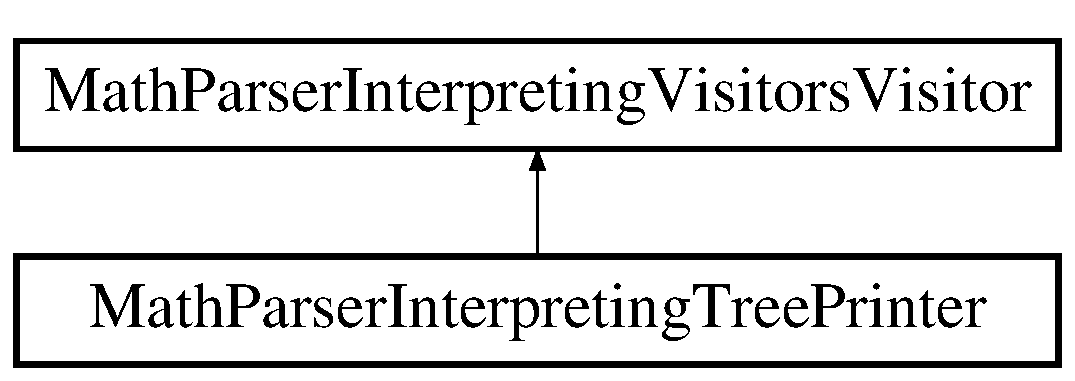
\includegraphics[height=2.000000cm]{classMathParser_1_1Interpreting_1_1TreePrinter}
\end{center}
\end{figure}
\subsection*{Public Member Functions}
\begin{DoxyCompactItemize}
\item 
\hyperlink{classMathParser_1_1Interpreting_1_1TreePrinter_a5d879664f70352a684d925d0225589d3}{visit\-Expression\-Node} (\hyperlink{classMathParser_1_1Parsing_1_1Nodes_1_1ExpressionNode}{Expression\-Node} \$node)
\begin{DoxyCompactList}\small\item\em Interface function for visiting Expression\-Nodes. \end{DoxyCompactList}\item 
\hyperlink{classMathParser_1_1Interpreting_1_1TreePrinter_aff9bf4ad6fc5ea711b23d39b60f0235c}{visit\-Number\-Node} (\hyperlink{classMathParser_1_1Parsing_1_1Nodes_1_1NumberNode}{Number\-Node} \$node)
\begin{DoxyCompactList}\small\item\em Interface function for visiting Number\-Nodes. \end{DoxyCompactList}\item 
\hyperlink{classMathParser_1_1Interpreting_1_1TreePrinter_a9fa160448c7e0a16e907c79c8d3e4f38}{visit\-Variable\-Node} (\hyperlink{classMathParser_1_1Parsing_1_1Nodes_1_1VariableNode}{Variable\-Node} \$node)
\begin{DoxyCompactList}\small\item\em Interface function for visiting Variable\-Nodes. \end{DoxyCompactList}\item 
\hyperlink{classMathParser_1_1Interpreting_1_1TreePrinter_ae5fc098c679ae4e30030bc0a22d621d0}{visit\-Function\-Node} (\hyperlink{classMathParser_1_1Parsing_1_1Nodes_1_1FunctionNode}{Function\-Node} \$node)
\begin{DoxyCompactList}\small\item\em Interface function for visiting Function\-Node. \end{DoxyCompactList}\item 
\hyperlink{classMathParser_1_1Interpreting_1_1TreePrinter_af2b9784abe53d0fa5ddb75528d1a7e8f}{visit\-Constant\-Node} (\hyperlink{classMathParser_1_1Parsing_1_1Nodes_1_1ConstantNode}{Constant\-Node} \$node)
\begin{DoxyCompactList}\small\item\em Interface function for visiting Constant\-Node. \end{DoxyCompactList}\end{DoxyCompactItemize}


\subsection{Detailed Description}
Simple string representation of an A\-S\-T. 

Probably most useful for debugging purposes.

Implementation of a Visitor, transforming an A\-S\-T into a string representation of the tree.

\subsubsection*{Example\-:}


\begin{DoxyCode}
$parser = \textcolor{keyword}{new} StdMathParser();
$f = $parser->parse(\textcolor{stringliteral}{'exp(2x)+xy'});
printer = \textcolor{keyword}{new} TreePrinter();
result = $f->accept($printer);    \textcolor{comment}{// Generates "(+ (exp (* 2 x)) (* x y))"}
\end{DoxyCode}
 

\subsection{Member Function Documentation}
\hypertarget{classMathParser_1_1Interpreting_1_1TreePrinter_af2b9784abe53d0fa5ddb75528d1a7e8f}{\index{Math\-Parser\-::\-Interpreting\-::\-Tree\-Printer@{Math\-Parser\-::\-Interpreting\-::\-Tree\-Printer}!visit\-Constant\-Node@{visit\-Constant\-Node}}
\index{visit\-Constant\-Node@{visit\-Constant\-Node}!MathParser::Interpreting::TreePrinter@{Math\-Parser\-::\-Interpreting\-::\-Tree\-Printer}}
\subsubsection[{visit\-Constant\-Node}]{\setlength{\rightskip}{0pt plus 5cm}Math\-Parser\textbackslash{}\-Interpreting\textbackslash{}\-Tree\-Printer\-::visit\-Constant\-Node (
\begin{DoxyParamCaption}
\item[{{\bf Constant\-Node}}]{\$node}
\end{DoxyParamCaption}
)}}\label{classMathParser_1_1Interpreting_1_1TreePrinter_af2b9784abe53d0fa5ddb75528d1a7e8f}


Interface function for visiting Constant\-Node. 


\begin{DoxyParams}[1]{Parameters}
Constant\-Node & {\em \$node} & Node to visit. \\
\hline
\end{DoxyParams}


Implements \hyperlink{interfaceMathParser_1_1Interpreting_1_1Visitors_1_1Visitor_ac694089225b20c9f848bcfb0a5e600f0}{Math\-Parser\textbackslash{}\-Interpreting\textbackslash{}\-Visitors\textbackslash{}\-Visitor}.

\hypertarget{classMathParser_1_1Interpreting_1_1TreePrinter_a5d879664f70352a684d925d0225589d3}{\index{Math\-Parser\-::\-Interpreting\-::\-Tree\-Printer@{Math\-Parser\-::\-Interpreting\-::\-Tree\-Printer}!visit\-Expression\-Node@{visit\-Expression\-Node}}
\index{visit\-Expression\-Node@{visit\-Expression\-Node}!MathParser::Interpreting::TreePrinter@{Math\-Parser\-::\-Interpreting\-::\-Tree\-Printer}}
\subsubsection[{visit\-Expression\-Node}]{\setlength{\rightskip}{0pt plus 5cm}Math\-Parser\textbackslash{}\-Interpreting\textbackslash{}\-Tree\-Printer\-::visit\-Expression\-Node (
\begin{DoxyParamCaption}
\item[{{\bf Expression\-Node}}]{\$node}
\end{DoxyParamCaption}
)}}\label{classMathParser_1_1Interpreting_1_1TreePrinter_a5d879664f70352a684d925d0225589d3}


Interface function for visiting Expression\-Nodes. 


\begin{DoxyParams}[1]{Parameters}
Expression\-Node & {\em \$node} & Node to visit. \\
\hline
\end{DoxyParams}


Implements \hyperlink{interfaceMathParser_1_1Interpreting_1_1Visitors_1_1Visitor_a201489f6ae0ccc3c25ff153a57994fa1}{Math\-Parser\textbackslash{}\-Interpreting\textbackslash{}\-Visitors\textbackslash{}\-Visitor}.

\hypertarget{classMathParser_1_1Interpreting_1_1TreePrinter_ae5fc098c679ae4e30030bc0a22d621d0}{\index{Math\-Parser\-::\-Interpreting\-::\-Tree\-Printer@{Math\-Parser\-::\-Interpreting\-::\-Tree\-Printer}!visit\-Function\-Node@{visit\-Function\-Node}}
\index{visit\-Function\-Node@{visit\-Function\-Node}!MathParser::Interpreting::TreePrinter@{Math\-Parser\-::\-Interpreting\-::\-Tree\-Printer}}
\subsubsection[{visit\-Function\-Node}]{\setlength{\rightskip}{0pt plus 5cm}Math\-Parser\textbackslash{}\-Interpreting\textbackslash{}\-Tree\-Printer\-::visit\-Function\-Node (
\begin{DoxyParamCaption}
\item[{{\bf Function\-Node}}]{\$node}
\end{DoxyParamCaption}
)}}\label{classMathParser_1_1Interpreting_1_1TreePrinter_ae5fc098c679ae4e30030bc0a22d621d0}


Interface function for visiting Function\-Node. 


\begin{DoxyParams}[1]{Parameters}
Function\-Node & {\em \$node} & Node to visit. \\
\hline
\end{DoxyParams}


Implements \hyperlink{interfaceMathParser_1_1Interpreting_1_1Visitors_1_1Visitor_a497e4a990f99689616c25e76b0ec6ef1}{Math\-Parser\textbackslash{}\-Interpreting\textbackslash{}\-Visitors\textbackslash{}\-Visitor}.

\hypertarget{classMathParser_1_1Interpreting_1_1TreePrinter_aff9bf4ad6fc5ea711b23d39b60f0235c}{\index{Math\-Parser\-::\-Interpreting\-::\-Tree\-Printer@{Math\-Parser\-::\-Interpreting\-::\-Tree\-Printer}!visit\-Number\-Node@{visit\-Number\-Node}}
\index{visit\-Number\-Node@{visit\-Number\-Node}!MathParser::Interpreting::TreePrinter@{Math\-Parser\-::\-Interpreting\-::\-Tree\-Printer}}
\subsubsection[{visit\-Number\-Node}]{\setlength{\rightskip}{0pt plus 5cm}Math\-Parser\textbackslash{}\-Interpreting\textbackslash{}\-Tree\-Printer\-::visit\-Number\-Node (
\begin{DoxyParamCaption}
\item[{{\bf Number\-Node}}]{\$node}
\end{DoxyParamCaption}
)}}\label{classMathParser_1_1Interpreting_1_1TreePrinter_aff9bf4ad6fc5ea711b23d39b60f0235c}


Interface function for visiting Number\-Nodes. 


\begin{DoxyParams}[1]{Parameters}
Number\-Node & {\em \$node} & Node to visit. \\
\hline
\end{DoxyParams}


Implements \hyperlink{interfaceMathParser_1_1Interpreting_1_1Visitors_1_1Visitor_acbcd1cbecf76ba51c893a49746162dc1}{Math\-Parser\textbackslash{}\-Interpreting\textbackslash{}\-Visitors\textbackslash{}\-Visitor}.

\hypertarget{classMathParser_1_1Interpreting_1_1TreePrinter_a9fa160448c7e0a16e907c79c8d3e4f38}{\index{Math\-Parser\-::\-Interpreting\-::\-Tree\-Printer@{Math\-Parser\-::\-Interpreting\-::\-Tree\-Printer}!visit\-Variable\-Node@{visit\-Variable\-Node}}
\index{visit\-Variable\-Node@{visit\-Variable\-Node}!MathParser::Interpreting::TreePrinter@{Math\-Parser\-::\-Interpreting\-::\-Tree\-Printer}}
\subsubsection[{visit\-Variable\-Node}]{\setlength{\rightskip}{0pt plus 5cm}Math\-Parser\textbackslash{}\-Interpreting\textbackslash{}\-Tree\-Printer\-::visit\-Variable\-Node (
\begin{DoxyParamCaption}
\item[{{\bf Variable\-Node}}]{\$node}
\end{DoxyParamCaption}
)}}\label{classMathParser_1_1Interpreting_1_1TreePrinter_a9fa160448c7e0a16e907c79c8d3e4f38}


Interface function for visiting Variable\-Nodes. 


\begin{DoxyParams}[1]{Parameters}
Variable\-Node & {\em \$node} & Node to visit. \\
\hline
\end{DoxyParams}


Implements \hyperlink{interfaceMathParser_1_1Interpreting_1_1Visitors_1_1Visitor_a292630a7204dadd96877d8182f38deb0}{Math\-Parser\textbackslash{}\-Interpreting\textbackslash{}\-Visitors\textbackslash{}\-Visitor}.



The documentation for this class was generated from the following file\-:\begin{DoxyCompactItemize}
\item 
src/\-Math\-Parser/\-Interpreting/Tree\-Printer.\-php\end{DoxyCompactItemize}

\hypertarget{classMathParser_1_1Exceptions_1_1UnknownConstantException}{\section{Math\-Parser\textbackslash{}Exceptions\textbackslash{}Unknown\-Constant\-Exception Class Reference}
\label{classMathParser_1_1Exceptions_1_1UnknownConstantException}\index{Math\-Parser\textbackslash{}\-Exceptions\textbackslash{}\-Unknown\-Constant\-Exception@{Math\-Parser\textbackslash{}\-Exceptions\textbackslash{}\-Unknown\-Constant\-Exception}}
}
Inheritance diagram for Math\-Parser\textbackslash{}Exceptions\textbackslash{}Unknown\-Constant\-Exception\-:\begin{figure}[H]
\begin{center}
\leavevmode
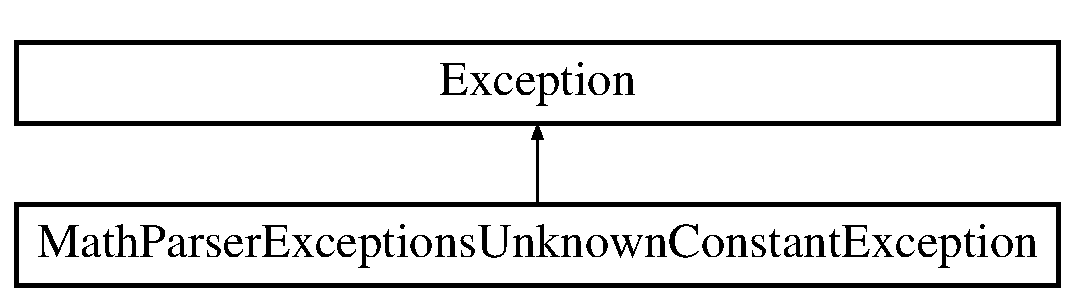
\includegraphics[height=3.000000cm]{classMathParser_1_1Exceptions_1_1UnknownConstantException}
\end{center}
\end{figure}
\subsection*{Public Member Functions}
\begin{DoxyCompactItemize}
\item 
\hypertarget{classMathParser_1_1Exceptions_1_1UnknownConstantException_aaadb7ff0441def32ad66957aa5f3053b}{{\bfseries \-\_\-\-\_\-construct} (\$operator)}\label{classMathParser_1_1Exceptions_1_1UnknownConstantException_aaadb7ff0441def32ad66957aa5f3053b}

\end{DoxyCompactItemize}


The documentation for this class was generated from the following file\-:\begin{DoxyCompactItemize}
\item 
src/\-Math\-Parser/\-Exceptions/Unknown\-Constant\-Exception.\-php\end{DoxyCompactItemize}

\hypertarget{classMathParser_1_1Exceptions_1_1UnknownFunctionException}{\section{Math\-Parser\textbackslash{}Exceptions\textbackslash{}Unknown\-Function\-Exception Class Reference}
\label{classMathParser_1_1Exceptions_1_1UnknownFunctionException}\index{Math\-Parser\textbackslash{}\-Exceptions\textbackslash{}\-Unknown\-Function\-Exception@{Math\-Parser\textbackslash{}\-Exceptions\textbackslash{}\-Unknown\-Function\-Exception}}
}
Inheritance diagram for Math\-Parser\textbackslash{}Exceptions\textbackslash{}Unknown\-Function\-Exception\-:\begin{figure}[H]
\begin{center}
\leavevmode
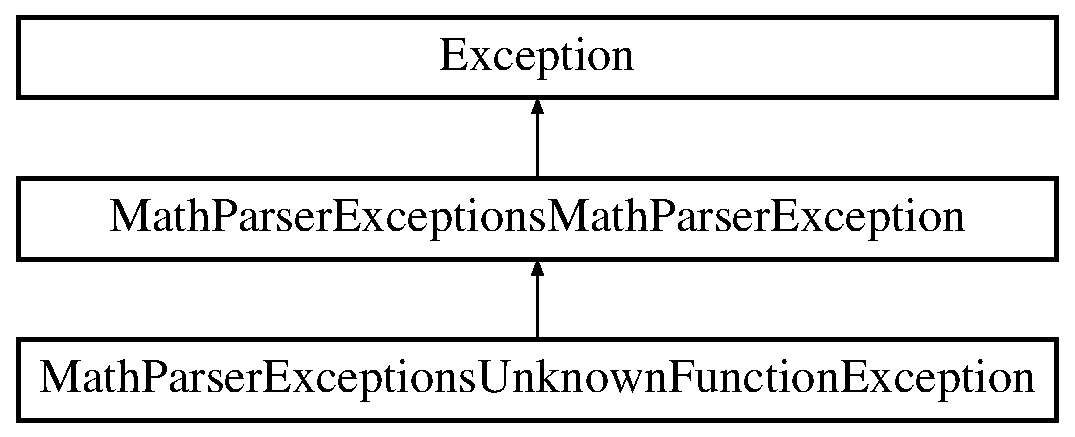
\includegraphics[height=2.000000cm]{classMathParser_1_1Exceptions_1_1UnknownFunctionException}
\end{center}
\end{figure}
\subsection*{Public Member Functions}
\begin{DoxyCompactItemize}
\item 
\hypertarget{classMathParser_1_1Exceptions_1_1UnknownFunctionException_a0bfd13e9eb4aa4b48248917fc5dad3c4}{{\bfseries \-\_\-\-\_\-construct} (\$operator)}\label{classMathParser_1_1Exceptions_1_1UnknownFunctionException_a0bfd13e9eb4aa4b48248917fc5dad3c4}

\end{DoxyCompactItemize}


The documentation for this class was generated from the following file\-:\begin{DoxyCompactItemize}
\item 
src/\-Math\-Parser/\-Exceptions/Unknown\-Function\-Exception.\-php\end{DoxyCompactItemize}

\hypertarget{classMathParser_1_1Exceptions_1_1UnknownNodeException}{\section{Math\-Parser\textbackslash{}Exceptions\textbackslash{}Unknown\-Node\-Exception Class Reference}
\label{classMathParser_1_1Exceptions_1_1UnknownNodeException}\index{Math\-Parser\textbackslash{}\-Exceptions\textbackslash{}\-Unknown\-Node\-Exception@{Math\-Parser\textbackslash{}\-Exceptions\textbackslash{}\-Unknown\-Node\-Exception}}
}
Inheritance diagram for Math\-Parser\textbackslash{}Exceptions\textbackslash{}Unknown\-Node\-Exception\-:\begin{figure}[H]
\begin{center}
\leavevmode
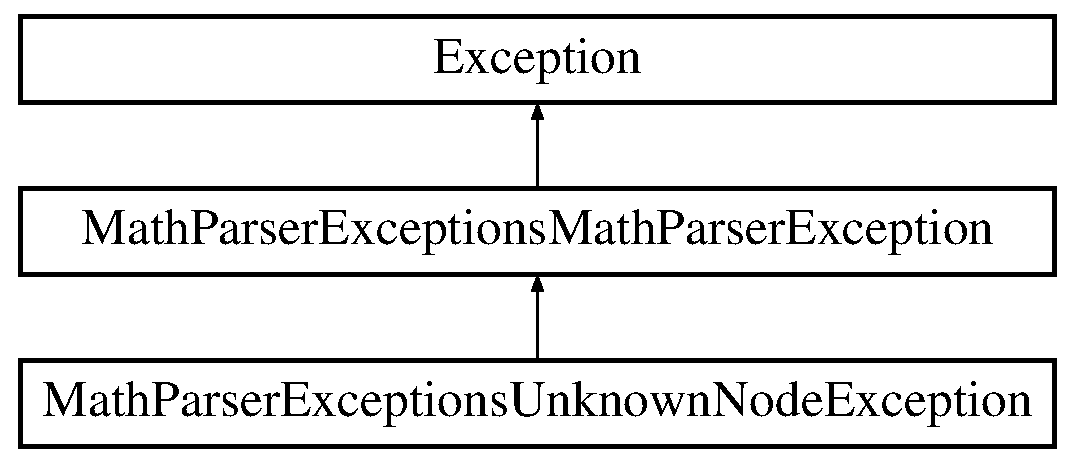
\includegraphics[height=3.000000cm]{classMathParser_1_1Exceptions_1_1UnknownNodeException}
\end{center}
\end{figure}
\subsection*{Public Member Functions}
\begin{DoxyCompactItemize}
\item 
\hypertarget{classMathParser_1_1Exceptions_1_1UnknownNodeException_a05ccf925370ac66946a0a5ebd080aff7}{{\bfseries \-\_\-\-\_\-construct} (\$node)}\label{classMathParser_1_1Exceptions_1_1UnknownNodeException_a05ccf925370ac66946a0a5ebd080aff7}

\end{DoxyCompactItemize}


The documentation for this class was generated from the following file\-:\begin{DoxyCompactItemize}
\item 
src/\-Math\-Parser/\-Exceptions/Unknown\-Node\-Exception.\-php\end{DoxyCompactItemize}

\hypertarget{classMathParser_1_1Exceptions_1_1UnknownOperatorException}{\section{Math\-Parser\textbackslash{}Exceptions\textbackslash{}Unknown\-Operator\-Exception Class Reference}
\label{classMathParser_1_1Exceptions_1_1UnknownOperatorException}\index{Math\-Parser\textbackslash{}\-Exceptions\textbackslash{}\-Unknown\-Operator\-Exception@{Math\-Parser\textbackslash{}\-Exceptions\textbackslash{}\-Unknown\-Operator\-Exception}}
}
Inheritance diagram for Math\-Parser\textbackslash{}Exceptions\textbackslash{}Unknown\-Operator\-Exception\-:\begin{figure}[H]
\begin{center}
\leavevmode
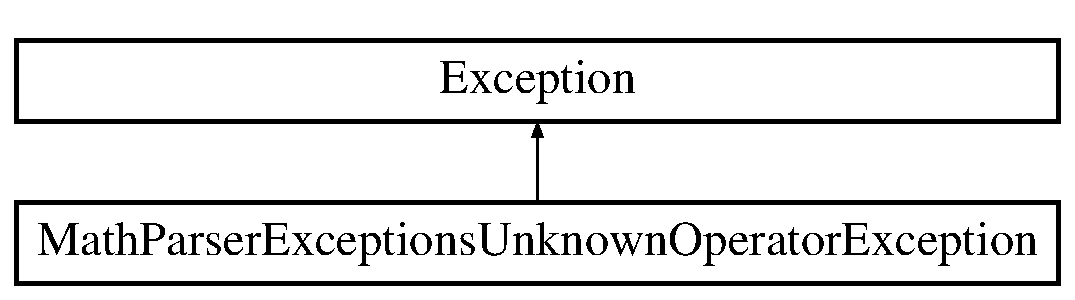
\includegraphics[height=2.000000cm]{classMathParser_1_1Exceptions_1_1UnknownOperatorException}
\end{center}
\end{figure}
\subsection*{Public Member Functions}
\begin{DoxyCompactItemize}
\item 
\hypertarget{classMathParser_1_1Exceptions_1_1UnknownOperatorException_aba135a16c12fbdb536f06b1a16a8c06c}{{\bfseries \-\_\-\-\_\-construct} (\$operator)}\label{classMathParser_1_1Exceptions_1_1UnknownOperatorException_aba135a16c12fbdb536f06b1a16a8c06c}

\end{DoxyCompactItemize}


The documentation for this class was generated from the following file\-:\begin{DoxyCompactItemize}
\item 
src/\-Math\-Parser/\-Exceptions/Unknown\-Operator\-Exception.\-php\end{DoxyCompactItemize}

\hypertarget{classMathParser_1_1Exceptions_1_1UnknownTokenException}{\section{Math\-Parser\textbackslash{}Exceptions\textbackslash{}Unknown\-Token\-Exception Class Reference}
\label{classMathParser_1_1Exceptions_1_1UnknownTokenException}\index{Math\-Parser\textbackslash{}\-Exceptions\textbackslash{}\-Unknown\-Token\-Exception@{Math\-Parser\textbackslash{}\-Exceptions\textbackslash{}\-Unknown\-Token\-Exception}}
}
Inheritance diagram for Math\-Parser\textbackslash{}Exceptions\textbackslash{}Unknown\-Token\-Exception\-:\begin{figure}[H]
\begin{center}
\leavevmode
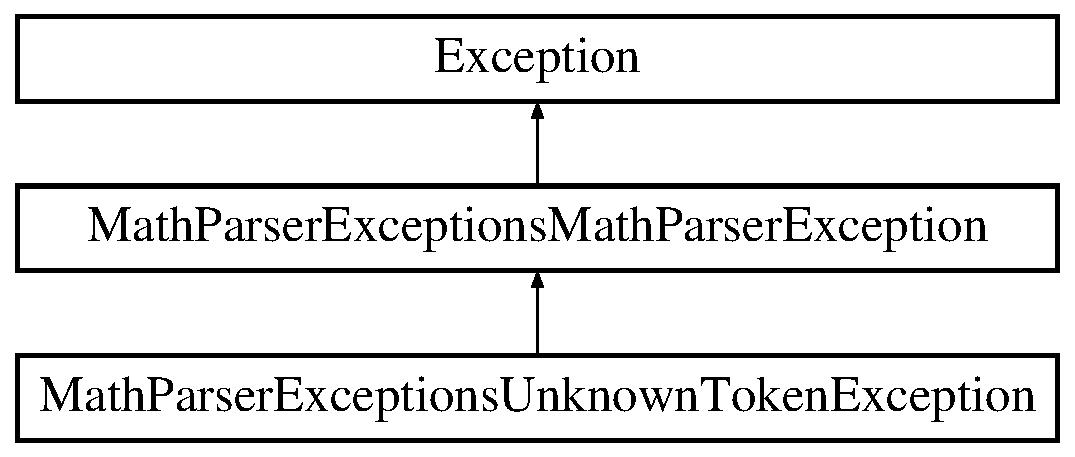
\includegraphics[height=2.000000cm]{classMathParser_1_1Exceptions_1_1UnknownTokenException}
\end{center}
\end{figure}
\subsection*{Public Member Functions}
\begin{DoxyCompactItemize}
\item 
\hypertarget{classMathParser_1_1Exceptions_1_1UnknownTokenException_a7a95d30a218e1bafbe69a9daaa7b34ba}{{\bfseries \-\_\-\-\_\-construct} (\$line, \$column)}\label{classMathParser_1_1Exceptions_1_1UnknownTokenException_a7a95d30a218e1bafbe69a9daaa7b34ba}

\end{DoxyCompactItemize}


The documentation for this class was generated from the following file\-:\begin{DoxyCompactItemize}
\item 
src/\-Math\-Parser/\-Exceptions/Unknown\-Token\-Exception.\-php\end{DoxyCompactItemize}

\hypertarget{classMathParser_1_1Exceptions_1_1UnknownVariableException}{\section{Math\-Parser\textbackslash{}Exceptions\textbackslash{}Unknown\-Variable\-Exception Class Reference}
\label{classMathParser_1_1Exceptions_1_1UnknownVariableException}\index{Math\-Parser\textbackslash{}\-Exceptions\textbackslash{}\-Unknown\-Variable\-Exception@{Math\-Parser\textbackslash{}\-Exceptions\textbackslash{}\-Unknown\-Variable\-Exception}}
}
Inheritance diagram for Math\-Parser\textbackslash{}Exceptions\textbackslash{}Unknown\-Variable\-Exception\-:\begin{figure}[H]
\begin{center}
\leavevmode
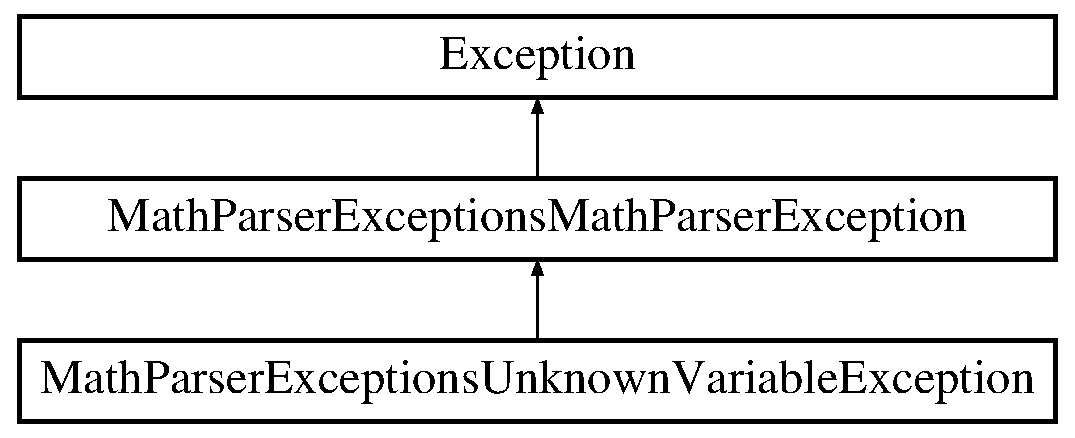
\includegraphics[height=3.000000cm]{classMathParser_1_1Exceptions_1_1UnknownVariableException}
\end{center}
\end{figure}
\subsection*{Public Member Functions}
\begin{DoxyCompactItemize}
\item 
\hypertarget{classMathParser_1_1Exceptions_1_1UnknownVariableException_a040bbcb3b93af9e5a62c4af98b5bc8dd}{{\bfseries \-\_\-\-\_\-construct} (\$variable)}\label{classMathParser_1_1Exceptions_1_1UnknownVariableException_a040bbcb3b93af9e5a62c4af98b5bc8dd}

\end{DoxyCompactItemize}


The documentation for this class was generated from the following file\-:\begin{DoxyCompactItemize}
\item 
src/\-Math\-Parser/\-Exceptions/Unknown\-Variable\-Exception.\-php\end{DoxyCompactItemize}

\hypertarget{classMathParser_1_1Parsing_1_1Nodes_1_1VariableNode}{\section{Math\-Parser\textbackslash{}Parsing\textbackslash{}Nodes\textbackslash{}Variable\-Node Class Reference}
\label{classMathParser_1_1Parsing_1_1Nodes_1_1VariableNode}\index{Math\-Parser\textbackslash{}\-Parsing\textbackslash{}\-Nodes\textbackslash{}\-Variable\-Node@{Math\-Parser\textbackslash{}\-Parsing\textbackslash{}\-Nodes\textbackslash{}\-Variable\-Node}}
}


A\-S\-T node representing a variable.  


Inheritance diagram for Math\-Parser\textbackslash{}Parsing\textbackslash{}Nodes\textbackslash{}Variable\-Node\-:\begin{figure}[H]
\begin{center}
\leavevmode
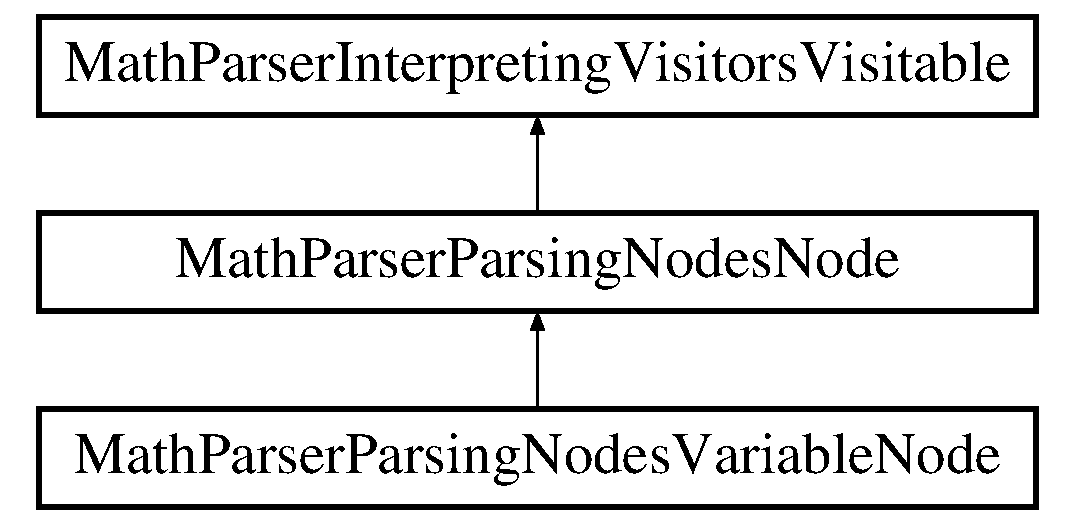
\includegraphics[height=3.000000cm]{classMathParser_1_1Parsing_1_1Nodes_1_1VariableNode}
\end{center}
\end{figure}
\subsection*{Public Member Functions}
\begin{DoxyCompactItemize}
\item 
\hypertarget{classMathParser_1_1Parsing_1_1Nodes_1_1VariableNode_a5a1263313e8f1f7fb82ef1375b0aee77}{{\bfseries \-\_\-\-\_\-construct} (\$name)}\label{classMathParser_1_1Parsing_1_1Nodes_1_1VariableNode_a5a1263313e8f1f7fb82ef1375b0aee77}

\item 
\hyperlink{classMathParser_1_1Parsing_1_1Nodes_1_1VariableNode_abab1fcd4af04ba2981749368d854cfc3}{get\-Name} ()
\begin{DoxyCompactList}\small\item\em Return the name of the variable. \end{DoxyCompactList}\item 
\hypertarget{classMathParser_1_1Parsing_1_1Nodes_1_1VariableNode_a1c41ef12cc6469a2de9c2de325cf6258}{\hyperlink{classMathParser_1_1Parsing_1_1Nodes_1_1VariableNode_a1c41ef12cc6469a2de9c2de325cf6258}{accept} (\hyperlink{interfaceMathParser_1_1Interpreting_1_1Visitors_1_1Visitor}{Visitor} \$visitor)}\label{classMathParser_1_1Parsing_1_1Nodes_1_1VariableNode_a1c41ef12cc6469a2de9c2de325cf6258}

\begin{DoxyCompactList}\small\item\em Implementing the Visitable interface. \end{DoxyCompactList}\end{DoxyCompactItemize}
\subsection*{Private Attributes}
\begin{DoxyCompactItemize}
\item 
\hypertarget{classMathParser_1_1Parsing_1_1Nodes_1_1VariableNode_ac4d263a09ea751c333bb4c30f9e13a0f}{{\bfseries \$name}}\label{classMathParser_1_1Parsing_1_1Nodes_1_1VariableNode_ac4d263a09ea751c333bb4c30f9e13a0f}

\end{DoxyCompactItemize}
\subsection*{Additional Inherited Members}


\subsection{Detailed Description}
A\-S\-T node representing a variable. 

\subsection{Member Function Documentation}
\hypertarget{classMathParser_1_1Parsing_1_1Nodes_1_1VariableNode_abab1fcd4af04ba2981749368d854cfc3}{\index{Math\-Parser\-::\-Parsing\-::\-Nodes\-::\-Variable\-Node@{Math\-Parser\-::\-Parsing\-::\-Nodes\-::\-Variable\-Node}!get\-Name@{get\-Name}}
\index{get\-Name@{get\-Name}!MathParser::Parsing::Nodes::VariableNode@{Math\-Parser\-::\-Parsing\-::\-Nodes\-::\-Variable\-Node}}
\subsubsection[{get\-Name}]{\setlength{\rightskip}{0pt plus 5cm}Math\-Parser\textbackslash{}\-Parsing\textbackslash{}\-Nodes\textbackslash{}\-Variable\-Node\-::get\-Name (
\begin{DoxyParamCaption}
{}
\end{DoxyParamCaption}
)}}\label{classMathParser_1_1Parsing_1_1Nodes_1_1VariableNode_abab1fcd4af04ba2981749368d854cfc3}


Return the name of the variable. 


\begin{DoxyRetVals}{Return values}
{\em string} & \\
\hline
\end{DoxyRetVals}


The documentation for this class was generated from the following file\-:\begin{DoxyCompactItemize}
\item 
src/\-Math\-Parser/\-Parsing/\-Nodes/Variable\-Node.\-php\end{DoxyCompactItemize}

\hypertarget{interfaceMathParser_1_1Interpreting_1_1Visitors_1_1Visitable}{\section{Math\-Parser\textbackslash{}Interpreting\textbackslash{}Visitors\textbackslash{}Visitable Interface Reference}
\label{interfaceMathParser_1_1Interpreting_1_1Visitors_1_1Visitable}\index{Math\-Parser\textbackslash{}\-Interpreting\textbackslash{}\-Visitors\textbackslash{}\-Visitable@{Math\-Parser\textbackslash{}\-Interpreting\textbackslash{}\-Visitors\textbackslash{}\-Visitable}}
}


\hyperlink{interfaceMathParser_1_1Interpreting_1_1Visitors_1_1Visitable}{Visitable} interface,.  


Inheritance diagram for Math\-Parser\textbackslash{}Interpreting\textbackslash{}Visitors\textbackslash{}Visitable\-:\begin{figure}[H]
\begin{center}
\leavevmode
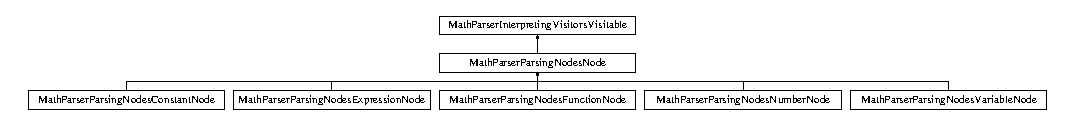
\includegraphics[height=1.249071cm]{interfaceMathParser_1_1Interpreting_1_1Visitors_1_1Visitable}
\end{center}
\end{figure}
\subsection*{Public Member Functions}
\begin{DoxyCompactItemize}
\item 
\hyperlink{interfaceMathParser_1_1Interpreting_1_1Visitors_1_1Visitable_a44418d4bae6a68865102c09dc167409f}{accept} (\hyperlink{interfaceMathParser_1_1Interpreting_1_1Visitors_1_1Visitor}{Visitor} \$visitor)
\begin{DoxyCompactList}\small\item\em Single function in the \hyperlink{interfaceMathParser_1_1Interpreting_1_1Visitors_1_1Visitable}{Visitable} interface. \end{DoxyCompactList}\end{DoxyCompactItemize}


\subsection{Detailed Description}
\hyperlink{interfaceMathParser_1_1Interpreting_1_1Visitors_1_1Visitable}{Visitable} interface,. 

Part of the visitor design pattern implementation. Every Node implements the \hyperlink{interfaceMathParser_1_1Interpreting_1_1Visitors_1_1Visitable}{Visitable} interface, containing the single function \hyperlink{interfaceMathParser_1_1Interpreting_1_1Visitors_1_1Visitable_a44418d4bae6a68865102c09dc167409f}{accept()}

Implemented by the (abstract) Node class.

\paragraph*{Example}


\begin{DoxyCode}
$node = \textcolor{keyword}{new} ExpressionNode(1, \textcolor{charliteral}{'+'}, 2);
$visitor = \textcolor{keyword}{new} TreePrinter();    \textcolor{comment}{// Or any other Visitor}
$node->accept();
\end{DoxyCode}
 

\subsection{Member Function Documentation}
\hypertarget{interfaceMathParser_1_1Interpreting_1_1Visitors_1_1Visitable_a44418d4bae6a68865102c09dc167409f}{\index{Math\-Parser\-::\-Interpreting\-::\-Visitors\-::\-Visitable@{Math\-Parser\-::\-Interpreting\-::\-Visitors\-::\-Visitable}!accept@{accept}}
\index{accept@{accept}!MathParser::Interpreting::Visitors::Visitable@{Math\-Parser\-::\-Interpreting\-::\-Visitors\-::\-Visitable}}
\subsubsection[{accept}]{\setlength{\rightskip}{0pt plus 5cm}Math\-Parser\textbackslash{}\-Interpreting\textbackslash{}\-Visitors\textbackslash{}\-Visitable\-::accept (
\begin{DoxyParamCaption}
\item[{{\bf Visitor}}]{\$visitor}
\end{DoxyParamCaption}
)}}\label{interfaceMathParser_1_1Interpreting_1_1Visitors_1_1Visitable_a44418d4bae6a68865102c09dc167409f}


Single function in the \hyperlink{interfaceMathParser_1_1Interpreting_1_1Visitors_1_1Visitable}{Visitable} interface. 

Calling the \hyperlink{interfaceMathParser_1_1Interpreting_1_1Visitors_1_1Visitable_a44418d4bae6a68865102c09dc167409f}{accept()} function on a \hyperlink{interfaceMathParser_1_1Interpreting_1_1Visitors_1_1Visitable}{Visitable} class, i.\-e. a Node (or subclass thereof) causes the supplied \hyperlink{interfaceMathParser_1_1Interpreting_1_1Visitors_1_1Visitor}{Visitor} to traverse the A\-S\-T.


\begin{DoxyParams}[1]{Parameters}
\hyperlink{interfaceMathParser_1_1Interpreting_1_1Visitors_1_1Visitor}{Visitor} & {\em \$visitor} & \\
\hline
\end{DoxyParams}


Implemented in \hyperlink{classMathParser_1_1Parsing_1_1Nodes_1_1ExpressionNode_a3794b9185ed7928df1f39ec42c557106}{Math\-Parser\textbackslash{}\-Parsing\textbackslash{}\-Nodes\textbackslash{}\-Expression\-Node}, \hyperlink{classMathParser_1_1Parsing_1_1Nodes_1_1FunctionNode_a9796a0fdaf49525adc9ea539b4291835}{Math\-Parser\textbackslash{}\-Parsing\textbackslash{}\-Nodes\textbackslash{}\-Function\-Node}, \hyperlink{classMathParser_1_1Parsing_1_1Nodes_1_1ConstantNode_a5debc023d33ccf262a4c73569b4af841}{Math\-Parser\textbackslash{}\-Parsing\textbackslash{}\-Nodes\textbackslash{}\-Constant\-Node}, \hyperlink{classMathParser_1_1Parsing_1_1Nodes_1_1NumberNode_afe0acdb60d40d8f053a00cddef53a2d4}{Math\-Parser\textbackslash{}\-Parsing\textbackslash{}\-Nodes\textbackslash{}\-Number\-Node}, and \hyperlink{classMathParser_1_1Parsing_1_1Nodes_1_1VariableNode_a1c41ef12cc6469a2de9c2de325cf6258}{Math\-Parser\textbackslash{}\-Parsing\textbackslash{}\-Nodes\textbackslash{}\-Variable\-Node}.



The documentation for this interface was generated from the following file\-:\begin{DoxyCompactItemize}
\item 
src/\-Math\-Parser/\-Interpreting/\-Visitors/Visitable.\-php\end{DoxyCompactItemize}

\hypertarget{interfaceMathParser_1_1Interpreting_1_1Visitors_1_1Visitor}{\section{Math\-Parser\textbackslash{}Interpreting\textbackslash{}Visitors\textbackslash{}Visitor Interface Reference}
\label{interfaceMathParser_1_1Interpreting_1_1Visitors_1_1Visitor}\index{Math\-Parser\textbackslash{}\-Interpreting\textbackslash{}\-Visitors\textbackslash{}\-Visitor@{Math\-Parser\textbackslash{}\-Interpreting\textbackslash{}\-Visitors\textbackslash{}\-Visitor}}
}


\hyperlink{interfaceMathParser_1_1Interpreting_1_1Visitors_1_1Visitor}{Visitor} interface.  


Inheritance diagram for Math\-Parser\textbackslash{}Interpreting\textbackslash{}Visitors\textbackslash{}Visitor\-:\begin{figure}[H]
\begin{center}
\leavevmode
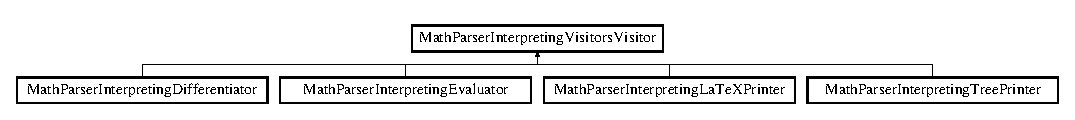
\includegraphics[height=1.166667cm]{interfaceMathParser_1_1Interpreting_1_1Visitors_1_1Visitor}
\end{center}
\end{figure}
\subsection*{Public Member Functions}
\begin{DoxyCompactItemize}
\item 
\hyperlink{interfaceMathParser_1_1Interpreting_1_1Visitors_1_1Visitor_a201489f6ae0ccc3c25ff153a57994fa1}{visit\-Expression\-Node} (\hyperlink{classMathParser_1_1Parsing_1_1Nodes_1_1ExpressionNode}{Expression\-Node} \$node)
\begin{DoxyCompactList}\small\item\em Interface function for visiting Expression\-Nodes. \end{DoxyCompactList}\item 
\hyperlink{interfaceMathParser_1_1Interpreting_1_1Visitors_1_1Visitor_acbcd1cbecf76ba51c893a49746162dc1}{visit\-Number\-Node} (\hyperlink{classMathParser_1_1Parsing_1_1Nodes_1_1NumberNode}{Number\-Node} \$node)
\begin{DoxyCompactList}\small\item\em Interface function for visiting Number\-Nodes. \end{DoxyCompactList}\item 
\hyperlink{interfaceMathParser_1_1Interpreting_1_1Visitors_1_1Visitor_a292630a7204dadd96877d8182f38deb0}{visit\-Variable\-Node} (\hyperlink{classMathParser_1_1Parsing_1_1Nodes_1_1VariableNode}{Variable\-Node} \$node)
\begin{DoxyCompactList}\small\item\em Interface function for visiting Variable\-Nodes. \end{DoxyCompactList}\item 
\hyperlink{interfaceMathParser_1_1Interpreting_1_1Visitors_1_1Visitor_a497e4a990f99689616c25e76b0ec6ef1}{visit\-Function\-Node} (\hyperlink{classMathParser_1_1Parsing_1_1Nodes_1_1FunctionNode}{Function\-Node} \$node)
\begin{DoxyCompactList}\small\item\em Interface function for visiting Function\-Node. \end{DoxyCompactList}\item 
\hyperlink{interfaceMathParser_1_1Interpreting_1_1Visitors_1_1Visitor_ac694089225b20c9f848bcfb0a5e600f0}{visit\-Constant\-Node} (\hyperlink{classMathParser_1_1Parsing_1_1Nodes_1_1ConstantNode}{Constant\-Node} \$node)
\begin{DoxyCompactList}\small\item\em Interface function for visiting Constant\-Node. \end{DoxyCompactList}\end{DoxyCompactItemize}


\subsection{Detailed Description}
\hyperlink{interfaceMathParser_1_1Interpreting_1_1Visitors_1_1Visitor}{Visitor} interface. 

Implemented by every interpreter. The interface specifies functions for visiting and handling each Node subclass. 

\subsection{Member Function Documentation}
\hypertarget{interfaceMathParser_1_1Interpreting_1_1Visitors_1_1Visitor_ac694089225b20c9f848bcfb0a5e600f0}{\index{Math\-Parser\-::\-Interpreting\-::\-Visitors\-::\-Visitor@{Math\-Parser\-::\-Interpreting\-::\-Visitors\-::\-Visitor}!visit\-Constant\-Node@{visit\-Constant\-Node}}
\index{visit\-Constant\-Node@{visit\-Constant\-Node}!MathParser::Interpreting::Visitors::Visitor@{Math\-Parser\-::\-Interpreting\-::\-Visitors\-::\-Visitor}}
\subsubsection[{visit\-Constant\-Node}]{\setlength{\rightskip}{0pt plus 5cm}Math\-Parser\textbackslash{}\-Interpreting\textbackslash{}\-Visitors\textbackslash{}\-Visitor\-::visit\-Constant\-Node (
\begin{DoxyParamCaption}
\item[{{\bf Constant\-Node}}]{\$node}
\end{DoxyParamCaption}
)}}\label{interfaceMathParser_1_1Interpreting_1_1Visitors_1_1Visitor_ac694089225b20c9f848bcfb0a5e600f0}


Interface function for visiting Constant\-Node. 


\begin{DoxyParams}[1]{Parameters}
Constant\-Node & {\em \$node} & Node to visit. \\
\hline
\end{DoxyParams}


Implemented in \hyperlink{classMathParser_1_1Interpreting_1_1Differentiator_ab89f589a9e372a15997cc08608489e1f}{Math\-Parser\textbackslash{}\-Interpreting\textbackslash{}\-Differentiator}, \hyperlink{classMathParser_1_1Interpreting_1_1Evaluator_a257b2634d88050c7e51de91c5f09b7b8}{Math\-Parser\textbackslash{}\-Interpreting\textbackslash{}\-Evaluator}, \hyperlink{classMathParser_1_1Interpreting_1_1LaTeXPrinter_aaa2c3cfcfa01461f52a8f656ef52b92c}{Math\-Parser\textbackslash{}\-Interpreting\textbackslash{}\-La\-Te\-X\-Printer}, and \hyperlink{classMathParser_1_1Interpreting_1_1TreePrinter_af2b9784abe53d0fa5ddb75528d1a7e8f}{Math\-Parser\textbackslash{}\-Interpreting\textbackslash{}\-Tree\-Printer}.

\hypertarget{interfaceMathParser_1_1Interpreting_1_1Visitors_1_1Visitor_a201489f6ae0ccc3c25ff153a57994fa1}{\index{Math\-Parser\-::\-Interpreting\-::\-Visitors\-::\-Visitor@{Math\-Parser\-::\-Interpreting\-::\-Visitors\-::\-Visitor}!visit\-Expression\-Node@{visit\-Expression\-Node}}
\index{visit\-Expression\-Node@{visit\-Expression\-Node}!MathParser::Interpreting::Visitors::Visitor@{Math\-Parser\-::\-Interpreting\-::\-Visitors\-::\-Visitor}}
\subsubsection[{visit\-Expression\-Node}]{\setlength{\rightskip}{0pt plus 5cm}Math\-Parser\textbackslash{}\-Interpreting\textbackslash{}\-Visitors\textbackslash{}\-Visitor\-::visit\-Expression\-Node (
\begin{DoxyParamCaption}
\item[{{\bf Expression\-Node}}]{\$node}
\end{DoxyParamCaption}
)}}\label{interfaceMathParser_1_1Interpreting_1_1Visitors_1_1Visitor_a201489f6ae0ccc3c25ff153a57994fa1}


Interface function for visiting Expression\-Nodes. 


\begin{DoxyParams}[1]{Parameters}
Expression\-Node & {\em \$node} & Node to visit. \\
\hline
\end{DoxyParams}


Implemented in \hyperlink{classMathParser_1_1Interpreting_1_1Differentiator_afed6103538e71009c19d8dd0e37144ee}{Math\-Parser\textbackslash{}\-Interpreting\textbackslash{}\-Differentiator}, \hyperlink{classMathParser_1_1Interpreting_1_1Evaluator_af8dbfe9e89ba2450ca2e070dc39e47e8}{Math\-Parser\textbackslash{}\-Interpreting\textbackslash{}\-Evaluator}, \hyperlink{classMathParser_1_1Interpreting_1_1LaTeXPrinter_a68bcaa8f65dbebd8aadd6002b50dea49}{Math\-Parser\textbackslash{}\-Interpreting\textbackslash{}\-La\-Te\-X\-Printer}, and \hyperlink{classMathParser_1_1Interpreting_1_1TreePrinter_a5d879664f70352a684d925d0225589d3}{Math\-Parser\textbackslash{}\-Interpreting\textbackslash{}\-Tree\-Printer}.

\hypertarget{interfaceMathParser_1_1Interpreting_1_1Visitors_1_1Visitor_a497e4a990f99689616c25e76b0ec6ef1}{\index{Math\-Parser\-::\-Interpreting\-::\-Visitors\-::\-Visitor@{Math\-Parser\-::\-Interpreting\-::\-Visitors\-::\-Visitor}!visit\-Function\-Node@{visit\-Function\-Node}}
\index{visit\-Function\-Node@{visit\-Function\-Node}!MathParser::Interpreting::Visitors::Visitor@{Math\-Parser\-::\-Interpreting\-::\-Visitors\-::\-Visitor}}
\subsubsection[{visit\-Function\-Node}]{\setlength{\rightskip}{0pt plus 5cm}Math\-Parser\textbackslash{}\-Interpreting\textbackslash{}\-Visitors\textbackslash{}\-Visitor\-::visit\-Function\-Node (
\begin{DoxyParamCaption}
\item[{{\bf Function\-Node}}]{\$node}
\end{DoxyParamCaption}
)}}\label{interfaceMathParser_1_1Interpreting_1_1Visitors_1_1Visitor_a497e4a990f99689616c25e76b0ec6ef1}


Interface function for visiting Function\-Node. 


\begin{DoxyParams}[1]{Parameters}
Function\-Node & {\em \$node} & Node to visit. \\
\hline
\end{DoxyParams}


Implemented in \hyperlink{classMathParser_1_1Interpreting_1_1Differentiator_a95027e99c32f63b0689005ff148bee3e}{Math\-Parser\textbackslash{}\-Interpreting\textbackslash{}\-Differentiator}, \hyperlink{classMathParser_1_1Interpreting_1_1Evaluator_a455ab6d3c963aeb2e3ad0c731c8bc081}{Math\-Parser\textbackslash{}\-Interpreting\textbackslash{}\-Evaluator}, \hyperlink{classMathParser_1_1Interpreting_1_1LaTeXPrinter_a85eb667103f7b04abfe3c83e6c0e24a2}{Math\-Parser\textbackslash{}\-Interpreting\textbackslash{}\-La\-Te\-X\-Printer}, and \hyperlink{classMathParser_1_1Interpreting_1_1TreePrinter_ae5fc098c679ae4e30030bc0a22d621d0}{Math\-Parser\textbackslash{}\-Interpreting\textbackslash{}\-Tree\-Printer}.

\hypertarget{interfaceMathParser_1_1Interpreting_1_1Visitors_1_1Visitor_acbcd1cbecf76ba51c893a49746162dc1}{\index{Math\-Parser\-::\-Interpreting\-::\-Visitors\-::\-Visitor@{Math\-Parser\-::\-Interpreting\-::\-Visitors\-::\-Visitor}!visit\-Number\-Node@{visit\-Number\-Node}}
\index{visit\-Number\-Node@{visit\-Number\-Node}!MathParser::Interpreting::Visitors::Visitor@{Math\-Parser\-::\-Interpreting\-::\-Visitors\-::\-Visitor}}
\subsubsection[{visit\-Number\-Node}]{\setlength{\rightskip}{0pt plus 5cm}Math\-Parser\textbackslash{}\-Interpreting\textbackslash{}\-Visitors\textbackslash{}\-Visitor\-::visit\-Number\-Node (
\begin{DoxyParamCaption}
\item[{{\bf Number\-Node}}]{\$node}
\end{DoxyParamCaption}
)}}\label{interfaceMathParser_1_1Interpreting_1_1Visitors_1_1Visitor_acbcd1cbecf76ba51c893a49746162dc1}


Interface function for visiting Number\-Nodes. 


\begin{DoxyParams}[1]{Parameters}
Number\-Node & {\em \$node} & Node to visit. \\
\hline
\end{DoxyParams}


Implemented in \hyperlink{classMathParser_1_1Interpreting_1_1Differentiator_aa6fa0932e84b9f3d778387e48c96a9ef}{Math\-Parser\textbackslash{}\-Interpreting\textbackslash{}\-Differentiator}, \hyperlink{classMathParser_1_1Interpreting_1_1Evaluator_a1ce6d1017e55901a580256a2f1edd027}{Math\-Parser\textbackslash{}\-Interpreting\textbackslash{}\-Evaluator}, \hyperlink{classMathParser_1_1Interpreting_1_1LaTeXPrinter_a5bbb40a11601dc347c9d4ec629723396}{Math\-Parser\textbackslash{}\-Interpreting\textbackslash{}\-La\-Te\-X\-Printer}, and \hyperlink{classMathParser_1_1Interpreting_1_1TreePrinter_aff9bf4ad6fc5ea711b23d39b60f0235c}{Math\-Parser\textbackslash{}\-Interpreting\textbackslash{}\-Tree\-Printer}.

\hypertarget{interfaceMathParser_1_1Interpreting_1_1Visitors_1_1Visitor_a292630a7204dadd96877d8182f38deb0}{\index{Math\-Parser\-::\-Interpreting\-::\-Visitors\-::\-Visitor@{Math\-Parser\-::\-Interpreting\-::\-Visitors\-::\-Visitor}!visit\-Variable\-Node@{visit\-Variable\-Node}}
\index{visit\-Variable\-Node@{visit\-Variable\-Node}!MathParser::Interpreting::Visitors::Visitor@{Math\-Parser\-::\-Interpreting\-::\-Visitors\-::\-Visitor}}
\subsubsection[{visit\-Variable\-Node}]{\setlength{\rightskip}{0pt plus 5cm}Math\-Parser\textbackslash{}\-Interpreting\textbackslash{}\-Visitors\textbackslash{}\-Visitor\-::visit\-Variable\-Node (
\begin{DoxyParamCaption}
\item[{{\bf Variable\-Node}}]{\$node}
\end{DoxyParamCaption}
)}}\label{interfaceMathParser_1_1Interpreting_1_1Visitors_1_1Visitor_a292630a7204dadd96877d8182f38deb0}


Interface function for visiting Variable\-Nodes. 


\begin{DoxyParams}[1]{Parameters}
Variable\-Node & {\em \$node} & Node to visit. \\
\hline
\end{DoxyParams}


Implemented in \hyperlink{classMathParser_1_1Interpreting_1_1Differentiator_a52cc092817e78043da5e6bd86e09ff9f}{Math\-Parser\textbackslash{}\-Interpreting\textbackslash{}\-Differentiator}, \hyperlink{classMathParser_1_1Interpreting_1_1Evaluator_a67cd18f0dc33f6e2755008053cd8cc0a}{Math\-Parser\textbackslash{}\-Interpreting\textbackslash{}\-Evaluator}, \hyperlink{classMathParser_1_1Interpreting_1_1LaTeXPrinter_aced38823c7de0b9ad84884028370a8d2}{Math\-Parser\textbackslash{}\-Interpreting\textbackslash{}\-La\-Te\-X\-Printer}, and \hyperlink{classMathParser_1_1Interpreting_1_1TreePrinter_a9fa160448c7e0a16e907c79c8d3e4f38}{Math\-Parser\textbackslash{}\-Interpreting\textbackslash{}\-Tree\-Printer}.



The documentation for this interface was generated from the following file\-:\begin{DoxyCompactItemize}
\item 
src/\-Math\-Parser/\-Interpreting/\-Visitors/Visitor.\-php\end{DoxyCompactItemize}

%--- End generated contents ---

% Index
\newpage
\phantomsection
\addcontentsline{toc}{chapter}{Index}
\printindex

\end{document}
